%!TEX TS-program = xelatex
\documentclass[10pt,twoside,table]{article}\usepackage[]{graphicx}\usepackage[]{color}

\usepackage{alltt}
\usepackage{graphicx}
\usepackage{gensymb}
\usepackage[top=1cm, bottom=1.5cm, left=1.2cm, right=1.2cm]{geometry}
\usepackage[font=small]{caption}
\usepackage{adjustbox}
\usepackage{fancyhdr}
\usepackage{layout}
\usepackage{booktabs}
\usepackage{kpfonts}
\usepackage[explicit]{titlesec}
\usepackage{wrapfig}
\usepackage{tcolorbox}
\usepackage{xcolor}
\usepackage{setspace}
\usepackage{parskip}
\usepackage{tikz}
\usepackage{fontspec}
\usepackage{anyfontsize}
\usepackage{hyperref}

%\usepackage[table]{xcolor}

\setmainfont{Calibri}

% Headers and Footers
\pagestyle{fancy}
\renewcommand{\headrulewidth}{0pt}
\rhead{}
\lhead{}
\cfoot{}
\fancyfoot[LE,RO]{\thepage}

% Box line thickness setting
\setlength{\fboxrule}{1.5pt}

\setlength{\headsep}{0.2in}

\newcommand*{\ChapterFont}{%
	\fontseries{b}
	\doublespacing
	\fontsize{40}{20}%
	\color{white}
	\pagecolor{2dblue}
	\selectfont}

\newcommand*{\PageHeading}[1]{%
	\begin{tikzpicture}[remember picture,overlay]
		\node[anchor=north west,minimum width=21.6cm,minimum height=2cm,fill=2dblue, font=\bf,align=center,text=white] (RB) at (current page.north west){\Large #1};
	\end{tikzpicture}}


\newcommand*{\SectionHeading}[2]{%
	\begin{tikzpicture}[remember picture,overlay]
	\node[anchor=south west, yshift = 4cm ,minimum width=21.6cm,minimum height=6cm,fill=2dblue, text width=18cm, font=\bf,text=white] (RB) at (current page.south west){\Huge #1};
	\node[anchor=south west, yshift = 2.9cm ,minimum width=21.6cm,minimum height=6cm, text width=18cm, font=\bf,text=white] (RB) at (current page.south west){\Huge #2};
	\end{tikzpicture}}





\setlength{\parskip}{1em}

%Sets size and colour: section titles
\renewcommand{\familydefault}{\sfdefault}
\usepackage{xcolor}
\definecolor{2dblue}{RGB}{8, 70, 101}
\definecolor{backgroundgrey}{RGB}{242,242,242}
%\definecolor{redbox}{RGB}{192,0,0}
%\definecolor{bluebox}{RGB}{33,89,104}
\usepackage{titlesec}
\titleformat{\section}
{\normalfont\Large\centering\bfseries\color{2dblue}}
{\thesection}{1em}{}


% Box with a shaded border
\newtcolorbox{shadedbox}{
%	drop shadow southeast,
%	breakable,
%	enhanced jigsaw,
	colback=white,
}

% Sets table border width
\setlength{\arrayrulewidth}{.8mm}
\definecolor{lightgrey}{rgb}{0.95,0.95,0.95}

\IfFileExists{upquote.sty}{\usepackage{upquote}}{}



\begin{document}
	\section*{P1} % Front Cover
		\thispagestyle{empty}
		\pagecolor{2dblue}
		\begin{center}
			
		{\Huge\color{white}{
			\textbf{
				California Insurances Climate Alignment Tests
			}
			\par
			2018}}
		\vspace{2cm}
	
		{\fontsize{26pt}{30pt}\selectfont\color{white}\textbf{ReportInsuranceName}\par}
	
		\vspace{1cm}
	
		\adjincludegraphics[height=14cm,trim={0cm 0cm 0cm 0cm},clip]{ReportGraphics/Picture1}	
			
		\end{center}
	
	\begin{tikzpicture}[remember picture,overlay]
	\node[anchor=south west, yshift = 0cm ,minimum width=21.6cm,minimum height=4cm,fill=white] (RB) at (current page.south west){
		\adjincludegraphics[height=2.8cm,trim={0cm 0cm 0cm 0cm},clip]{ReportGraphics/Logo_front}
		\hspace{3.5cm}
		\adjincludegraphics[height=2.8cm,trim={0cm 0cm 0cm 0cm},clip]{ReportGraphics/PACTA_Logo}};
	\end{tikzpicture}
	
	\newpage
	\pagecolor{white}
	\section*{P2} % Exec Summary p1
	\PageHeading{EXECUTIVE SUMMARY}
	
	\setlength\intextsep{0pt}	
	\begin{wrapfigure}{r}{0.49\linewidth}
		
		
		\begin{center}
			{\rowcolors{2}{white}{lightgrey}
				\setlength{\tabcolsep}{10pt} % Default value: 6pt
				\renewcommand{\arraystretch}{1.5} % Default value: 1
				\begin{tabular}{ p{.35\linewidth} p{.49\linewidth} }
					\hline
					\multicolumn{2}{c}{\textbf{Scope of Analysis}} \\
					\hline
					Insurance Name & ReportInsuranceName  \\ 
					Size of portfolio (in \$) & SizeofPortfolio  \\ 
					Scenario & IEA 2° Scenario  \\ 
					Geography - \newline Financial Assets & Global \\ 
					Geography - \newline Economic Assets & Global  \\ 
					Asset Class & Listed Equity, Corporate Bonds \\ 
					Portfolio Timestamp & 12.31.2016  \\ 
					Peers & NoPeers California Insurance Companies  \\
					\hline
				\end{tabular}
			}
			
		\end{center}

		\vspace{.2cm}
				
		\textbf{Est. share of the portfolio exposed to business activities covered in the International Energy Agency 2°C scenario}
		
		\centering{\adjincludegraphics[width = .8\linewidth,trim={0cm 0.2cm 0cm .4cm},clip]{CAFigures/Fig01}	}
		
		\vspace{-5.5cm}
		
	\end{wrapfigure}
	\textbf{This report provides a 2°C scenario analysis on your financial portfolio.} 
	
	It responds to the recommendations of the Financial Stability Board Task Force on Climate-Related Financial Disclosures. Over 1,000 financial institutions have been assessed using the model applied in this report, as part of direct partnerships with over 200 institutional investors, and collaborations with  a number of financial supervisory authorities. 
	
	The outputs provided in this report – based on the scope of analysis summarized in the table on the right – provide an analysis of the portfolio relative to an economic transition consistent with limiting global warming to 2°C above pre-industrial levels, as well as a comparision to peers. The analysis provides answers to three questions: 
	
	\begin{enumerate}
		\item{What is my exposure to the 2°C scenario today?}
		\item{Is my portfolio building or reducing risk in terms of being aligned / misaligned with a 2°C transition over the next 5 years?}
		\item{What is my expected transition risk exposure?}
	\end{enumerate}
	
	\textbf{The figure on the right and below shows the \% of the portfolio exposed to the energy, power, transport, and other high-carbon sectors.}
	
	The figure below in turn shows the breakdown within these exposures, notably power, fossil fuels, and automotive, to different technologies and fuels.
		
	\vspace{2.2cm}
	
	\centerline{
		\begin{minipage}[t]{.3\linewidth}
			\begin{tcolorbox}[text width=.8\linewidth]
				\textbf{FFSectorPortEQ \%} of your portfolio is invested in the Fossil Fuel sector \newline
				\textbf{FFSectorPeerEQ \%} is the peer group average.
			\end{tcolorbox}
		\end{minipage}
		\hspace{.02\linewidth}
		\begin{minipage}[t]{.3\linewidth}
			\begin{tcolorbox}[text width=.8\linewidth]
				\textbf{PowerSectorPortEQ \%} of your portfolio is invested in the Power sector \newline
				\textbf{PowerSectorPeerEQ \%} is the peer group average.
			\end{tcolorbox}
		\end{minipage}
		\hspace{.02\linewidth}
		\begin{minipage}[t]{.3\linewidth}
			\begin{tcolorbox}[text width=.8\linewidth]
				\textbf{AutoSectorPortEQ \%} of your portfolio is invested in the Automotive sector \newline
				\textbf{AutoSectorPeerEQ \%} is the peer group average.
			\end{tcolorbox}
		\end{minipage}
	}
	
	\vspace{-0.5cm}
	\adjincludegraphics[width = 1\linewidth,trim={0cm 1cm 0cm 0cm},clip]{CAFigures/Fig02}	
	
	\newpage
	




	\newpage
%\end{document}
	\section*{P3} % Exec Summary p2
	\PageHeading{EXECUTIVE SUMMARY}
	
	\textbf{The figure below shows the extent to which the production / investment trend in the portfolio is consistent with the trend in the 2°C scenario.}
		
		It compares the portfolio trend to a 2°C trendline that is normalized to a growth / decline of 1 over the next 5 years for each technology. The chart on the left shows the evolution for low-carbon technologies and on the right for high-carbon technologies – aggregated across all of the portfolios analysed in the report. 
		
		The results can be interpreted based on assessing whether the portfolios are aligned with the 2°C scenario trend as defined by the International Energy Agency. They also potentially highlight whether the portfolio is building or reducing risk in terms of investing in assets today that are misaligned with a 2°C pathway or failing to invest in assets that will drive the transition.
				
	
		\begin{minipage}[t]{.49\linewidth}
		\textbf{THE TREND FOR THE PORTFOLIO FOR LOW-CARBON TECHNOLOGIES RELATIVE TO THE 2°C SCENARIO
		 }
		
		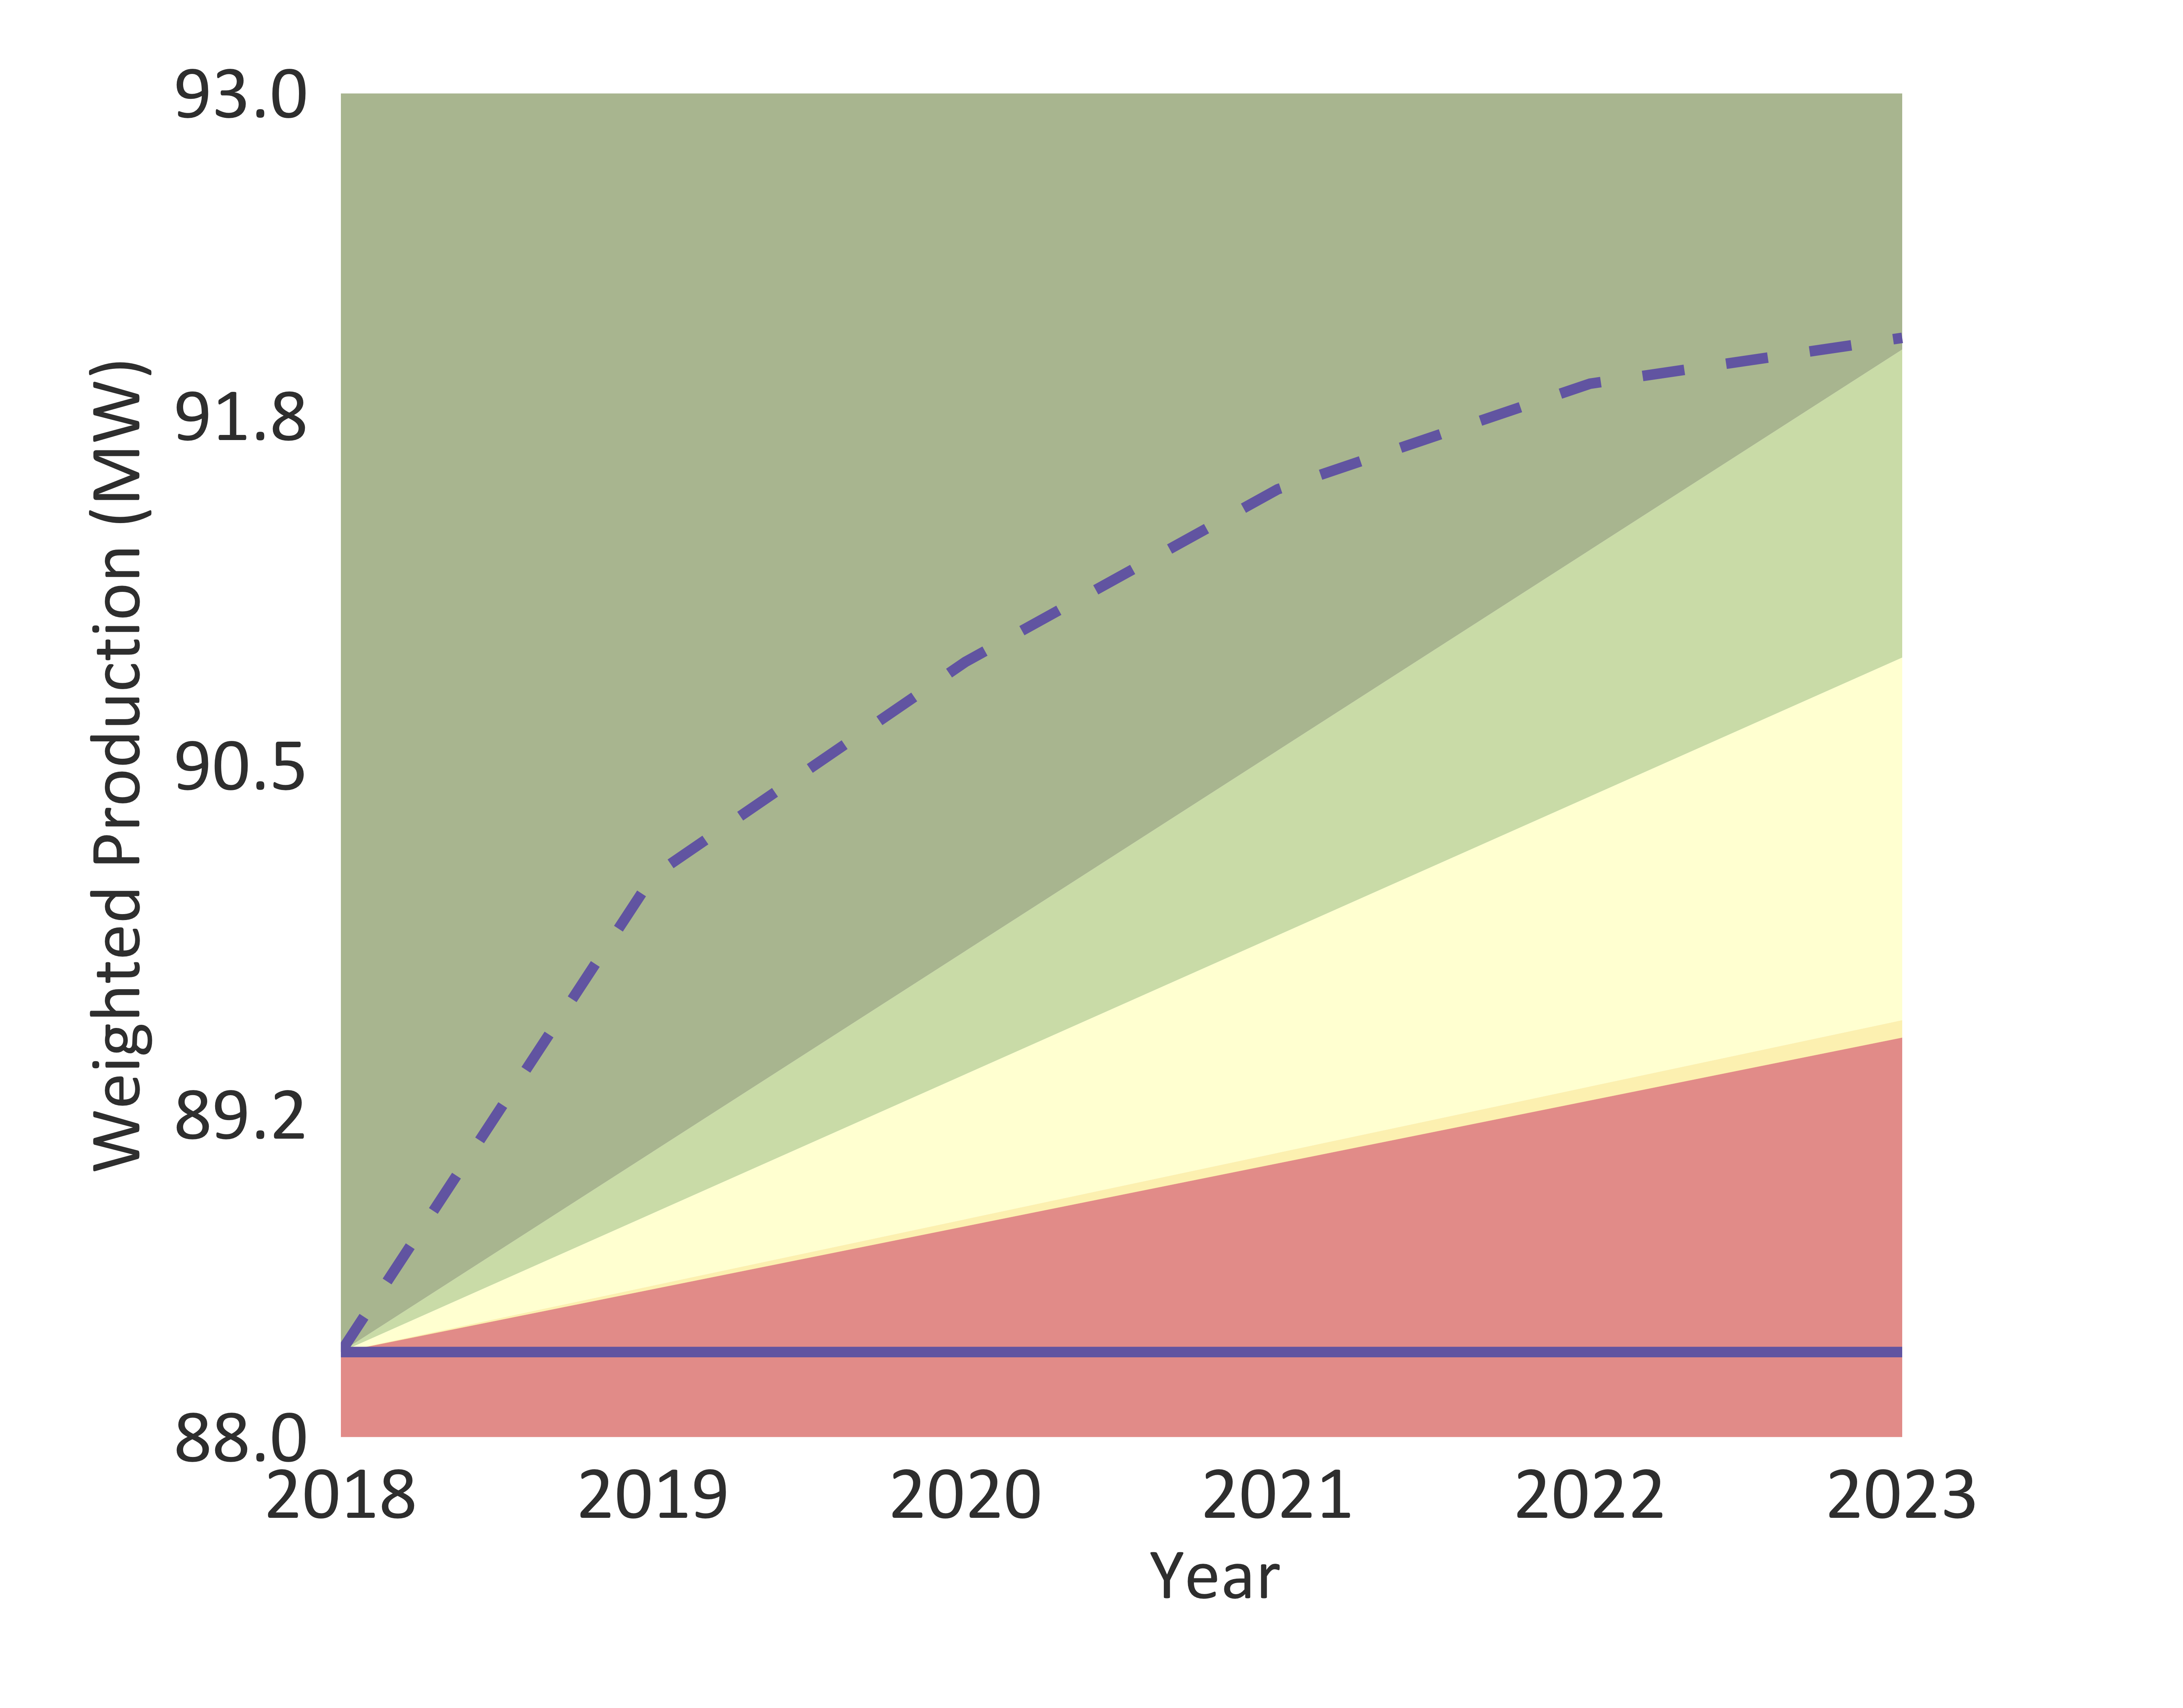
\includegraphics[trim = {0 0cm 0 0},width=1\linewidth]{CAFigures/Fig10}
		
	\end{minipage}	
	\hspace{.02\linewidth}
	\begin{minipage}[t]{.49\textwidth}
		\textbf{THE TREND FOR THE PORTFOLIO FOR HIGH-CARBON TECHNOLOGIES RELATIVE TO THE 2°C SCENARIO
		 }
		
		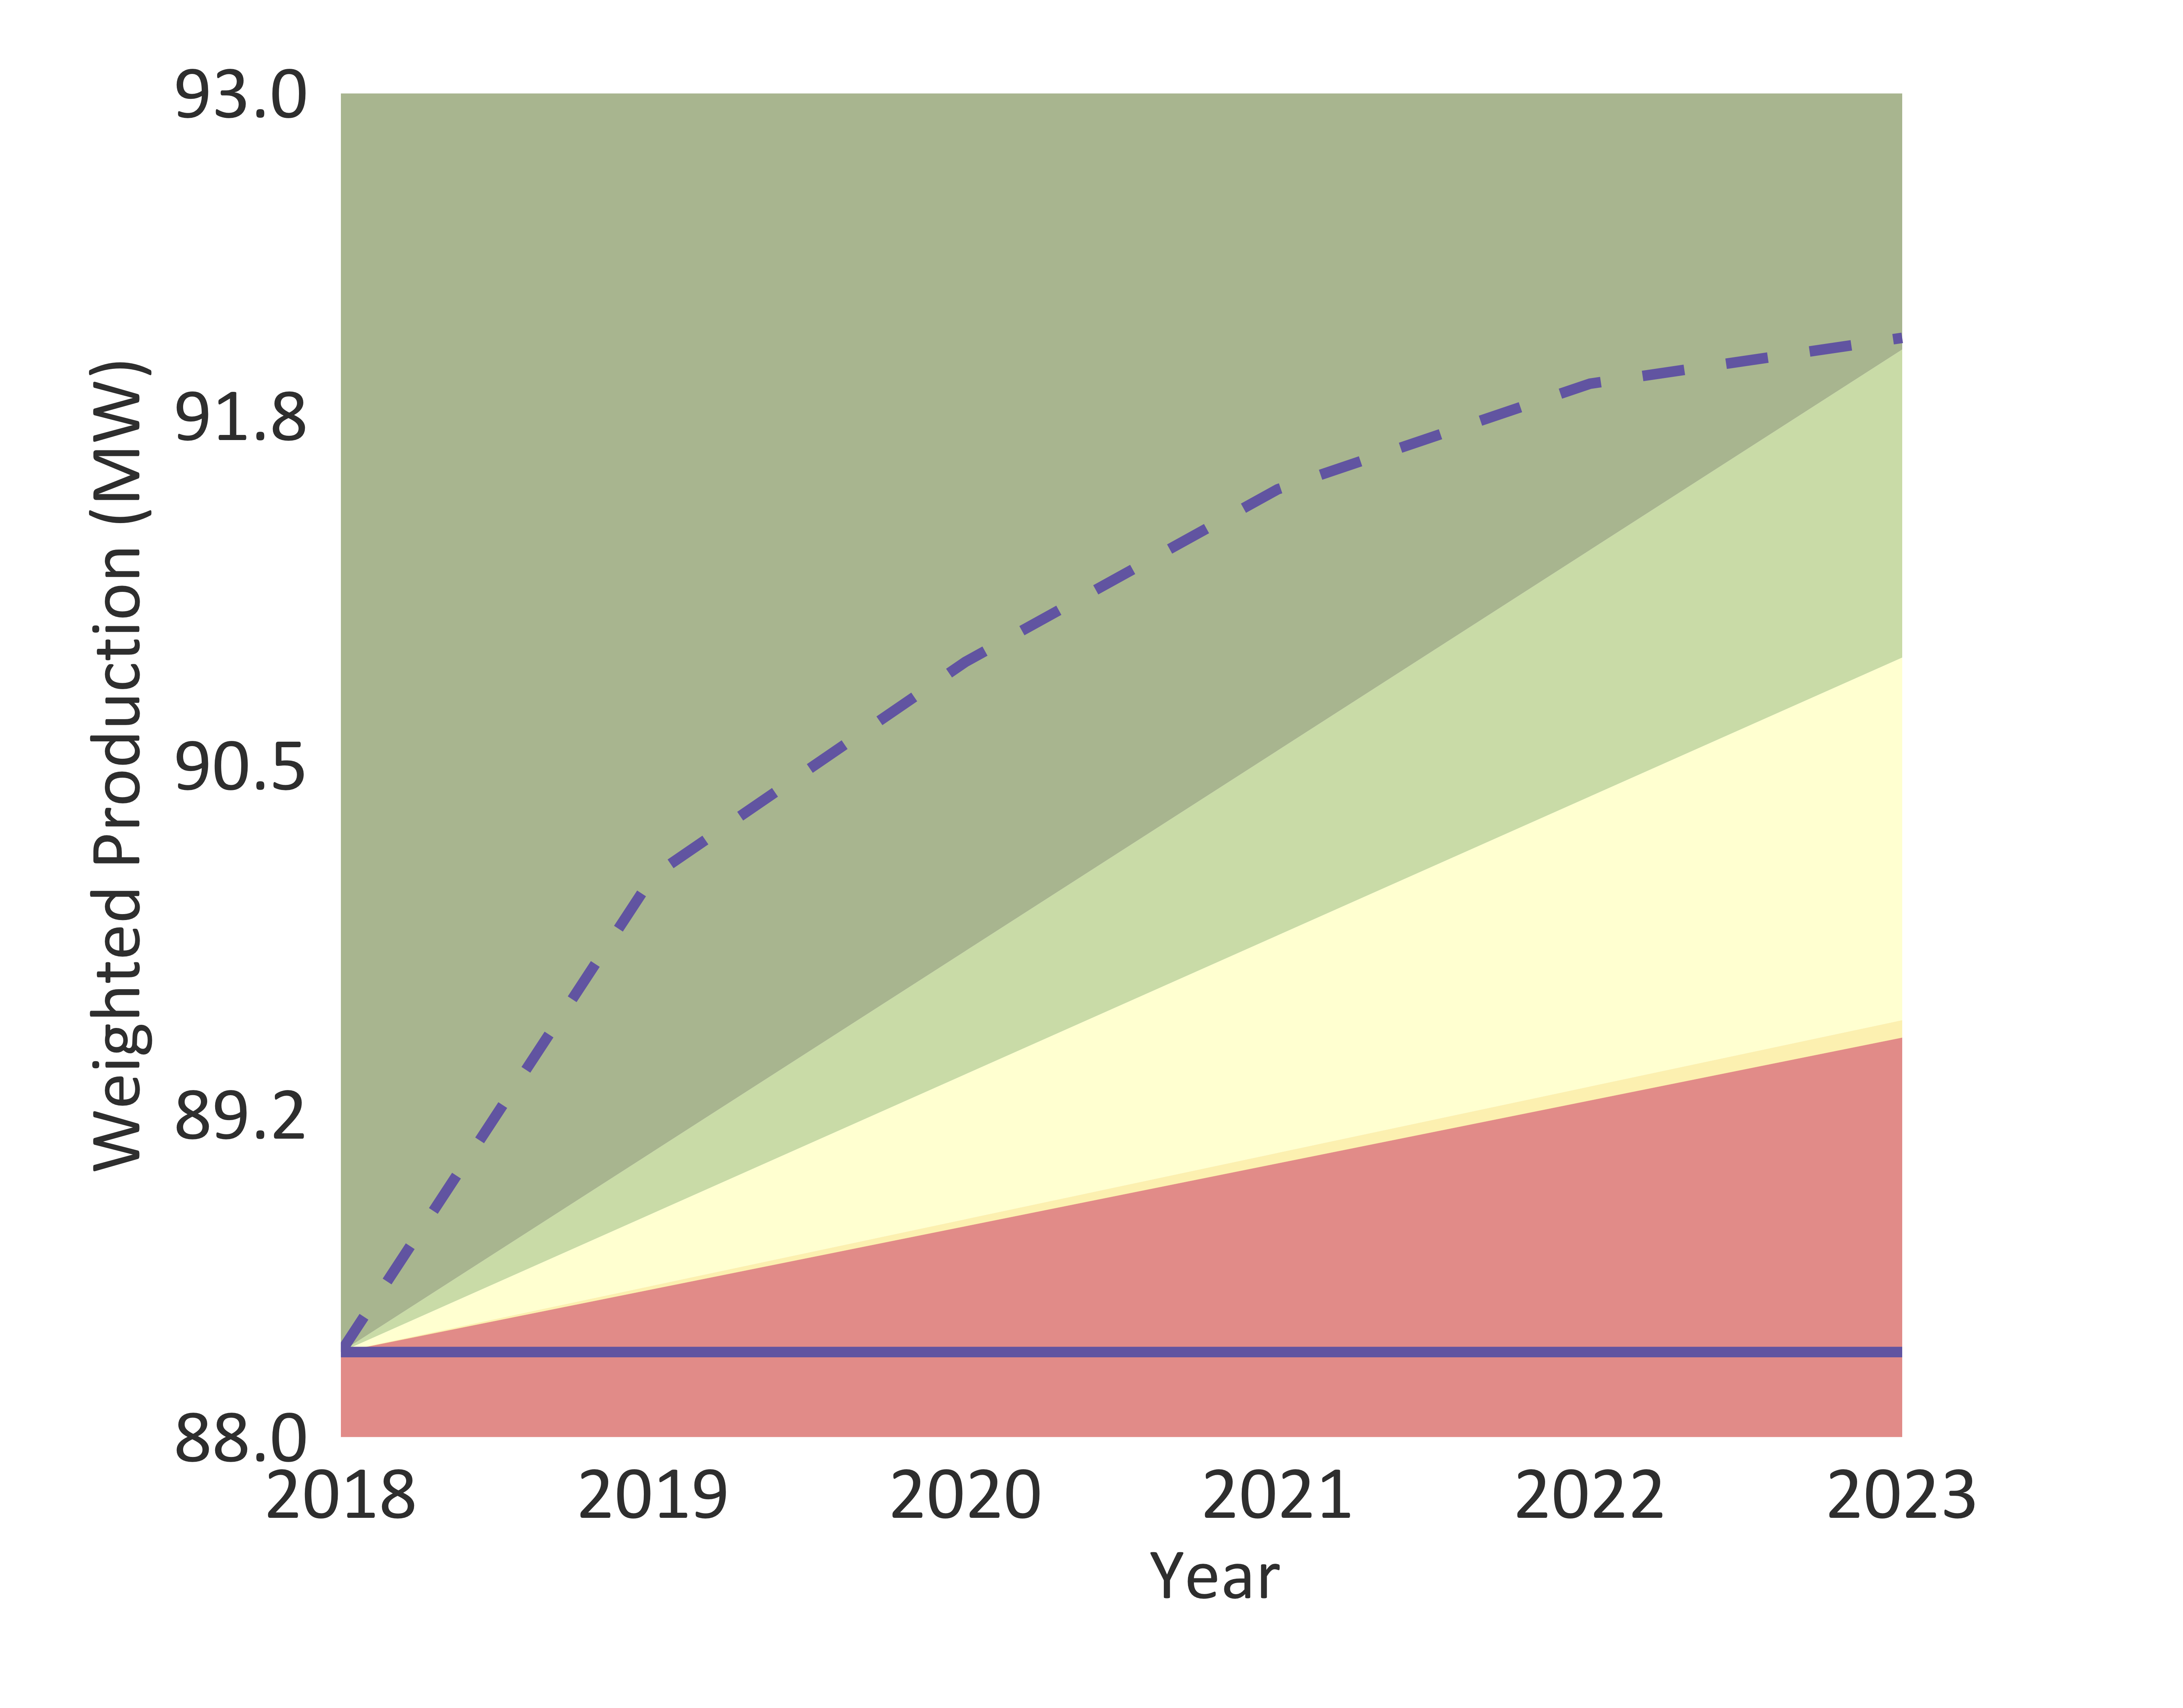
\includegraphics[trim = {0 0cm 0 0},width=1\linewidth]{CAFigures/Fig10}
				

	\end{minipage}
	
	\textbf{The figure below shows a broader ‘transition risk’ exposure for the corporate bonds portfolio, based on a sector classification system developed by Moody’s.}
	
	The results show the percent of your corporate bonds portfolios exposed to ‘environmental risks’ as defined by Moody’s compared to your peers analysed in the context of this assessment. The analysis is based on a top-down sector classification system and thus does not distinguish low-carbon from high-carbon exposures within a sector.
	
		
	\textbf{THE ENVIRONMENTAL RISK EXPOSURE OF YOUR PORTFOLIO RELATIVE TO ITS PEERS}	
	
	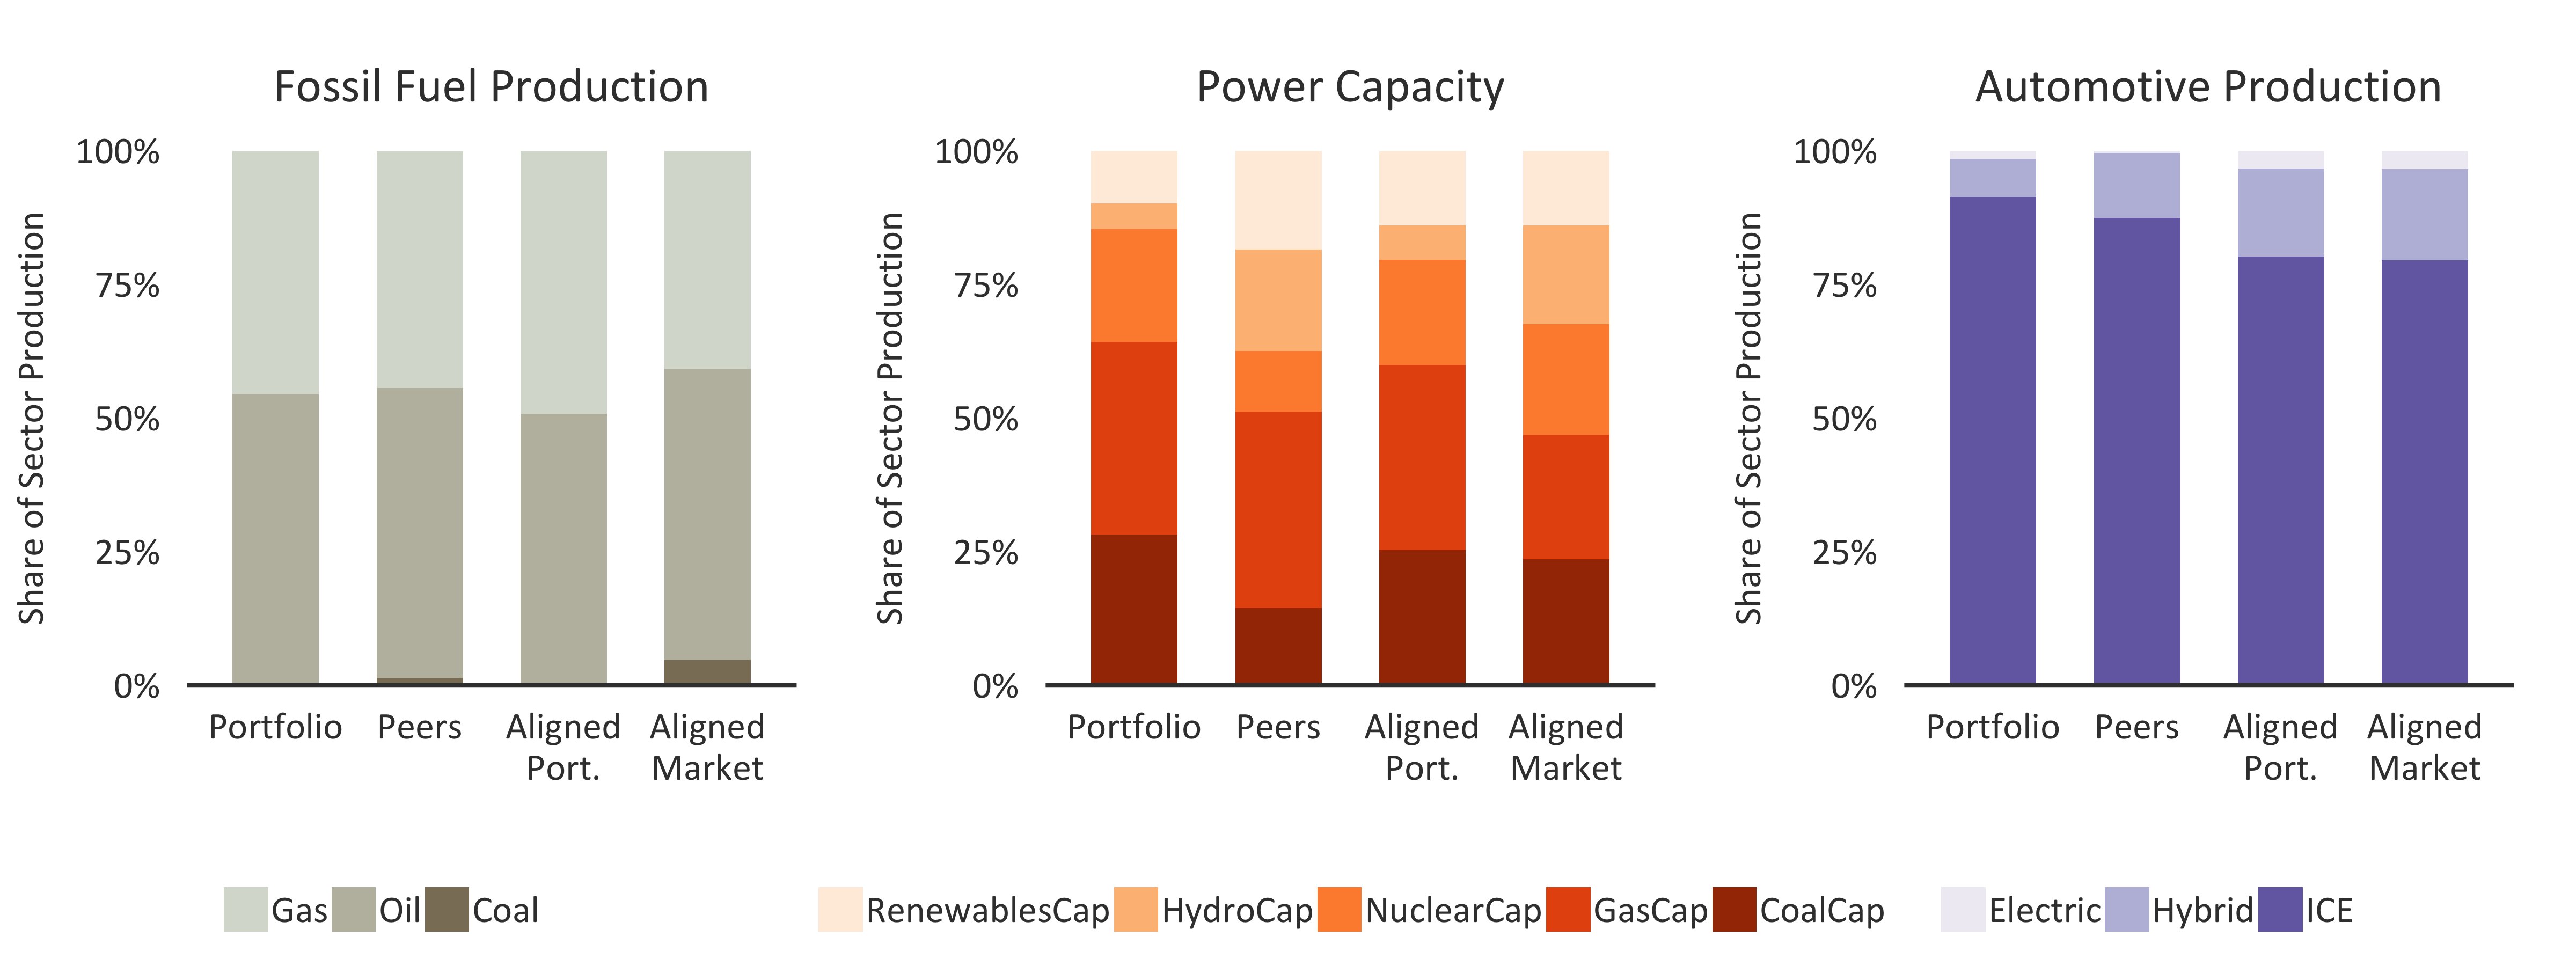
\includegraphics[trim = {0 0cm 0 0},width=1\linewidth]{CAFigures/Fig05}		
			
			
	\newpage
	\section*{P4} % 1st Section
	\thispagestyle{empty}
	\vspace{17cm}
	\SectionHeading{Section 1:}{Introduction}
	
	\newpage
	\singlespacing
	\normalfont
	\pagecolor{white}
	\color{black}
	
	\newpage
	\section*{P5} % Report Contents
	\PageHeading{REPORT CONTENTS}
	
	\textbf{This report provides a 2°C scenario analysis of your equity and corporate bond portfolios, following the recommendations of the Financial Stability Board Task Force on Climate-Related Financial Disclosures (FSB TCFD). Specifically, it seeks to inform the reader about three issues.}
	
	\begin{enumerate}
		\item{\textbf{What is my exposure to the 2°C scenario and transition risk today? (Section 2)}
		}
		
		The first part of the report summarizes the exposures of the portfolio (in terms of \% of the portfolio) to business activities potentially affected by the transition to a low-carbon economy and by extension more broadly its exposure to transition risk. Specifically, it will quantify the percent of the portfolio that can be included in 2°C scenario analysis, the relative exposure to low-carbon and high-carbon fuels and technologies across the energy, power, and automobile sector, as well as the application of the Moody’s environmental risk assessment framework on the corporate bonds portfolio. The analysis will also benchmark the results to the peers included in this framework.
	
		\item{\textbf{Is my portfolio building or reducing risk in terms of being aligned / misaligned with a 2°C transition over the next 5 years? (Section 3)}
		}
		
		The second part of the report will quantify the extent to which the portfolio is building or reducing risk in terms of being aligned / misaligned with the 2°C scenario pathway over the next 5 years across key business activities. The analysis will focus on the fossil fuel related sectors in terms of energy (oil production, gas production), electric power (renewables, coal power), and automobile (Internal combustion engine vehicles – gas, diesel – and electric vehicles). The analysis will show the forward-looking production / investment trend in the portfolio and compare that to the regionally-weighted trend of the scenario. The results will be compared to the global stock and bond market averages, as well as the peer-average for California insurance companies.
	
		\item{\textbf{What is my expected exposure in 5 five years? (Section 4)}
		}
		
		The third part of the report will quantify the extent to which the portfolio over- or under-weights high-carbon and low-carbon technologies / fuels in five years, relative to the stock and bond market if it is on a 2°C transition and the actual stock and bond market.
		
		\item{\textbf{What is driving the results? (Section 5)}}
		
		The final section will provide some more granular information on the companies behind the securities in your portfolio and the extent to which they are driving the results.
		
		You will also be able to find further background information on the scenarios nad modelling at the end of the report.
		
	
	\end{enumerate}

	\vspace{1cm}

	\begin{shadedbox}
		\textbf{Section 1: }Introduction
		
		\textbf{Section 2: }Exposure 2018 to transition risk and 2°C scenario
		
		\textbf{Section 3: }Evolution of the transition risk and alignment with 2°C scenarios
		
		\textbf{Section 4: }Exposure 2023
		
		\textbf{Section 5: }Company information
		
		\textbf{Section 6: }Capacity building on 2° transition scenarios and methodology
		
	\end{shadedbox}

	\newpage
	\section*{P6} % 2nd Section
	\thispagestyle{empty}
	\vspace{17cm}
	\SectionHeading{Section 2:}{THE CURRENT EXPOSURE}
	
	\newpage
	\singlespacing
	\normalfont
	\pagecolor{white}
	\color{black}
	
	\newpage	
	\section*{P7} % 2° Scenario - Current Exposure 2018
	\PageHeading{2° SCENARIO - CURRENT EXPOSURE 2018}	
	
	\setlength\intextsep{0pt}
	\begin{wrapfigure}{r}{0.5\linewidth}
		\vspace{-.3cm}
		\textbf{Est. share of the portfolio exposed to business activities covered in the International Energy Agency 2°C scenario}
		
		\vspace{-.2cm}
		\center{\adjincludegraphics[width = .8\linewidth,trim={0cm 0.2cm 0cm 0cm},clip]{CAFigures/Fig01}	}
		\vspace{-2.2cm}
		\newline
		
	\end{wrapfigure}
	
	\textbf{This page provides information on the exposure of the portfolios to business activities in 2°C scenarios. }
	
	These business activities identified below account for roughly 70-90\% of GHG emissions in the typical investor portfolio. The figure on the right shows the percent of the portfolio (by asset class) exposed to the energy, power, transport, and other high-carbon sectors. The figures below in turn show for the portfolio (by asset class) the weight of each fuel / technology for fossil fuel production, power capacity, and automobile production. It highlights the extent to which the portfolio – within its 2°C scenario exposure – is exposed to a higher or lower degree to different types of high-carbon and low-carbon fuels and technologies.
	
	
	This is more text that addesses the sector selection.This is more text that addesses the sector selection.This is more text that addesses the sector selection.This is more text that addesses the sector selection.This is more text that addesses.
	
	\vspace{0cm}
	

	
	\begin{centering}
		\textbf{LISTED EQUITY}
		
		\centerline{
			\begin{minipage}[t]{.3\linewidth}
				\begin{tcolorbox}[text width=.8\linewidth]
					\textbf{FFSectorPortEQ \%} of your portfolio is invested in the Fossil Fuel sector \newline
					\textbf{FFSectorPeerEQ \%} is the peer group average.
				\end{tcolorbox}
			\end{minipage}
			\hspace{.02\linewidth}
			\begin{minipage}[t]{.3\linewidth}
				\begin{tcolorbox}[text width=.8\linewidth]
					\textbf{PowerSectorPortEQ \%} of your portfolio is invested in the Power sector \newline
					\textbf{PowerSectorPeerEQ \%} is the peer group average.
				\end{tcolorbox}
			\end{minipage}
			\hspace{.02\linewidth}
			\begin{minipage}[t]{.3\linewidth}
				\begin{tcolorbox}[text width=.8\linewidth]
					\textbf{AutoSectorPortEQ \%} of your portfolio is invested in the Automotive sector \newline
					\textbf{AutoSectorPeerEQ \%} is the peer group average.
				\end{tcolorbox}
			\end{minipage}
		}
		
		\vspace{-0.5cm}
		
		\adjincludegraphics[width = 1\linewidth,trim={0cm 0cm 0cm 0cm},clip]{CAFigures/Fig02}
		
		\vspace{-1cm}
		
		\textbf{CORPORATE BONDS}
		
		
		\centerline{
			\begin{minipage}[t]{.3\linewidth}
				\begin{tcolorbox}[text width=.8\linewidth]
					\textbf{FFSectorPortCB \%} of your portfolio is invested in the Fossil Fuel sector \newline
					\textbf{FFSectorPeerCB \%} is the peer group average.
				\end{tcolorbox}
			\end{minipage}
			\hspace{.02\linewidth}
			\begin{minipage}[t]{.3\linewidth}
				\begin{tcolorbox}[text width=.8\linewidth]
					\textbf{PowerSectorPortCB \%} of your portfolio is invested in the Power sector \newline
					\textbf{PowerSectorPeerCB \%} is the peer group average.
				\end{tcolorbox}
			\end{minipage}
			\hspace{.02\linewidth}
			\begin{minipage}[t]{.3\linewidth}
				\begin{tcolorbox}[text width=.8\linewidth]
					\textbf{AutoSectorPortCB \%} of your portfolio is invested in the Automotive sector \newline
					\textbf{AutoSectorPeerCB \%} is the peer group average.
				\end{tcolorbox}
			\end{minipage}
		}
		
		\vspace{-0.5cm}
		
		\adjincludegraphics[width = 1\linewidth,trim={0cm 0cm 0cm 0cm},clip]{CAFigures/Fig03}	
	\end{centering}
	

	\newpage	
	\section*{P8} % 2°C SCENARIO CURRENT EXPOSURE – COMPARISION TO PEERS
	
	\PageHeading{2°C SCENARIO CURRENT EXPOSURE – COMPARISION TO PEERS
	}	
	
	\textbf{This page provides information on the comparison of the exposure of the portfolio to transition risk among California insurance companies.}
	
	It takes the information from the previous page and contextualizes it relative to the other California insurance companies covered under this assessment. The results show a wide distribution of exposures from close to 0\% to nearly 100\%.
	
	For the listed equity portfolio, the exposure to transition risk is in the top 30\%. 
	
	For the corporate bonds portfolio, the exposure to transition risk is in the top 10\%.
	
	\begin{centering}
		\textbf{LISTED EQUITY}
		
		\adjincludegraphics[width = 1\linewidth,trim={0cm 0cm 0cm 0cm},clip]{CAFigures/Fig04}
		
		\textbf{CORPORATE BONDS}
		
		\adjincludegraphics[width = 1\linewidth,trim={0cm 0cm 0cm 0cm},clip]{CAFigures/Fig04}	
	\end{centering}
	
	
	\newpage
	\section*{P9} % ENVIRONMENTAL RISK CURRENT EXPOSURE –BONDS
	\PageHeading{ENVIRONMENTAL RISK CURRENT EXPOSURE –BONDS}	
	
	\textbf{For corporate bonds portfolios, Moody’s has developed an environmental risk sector classification that goes beyond climate to a broader suite of environmental risks.} 
	
	The classification – developed in 2015 / 2016 – has been previously applied by a range of insurance companies and supervisors to identify risk exposures. Moody’s creates a risk level for each bond based on the sector in which they operate.  These ratings are based on sectoral breakdown. 
	
	\textbf{The following four risk levels are represented in the classification:  }
	
	%TABLE
	
	\textbf{The following chart presents the percentage of your portfolio by AUM that is rated as Immediate Elevated or Emerging Elevated.} 
	
	While there is some variation, almost all Californian investors, have some exposure to sectors of elevated risk. While this is primarily only in emerging elevated sectors, it gives an indication that the invested debt market is quite exposed to risk. 
	
	The portfolio is above the average in terms of environmental risk exposure, the average being 11\%. Crucially, the assessment provided here does not build on the type of granularity described earlier in terms of high-carbon and low-carbon exposures, but remains at sector level. It is thus by design more imprecise than alternative approaches.
	

	\begin{centering}
		\textbf{THE ENVIRONMENTAL RISK EXPOSURE OF YOUR PORTFOLIO RELATIVE TO ITS PEERS}
		
		\adjincludegraphics[width = 1\linewidth,trim={0cm 0cm 0cm 0cm},clip]{CAFigures/Fig04}
	\end{centering}


	\newpage	
	\section*{P10} % 2nd Section
	\thispagestyle{empty}
	\vspace{17cm}
	\SectionHeading{Section 3:}{TRAJECTORY OF THE PORTFOLIO RELATIVE TO A 2°C SCENARIO}


	\newpage	
	\section*{P11} % TRAJECTORY – EQUITY – POWER
	\PageHeading{TRAJECTORY – EQUITY – POWER}		
	
	\textbf{The alignment graphs below show the alignment of selected power technologies in your equity portfolio relative to the IEA scenarios for 2°C, 4°C and 6°C temperature change, the global stock market and the average of your peers.} 
	
	These charts present the trajectory of buildout in the power sector for the companies with production within your portfolio. This has been normalized to the 2°C benchmark, so the plotted lines show the difference to a 2°C scenario outcome. This is overlayed over the different IEA scenarios for these technologies, represented by the shaded background. This shows how the buildout of capacity allocated to your portfolio is aligned to the scenarios.  The forward-looking estimates for your portfolio are based on asset-level data analysis by sector and technology provided by GlobalData for the power and fossil fuel sector, and WardsAuto / AutoForecastSolutions for the automobile sector. Further background information on the data sources can be found in Section 5. 
	
	\vspace{1cm}
	
	\begin{center}
		\textbf{ELECTRIC POWER}
	\end{center}
	
	\begin{minipage}[t]{.49\linewidth}
		\textbf{Growth in Coal Power Capacity }
		
		Ranking: EQCoalCapRank
		
		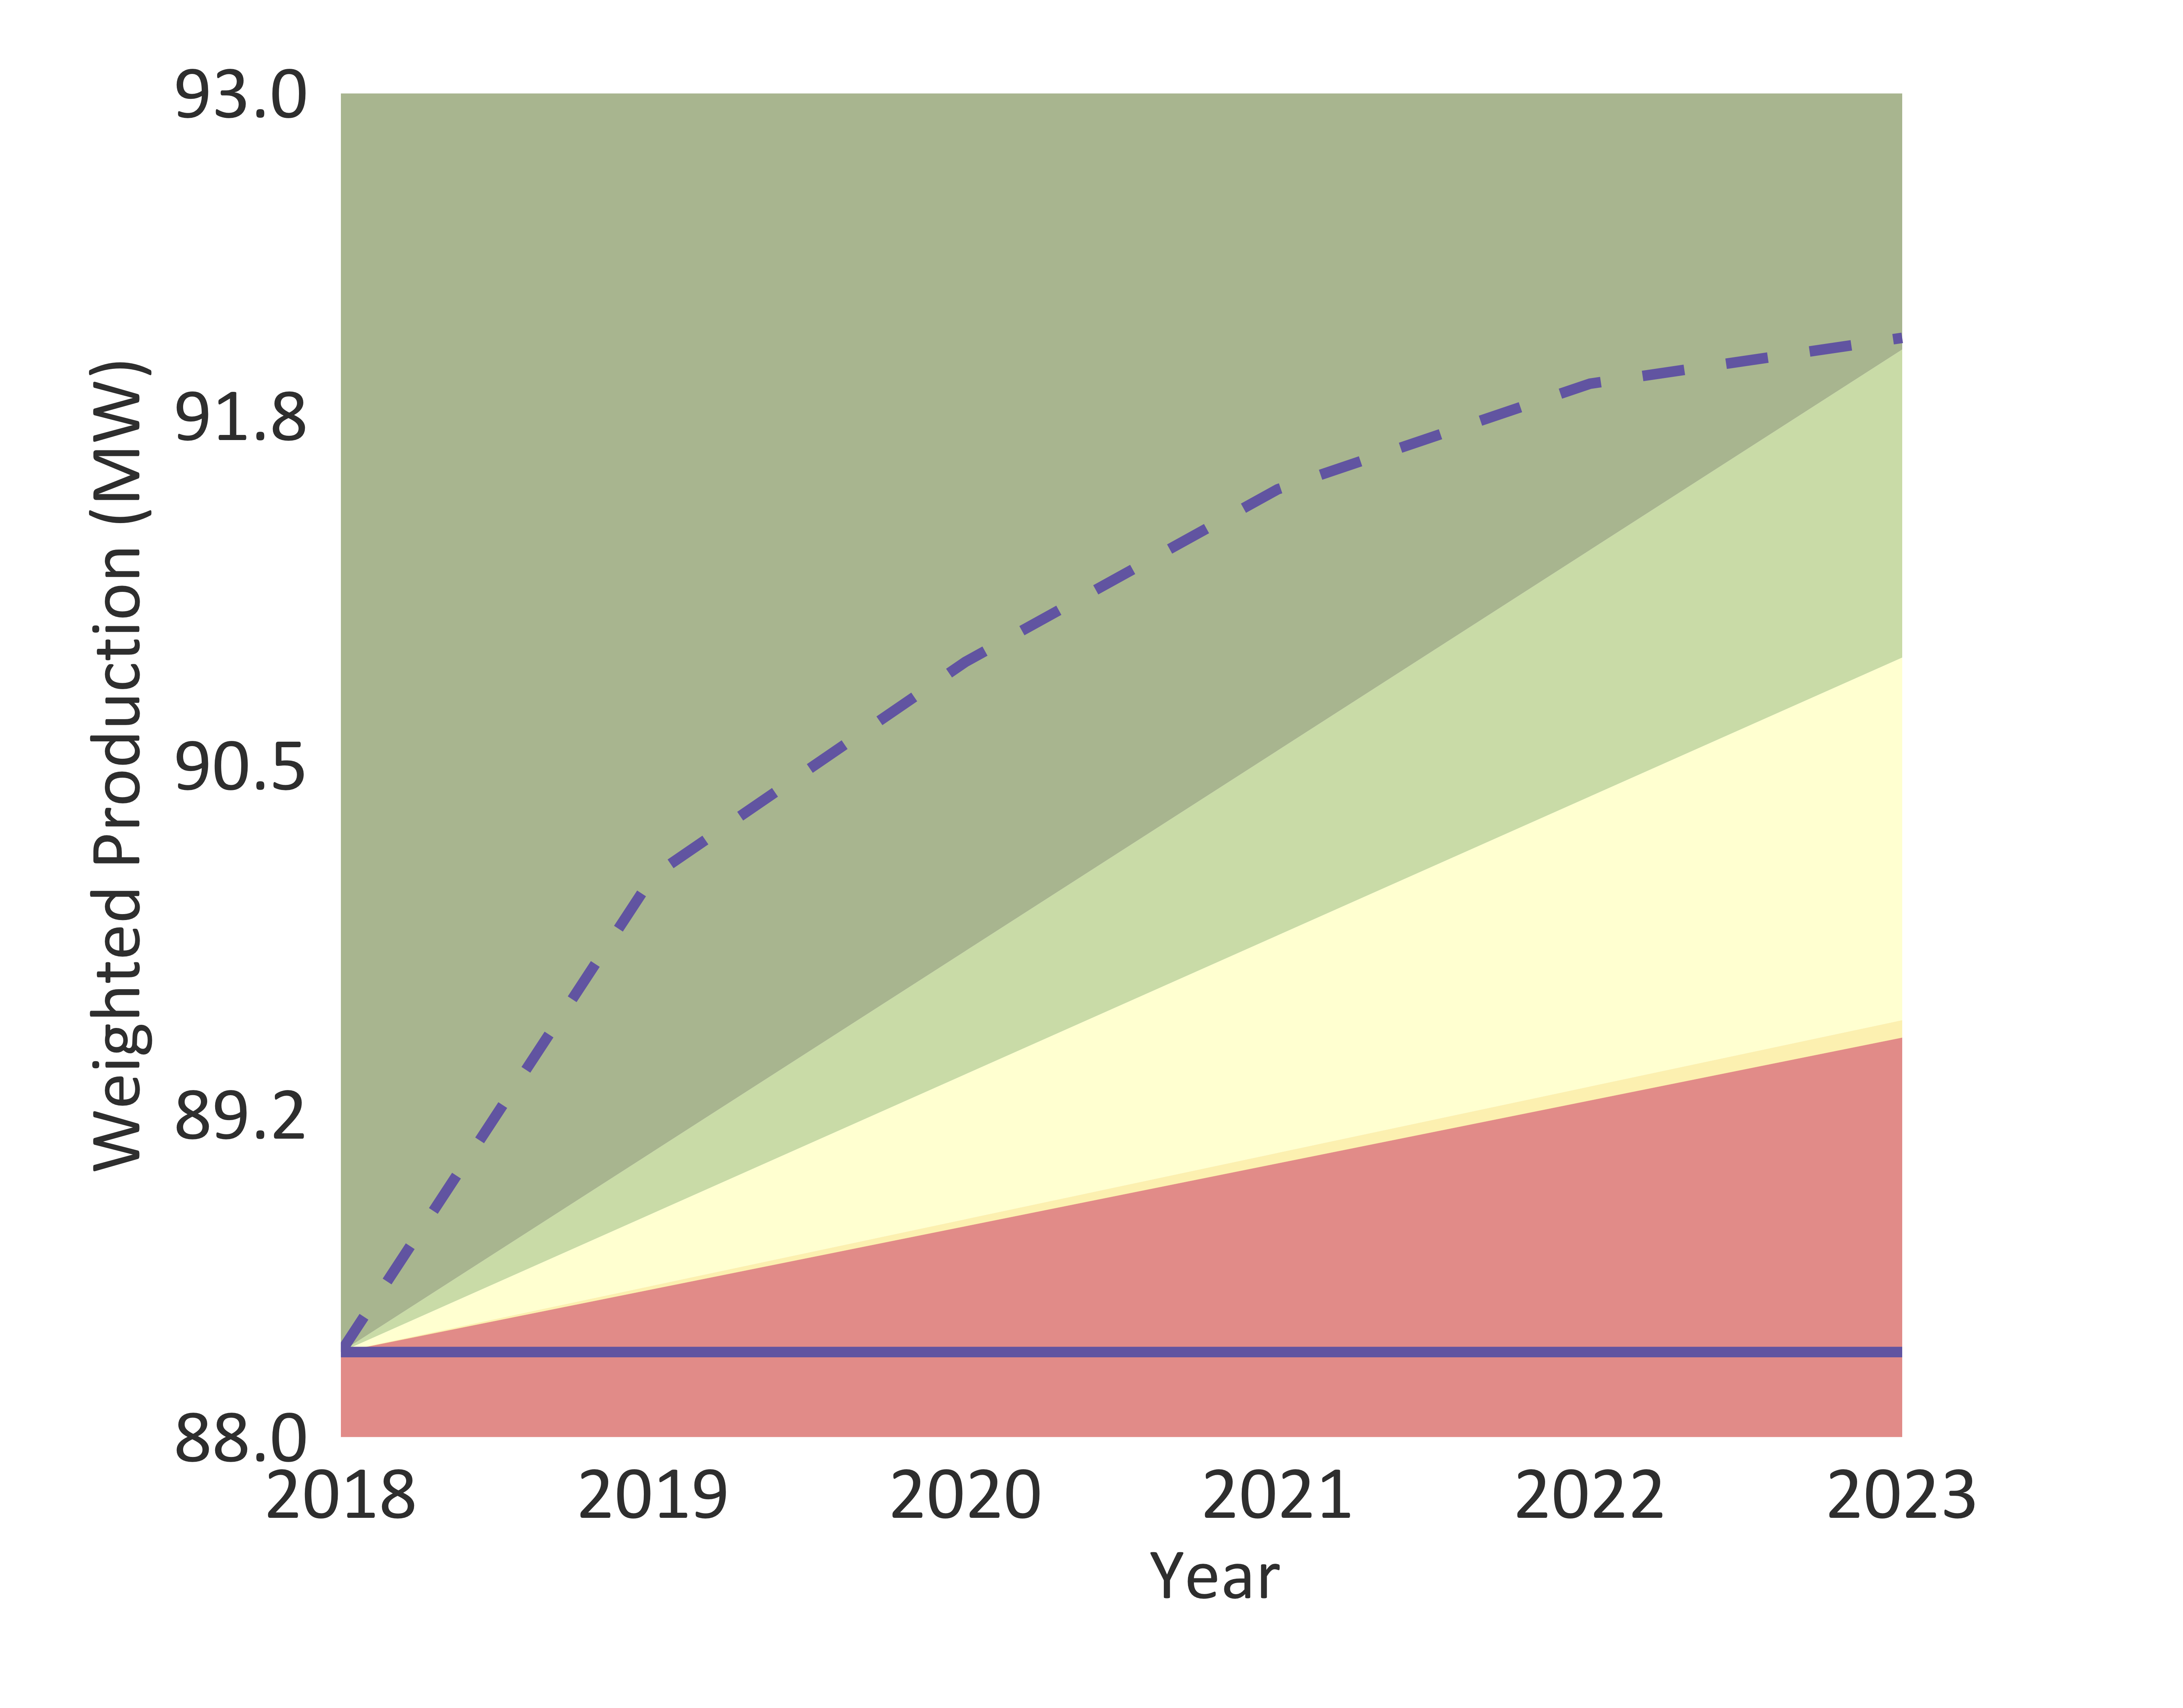
\includegraphics[trim = {0 0cm 0 0},width=1\linewidth]{CAFigures/Fig10}
		
		\textbf{Growth in Gas Power Capacity }
		
		Ranking: EQGasCapRank
		
		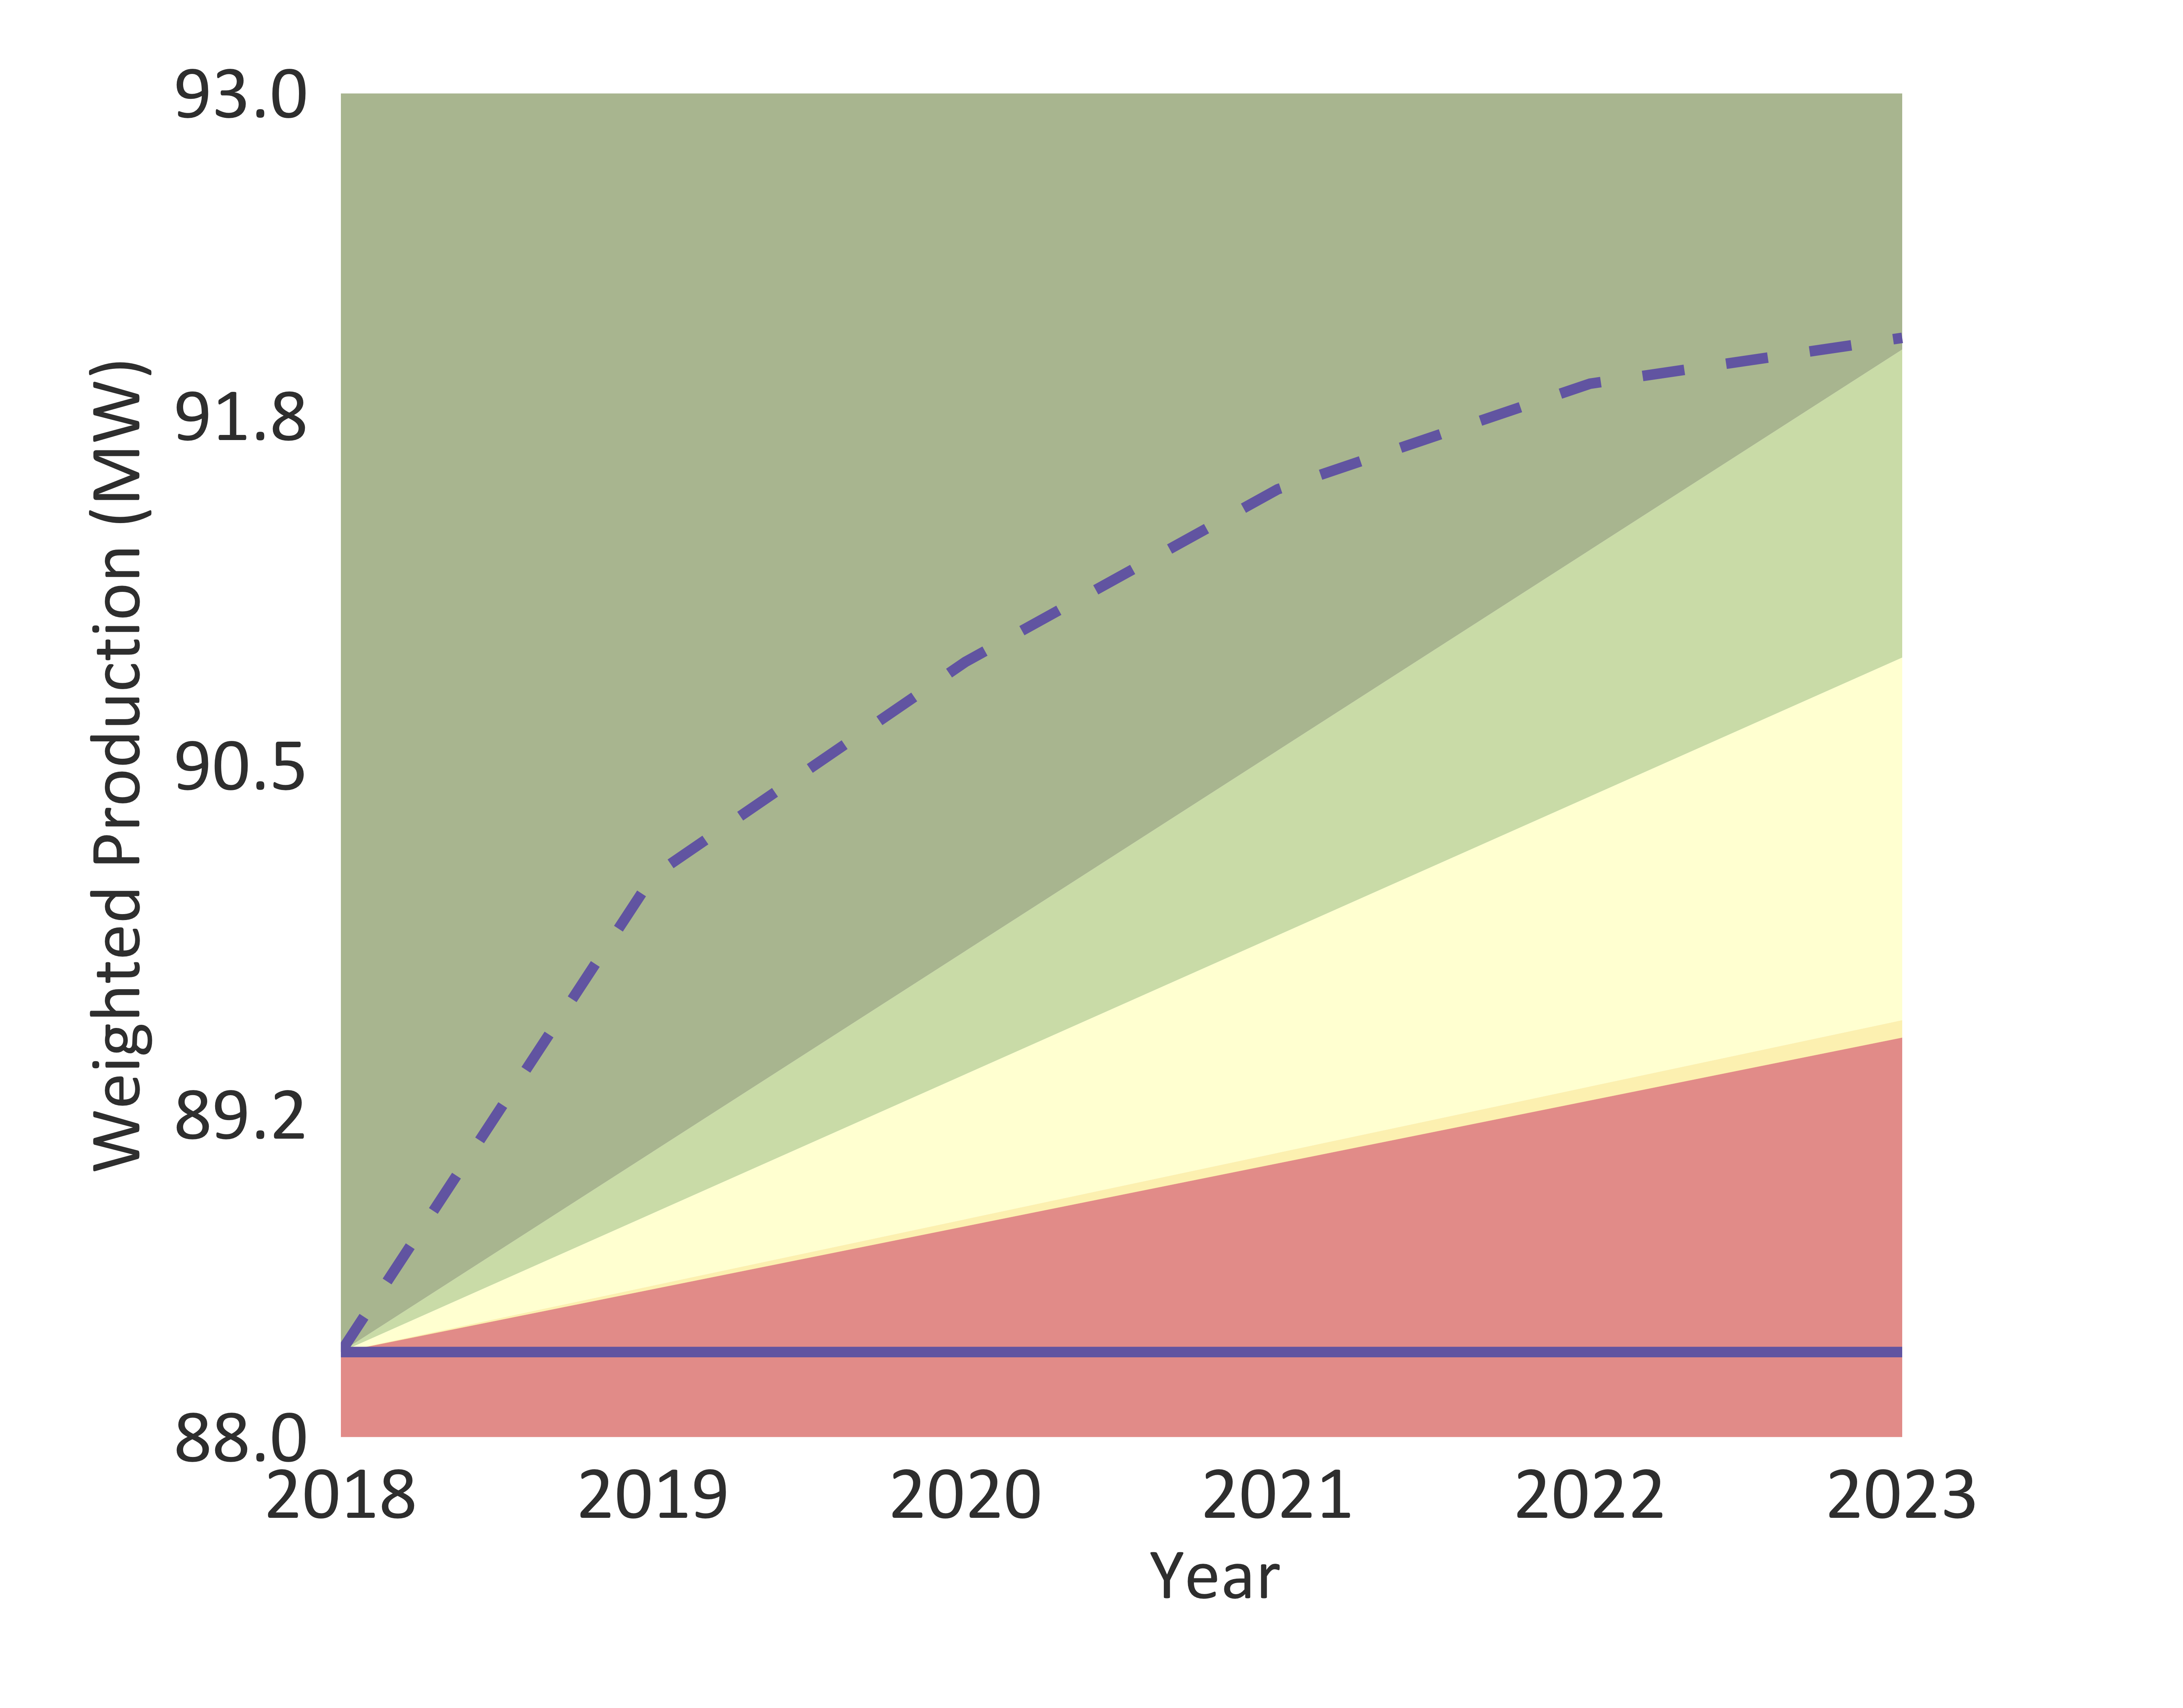
\includegraphics[trim = {0 0cm 0 0},width=1\linewidth]{CAFigures/Fig10}
	\end{minipage}	
	\hspace{.02\linewidth}
	\begin{minipage}[t]{.49\textwidth}
		\textbf{Growth in Renewable Power Capacity }
		
		Ranking: EQRenewableCapRank
		
		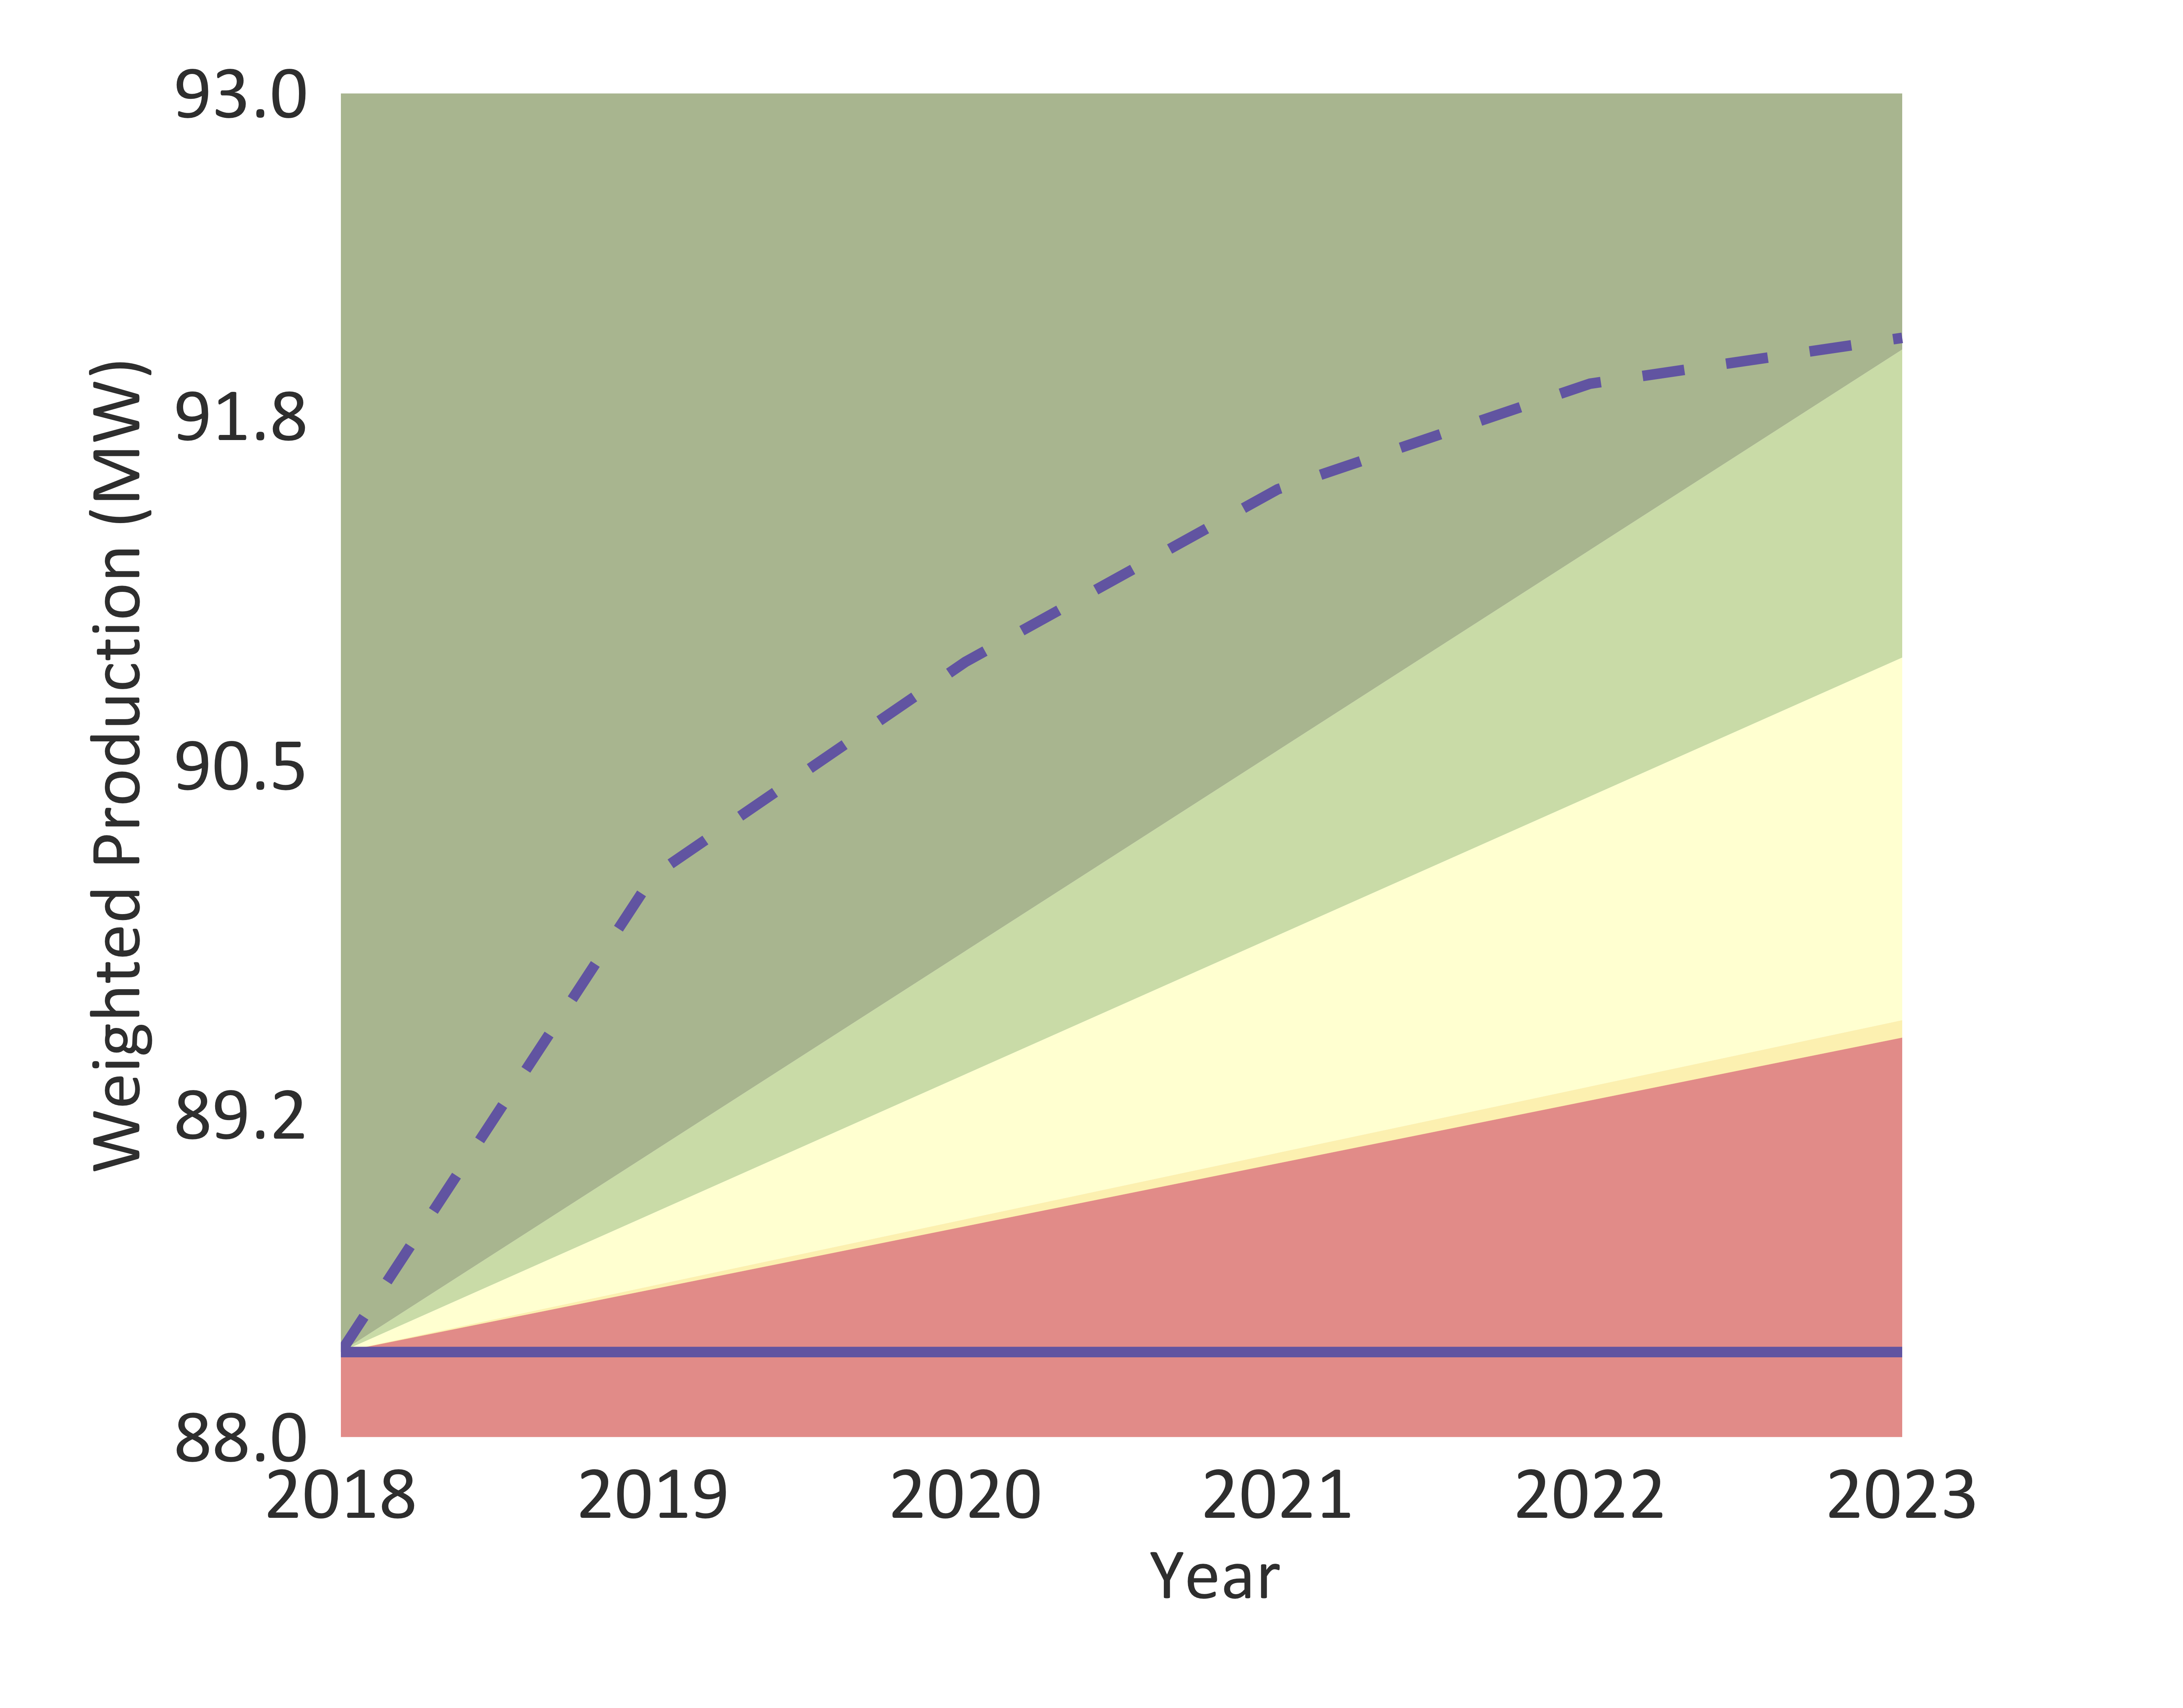
\includegraphics[trim = {0 0cm 0 0},width=1\linewidth]{CAFigures/Fig10}
		\textbf{Growth in Nuclear Power Capacity }
	
		Ranking:EQNuclearCapRank
		
		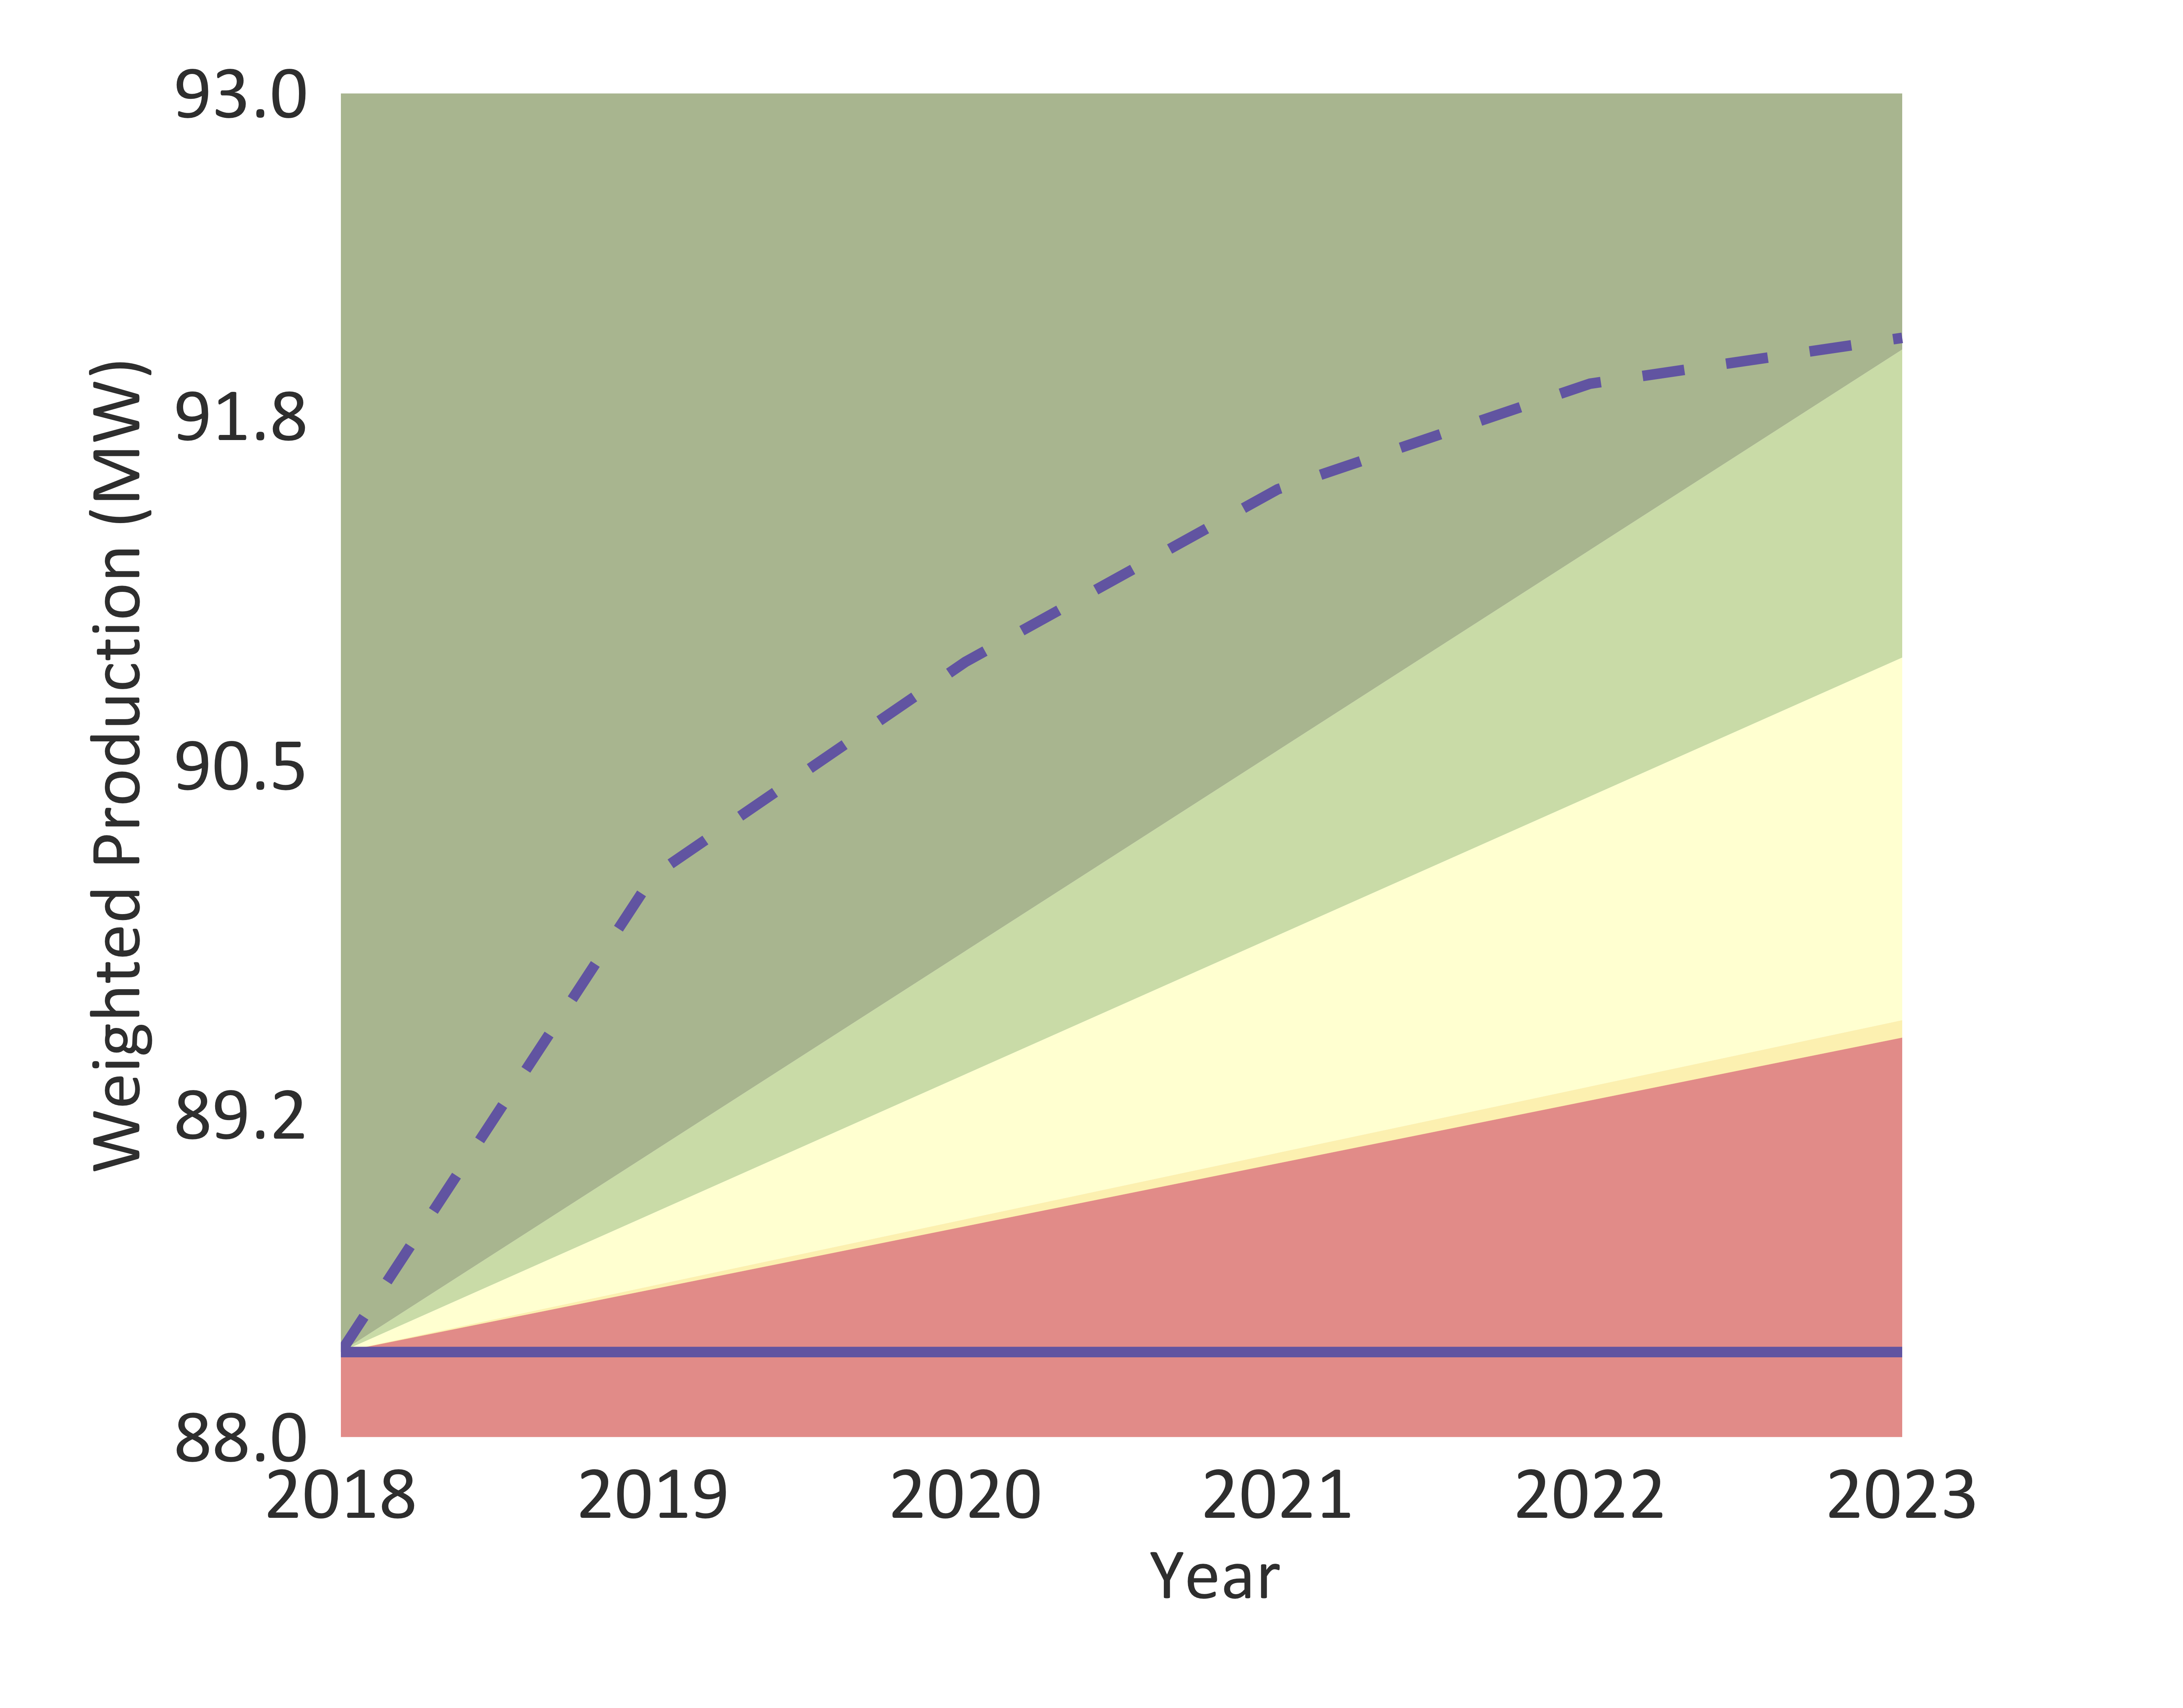
\includegraphics[trim = {0 0cm 0 0},width=1\linewidth]{CAFigures/Fig10}
	\end{minipage}
	
	\newpage	
	\section*{P12} % TRAJECTORY – EQUITY – FOSSIL FUELS AND AUTOMOTIVE
	\PageHeading{TRAJECTORY – EQUITY – FOSSIL FUELS AND AUTOMOTIVE
	}		
	
	\textbf{The alignment graphs below show the alignment of selected fossil fuels and automobile technologies in your portfolio relative to the IEA scenarios for 2°C, 4°C and 6°C temperature change, the global stock market and the average of your peers. } 
	
	The page brings together data on the upstream supply of fossil fuels and the largest downstream user of oil, namely the automotive sector. It highlights the extent to which within a portfolio the strategies across sectors may be more or less consistent, relative to a 2°C scenario.
	 
	
	\vspace{1cm}
	
	\begin{center}
		\textbf{OIL AND GAS}
	\end{center}
	
	\begin{minipage}[t]{.49\linewidth}
		\textbf{Growth in Oil Production }
		
		Ranking: EQOilRank
		
		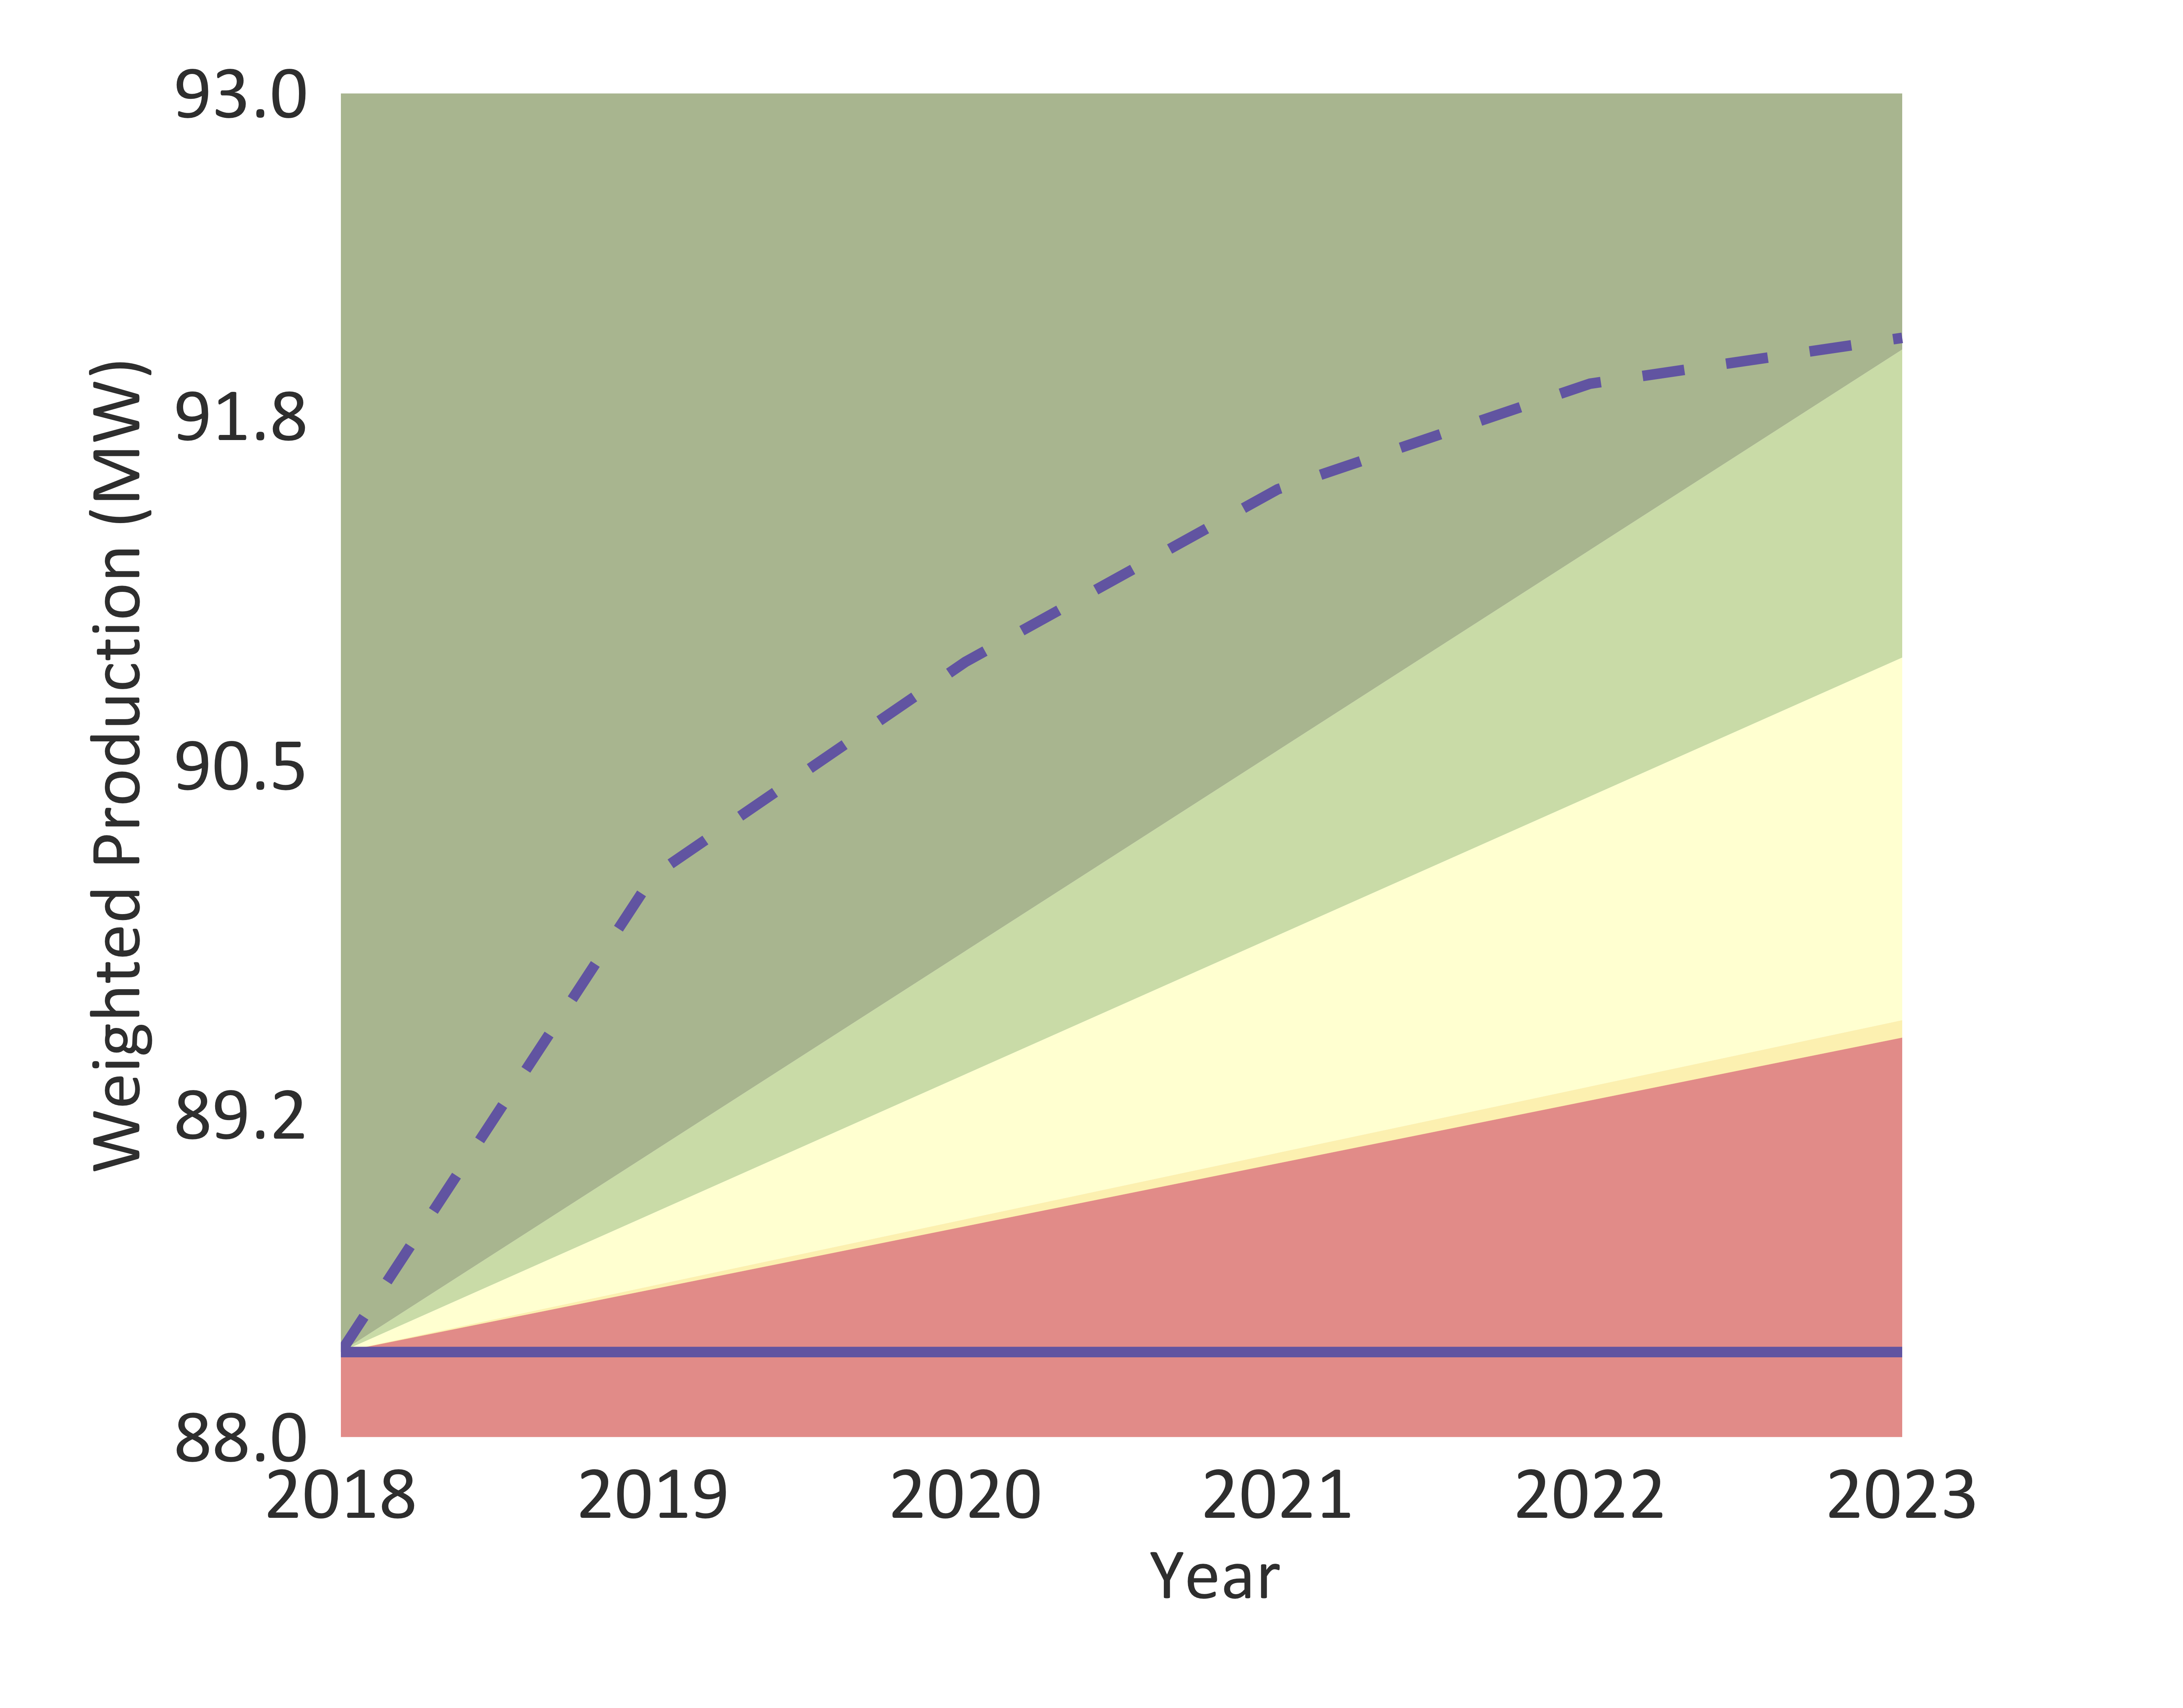
\includegraphics[trim = {0 0cm 0 0},width=1\linewidth]{CAFigures/Fig10}
		
	\end{minipage}	
	\hspace{.02\linewidth}
	\begin{minipage}[t]{.49\textwidth}
		\textbf{Growth in Gas Production }
		
		Ranking: EQGasRank
		
		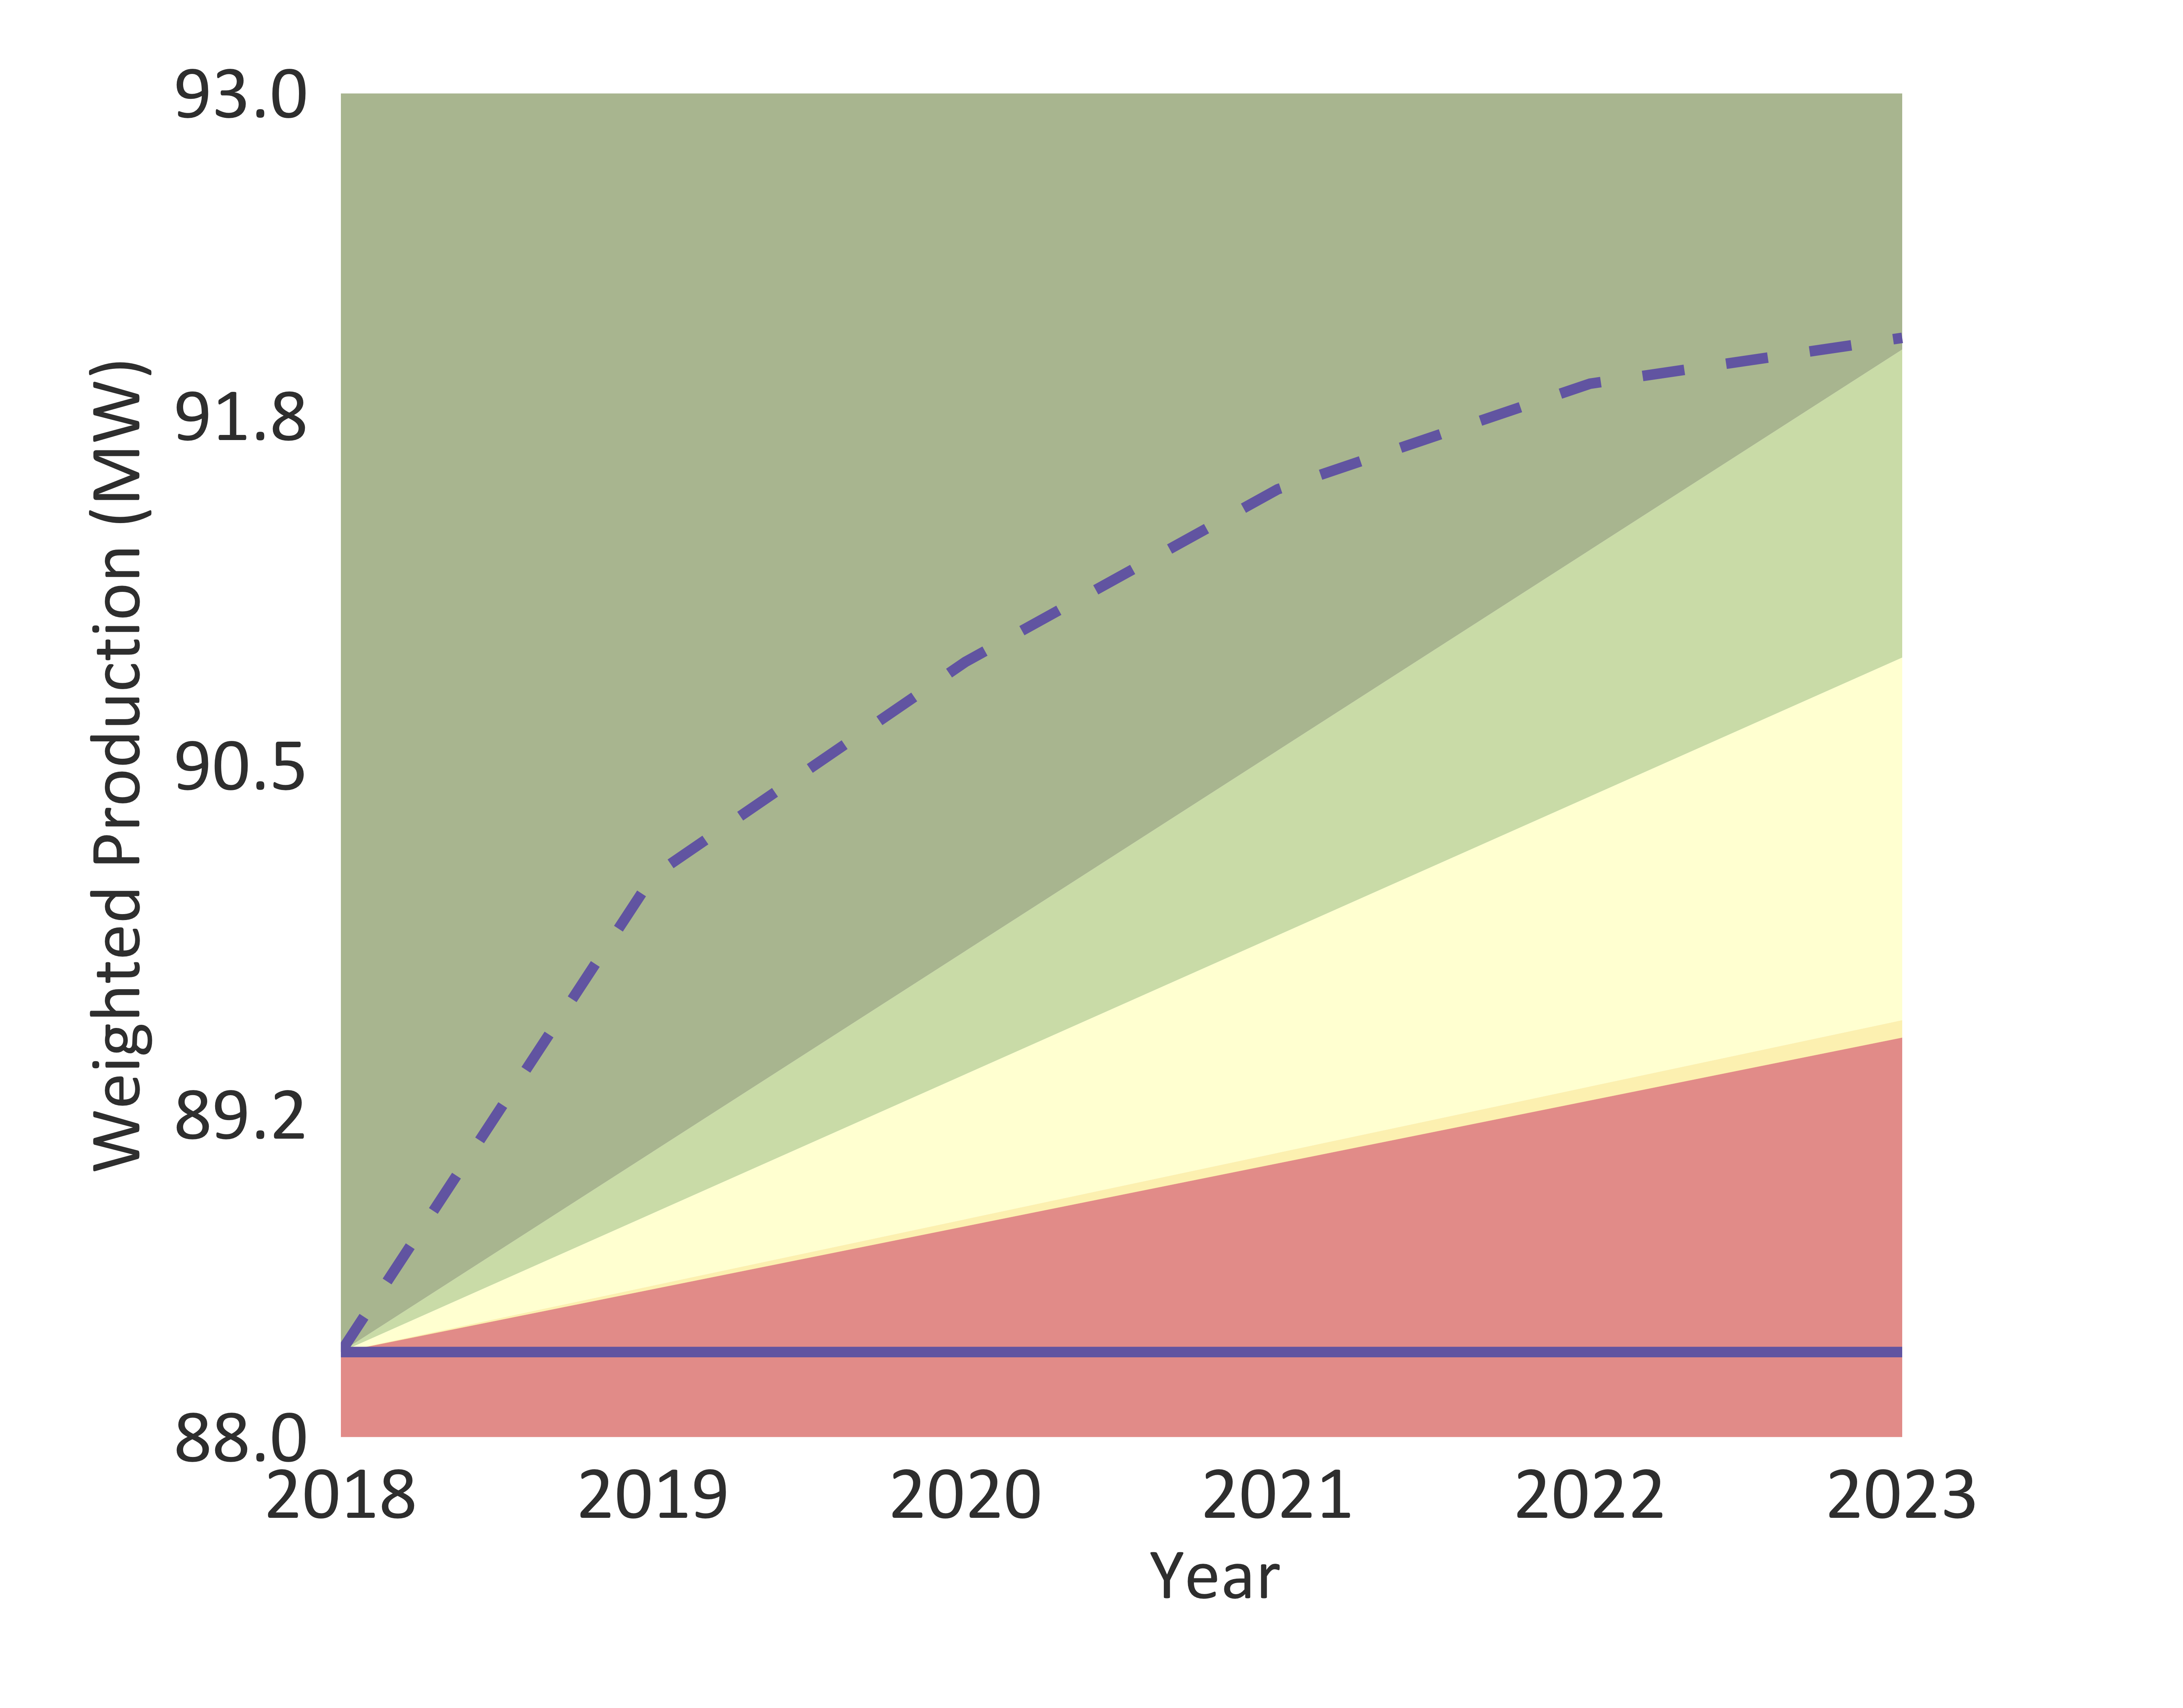
\includegraphics[trim = {0 0cm 0 0},width=1\linewidth]{CAFigures/Fig10}

	\end{minipage}


	\begin{center}
		\textbf{AUTOMOBILE PRODUCTION}
	\end{center}
	
	\begin{minipage}[t]{.49\linewidth}
		\textbf{Growth in Combustion Engine Vehicle Production}
		
		Ranking: EQICERank
		
		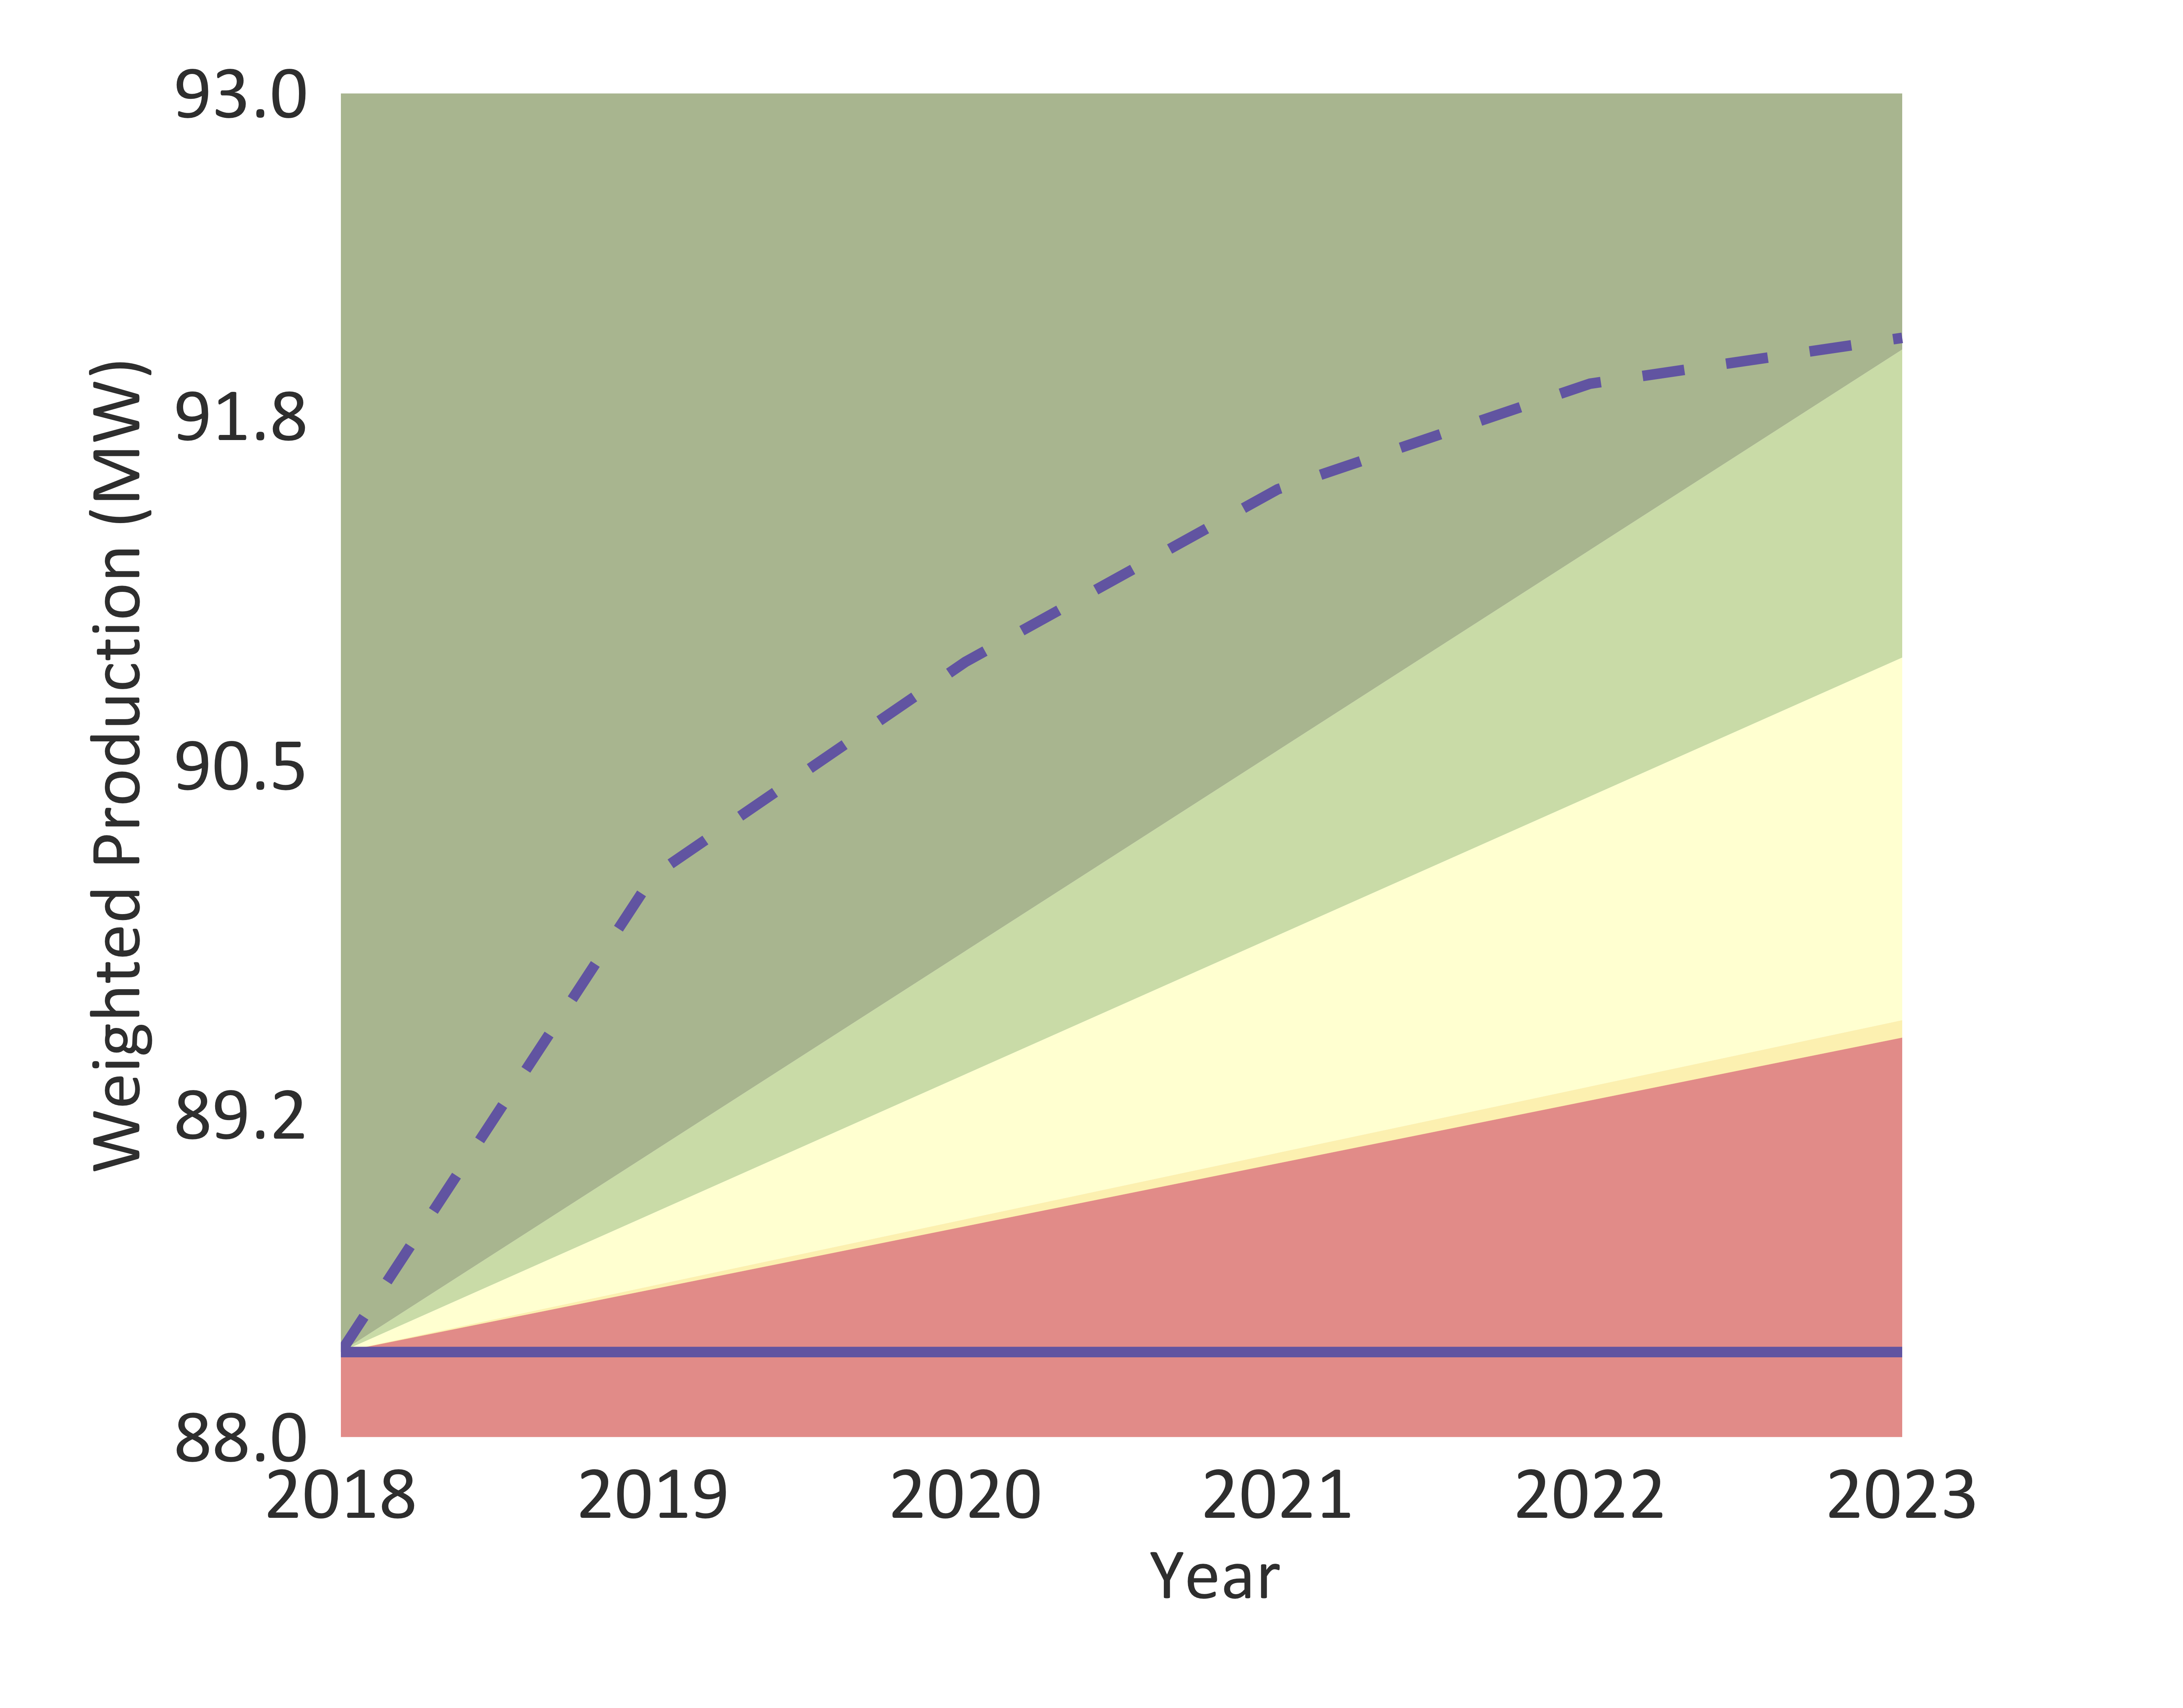
\includegraphics[trim = {0 0cm 0 0},width=1\linewidth]{CAFigures/Fig10}
		
	\end{minipage}	
	\hspace{.02\linewidth}
	\begin{minipage}[t]{.49\textwidth}
		\textbf{Growth in Electric Vehicle Production}
		
		Ranking: EQElectricRank
		
		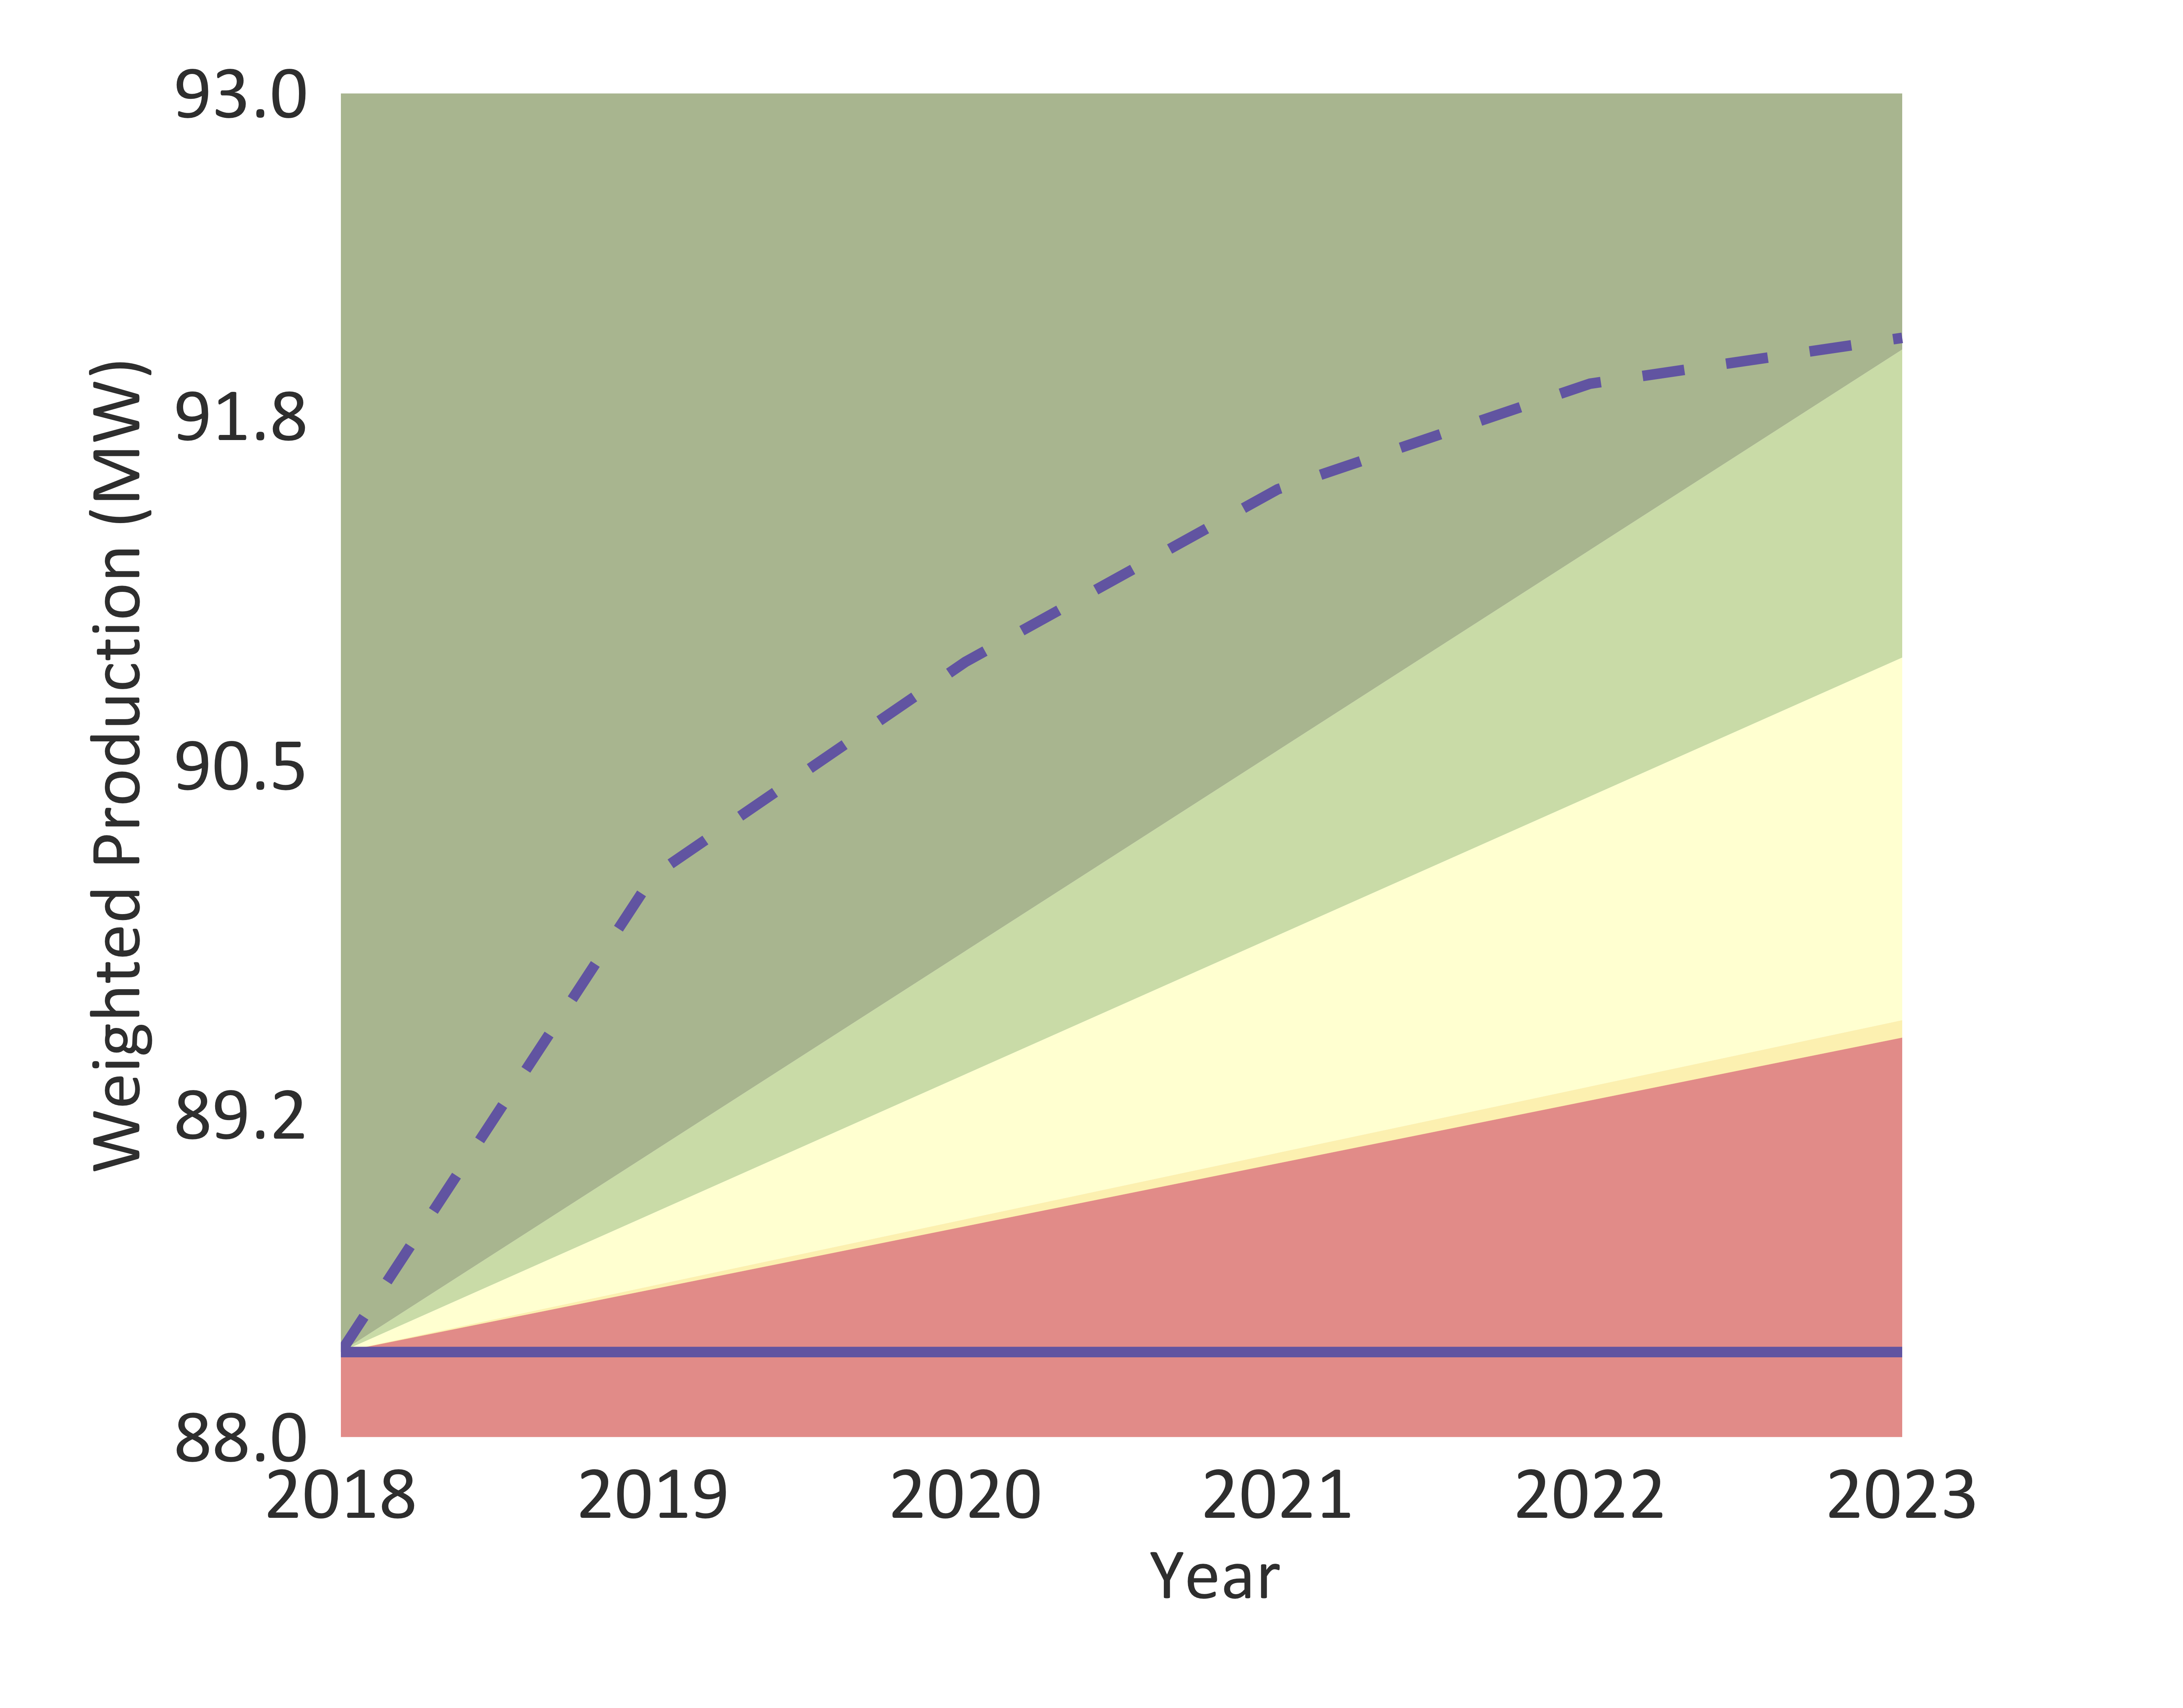
\includegraphics[trim = {0 0cm 0 0},width=1\linewidth]{CAFigures/Fig10}
		
	\end{minipage}		
		
		
		
	\newpage	
	\section*{P15} % 3rd Section
	\thispagestyle{empty}
	\vspace{17cm}
	\SectionHeading{Section 4:}{THE EXPOSURE OF YOUR PORTFOLIO TO 2°C SCENARIOS IN 2023}
	
	
	\newpage	
	\section*{P16} % FUTURE EXPOSURE – 2023 – LISTED EQUITY
	\PageHeading{FUTURE EXPOSURE – 2023 – LISTED EQUITY}
		
	\textbf{The figure below shows the estimated exposure of your listed equity portfolio in 2023 to the technologies and fuels in the climate relevant sectors covered in this analysis. }
		
	The results are a function both of the starting point of the exposure (Section 2) and the evolution of the exposure over time (Section 3) based on current revealed investment and production plans for all technologies. The results show the relative exposure of your portfolios across asset classes and technologies / fuels. They should be interpreted as follows:
	
	\begin{itemize}
		\item{100\% alignment suggests the portfolio weights the respective technology / fuel identically to the market in 2023 – freezing both the current portfolio exposure and the current revealed production / investment plans of companies within those portfolios.}
		
		\item{Any figure above 100\% suggests that the portfolio ‘exceeds’ the expected market exposure under a 2°C transition. This implies a higher exposure to low-carbon technologies (marked as green) and a lower exposure to high-carbon technologies (marked as black). Thus, a figure of 110\% for oil production implies an under-weight of oil production relative to the 2°C benchmark of 10\%. }
		
	\end{itemize}	

	\begin{center}
		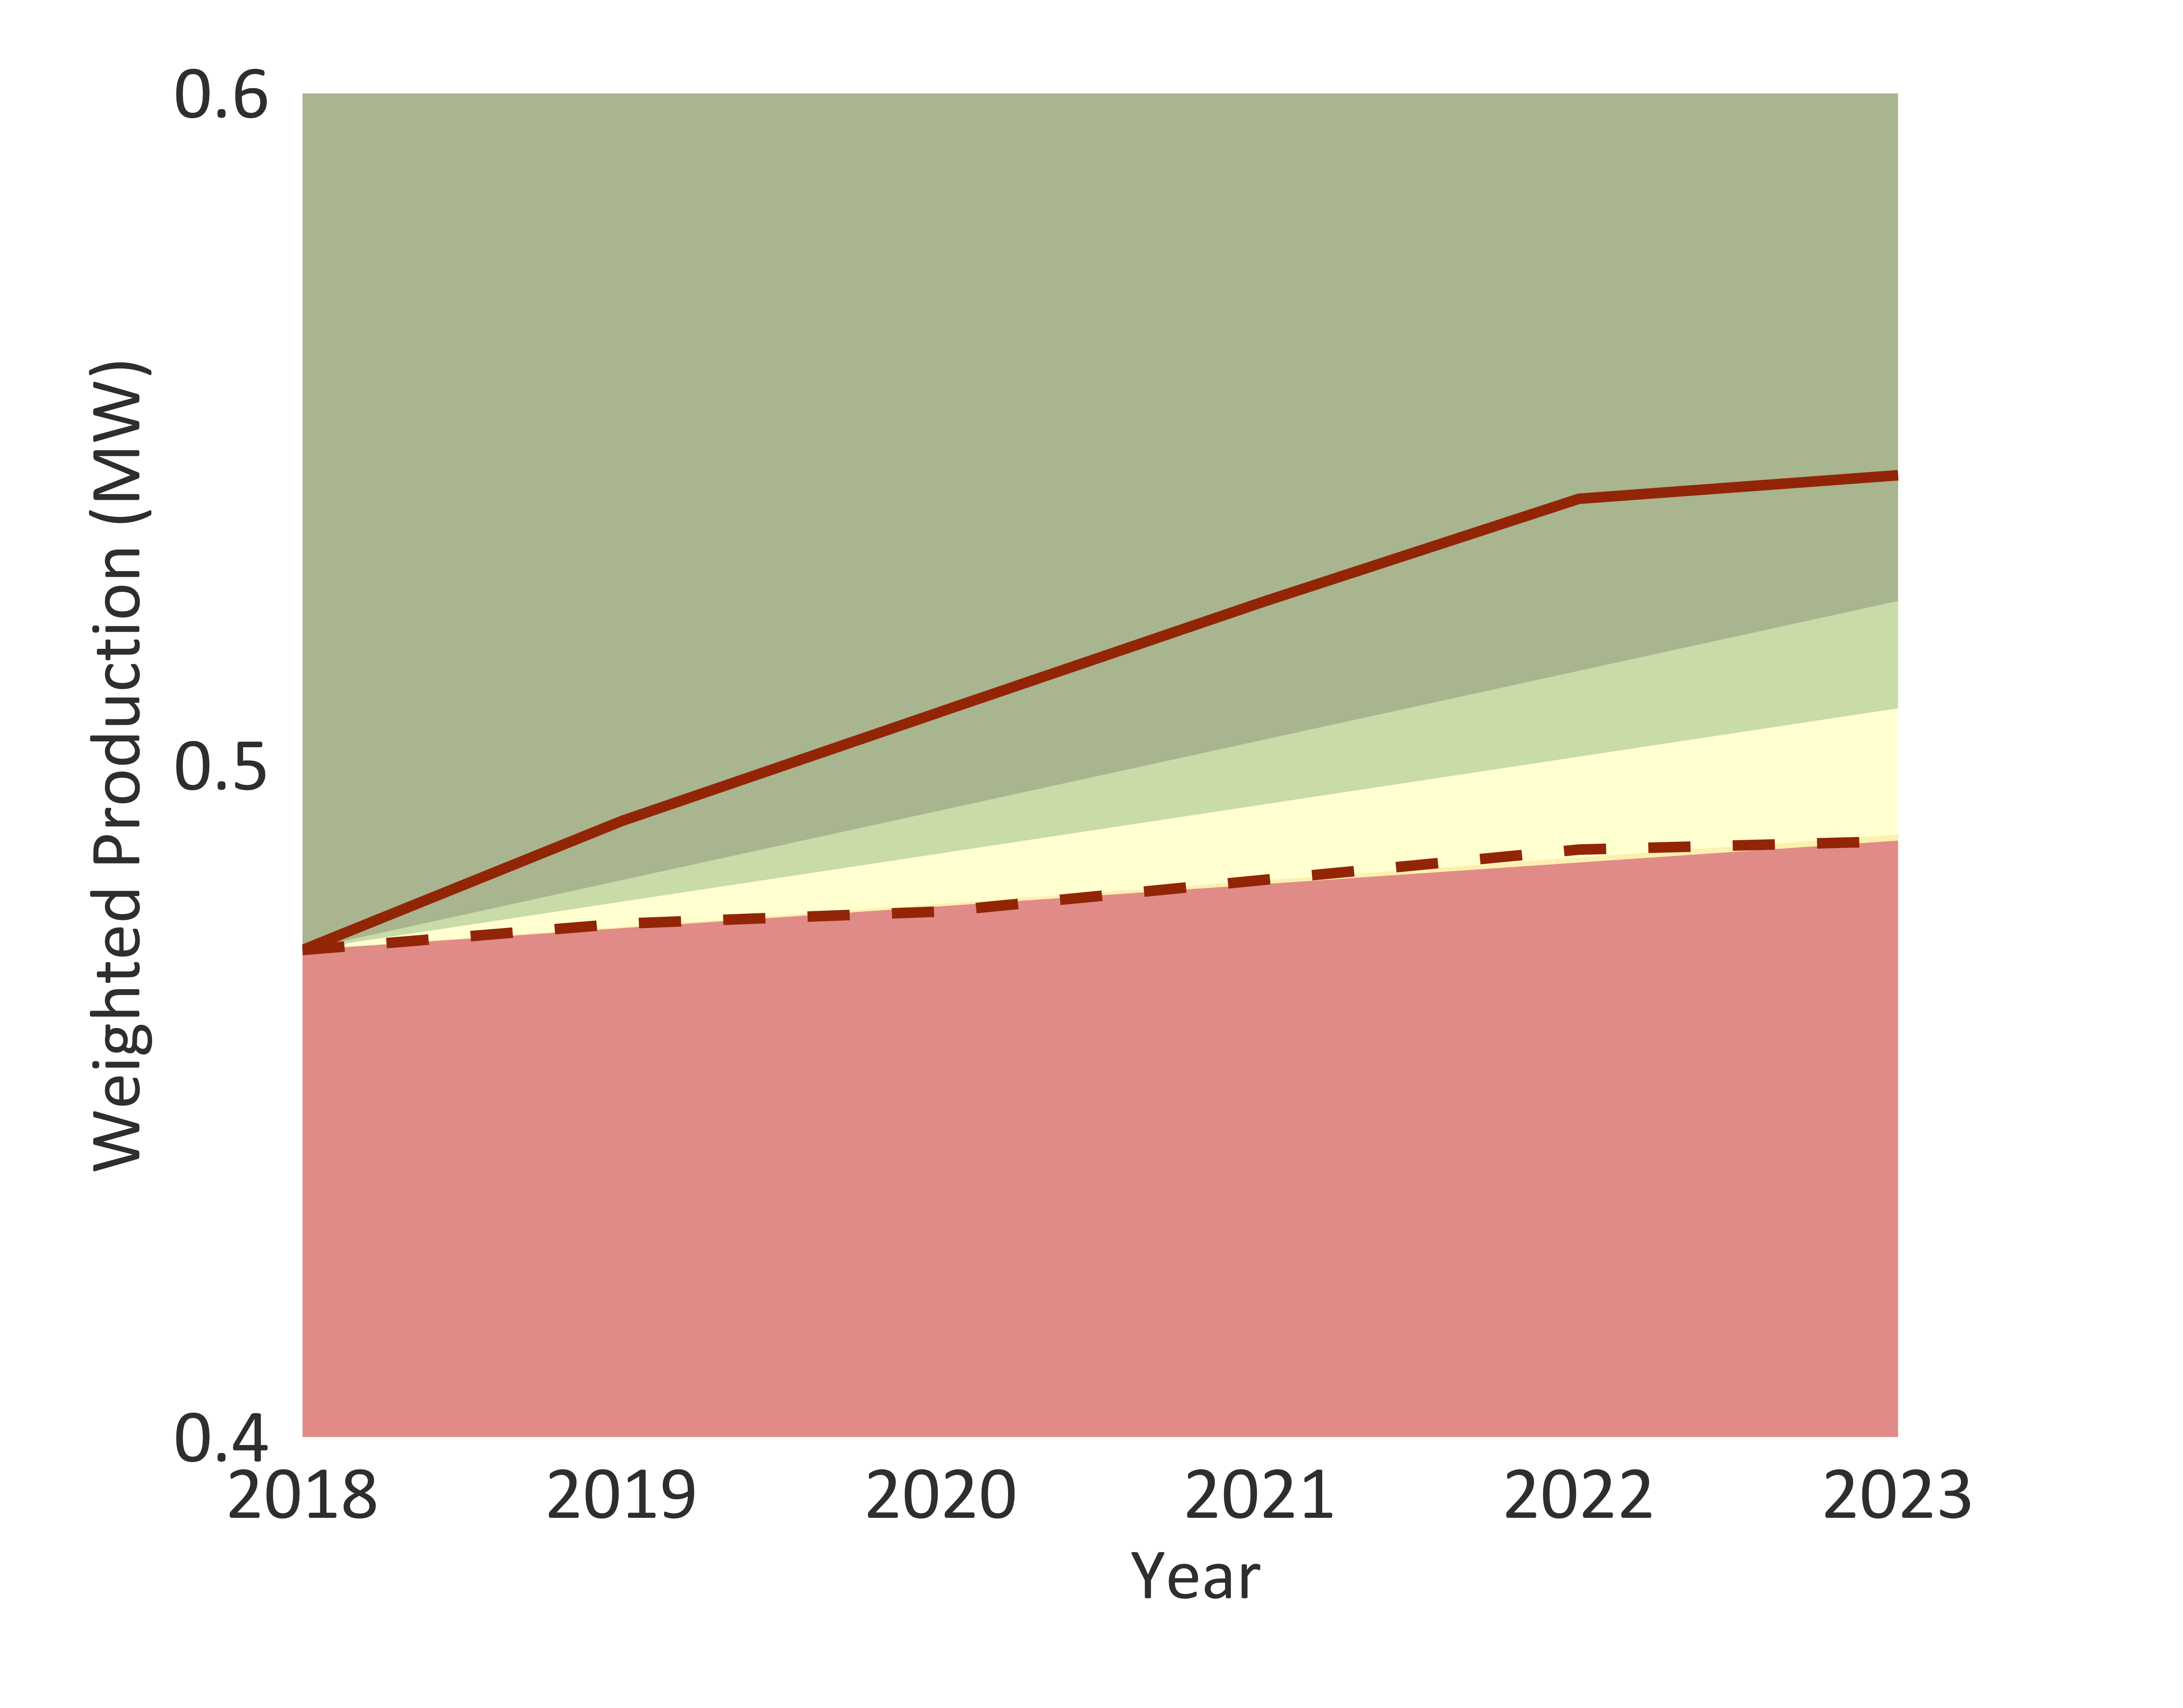
\includegraphics[trim = {0 0cm 0 0},width=.75\linewidth]{CAFigures/Fig20}
	\end{center}
	

	\newpage
	\section*{P17} % FUTURE EXPOSURE – 2023 – CORPORATE BONDS
	\PageHeading{FUTURE EXPOSURE – 2023 – CORPORATE BONDS}
	
	\textbf{The figure below shows the estimated exposure of your listed equity portfolio in 2023 to the technologies and fuels in the climate relevant sectors covered in this analysis. }
	
	The results are a function both of the starting point of the exposure (Section 2) and the evolution of the exposure over time (Section 3) based on current revealed investment and production plans for all technologies. The results show the relative exposure of your portfolios across asset classes and technologies / fuels. They should be interpreted as follows:
	
	\begin{itemize}
		\item{100\% alignment suggests the portfolio weights the respective technology / fuel identically to the market in 2023 – freezing both the current portfolio exposure and the current revealed production / investment plans of companies within those portfolios.}
		
		\item{Any figure above 100\% suggests that the portfolio ‘exceeds’ the expected market exposure under a 2°C transition. This implies a higher exposure to low-carbon technologies (marked as green) and a lower exposure to high-carbon technologies (marked as black). Thus, a figure of 110\% for oil production implies an under-weight of oil production relative to the 2°C benchmark of 10\%. }
		
	\end{itemize}	
	
	\begin{center}
		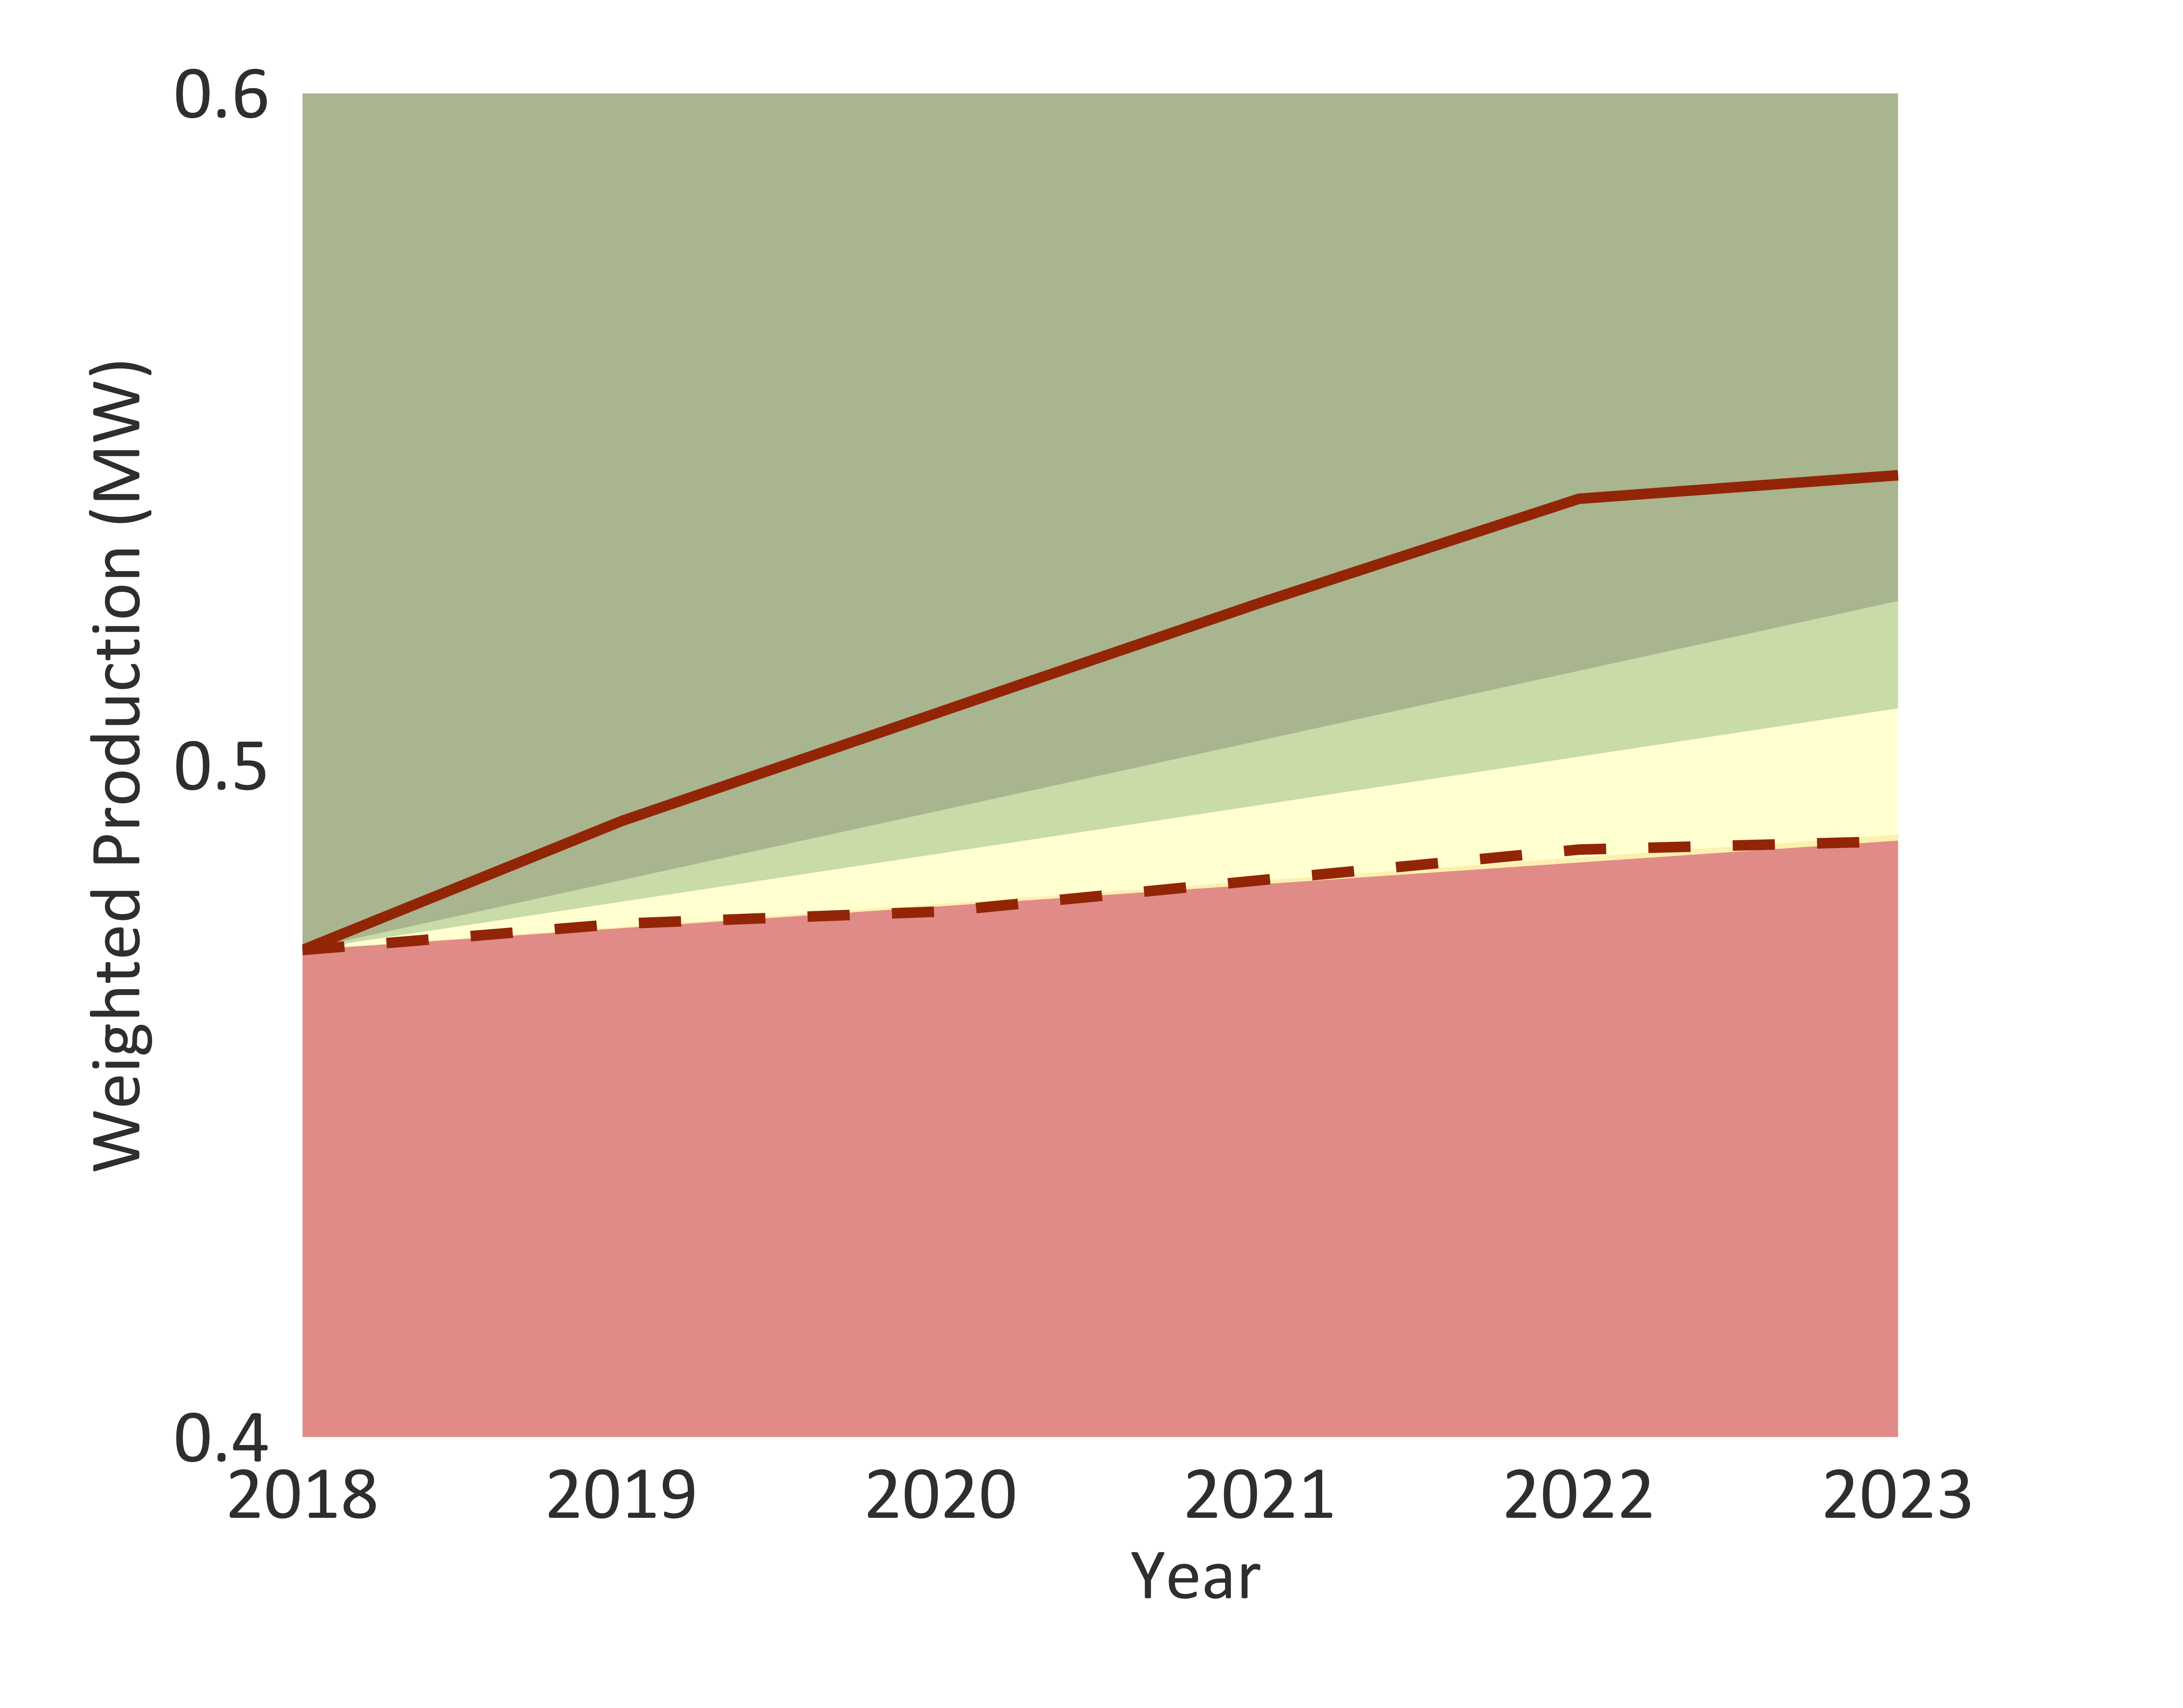
\includegraphics[trim = {0 0cm 0 0},width=.75\linewidth]{CAFigures/Fig20}
	\end{center}
	
	\newpage	
	\section*{P18} % Company Exposure
	\thispagestyle{empty}
	\vspace{17cm}
	\SectionHeading{Section 5:}{COMPANY EXPOSURE}
	
	\newpage
	\section*{P19} % CONTRIBUTIONS OF SECURITIES TO THE RESULTS - POWER
	\PageHeading{CONTRIBUTIONS OF SECURITIES TO THE RESULTS}
	
	The following chart shows the technology mix of Power companies within your portfolio and the stock market. From the accounting principles applied in this test, a portion of capacity from each company has been allocated to your portfolio based on your ownership. The following lists identify the largest contributors by technology identifying both the absolute capacity allocated to your portfolio and what percent of the total capacity of your portfolio this accounts for in 2023. 
	
	This information is valid for your equity portfolio. 
	
	\begin{center}
		\textbf{POWER COMPANIES}
		
		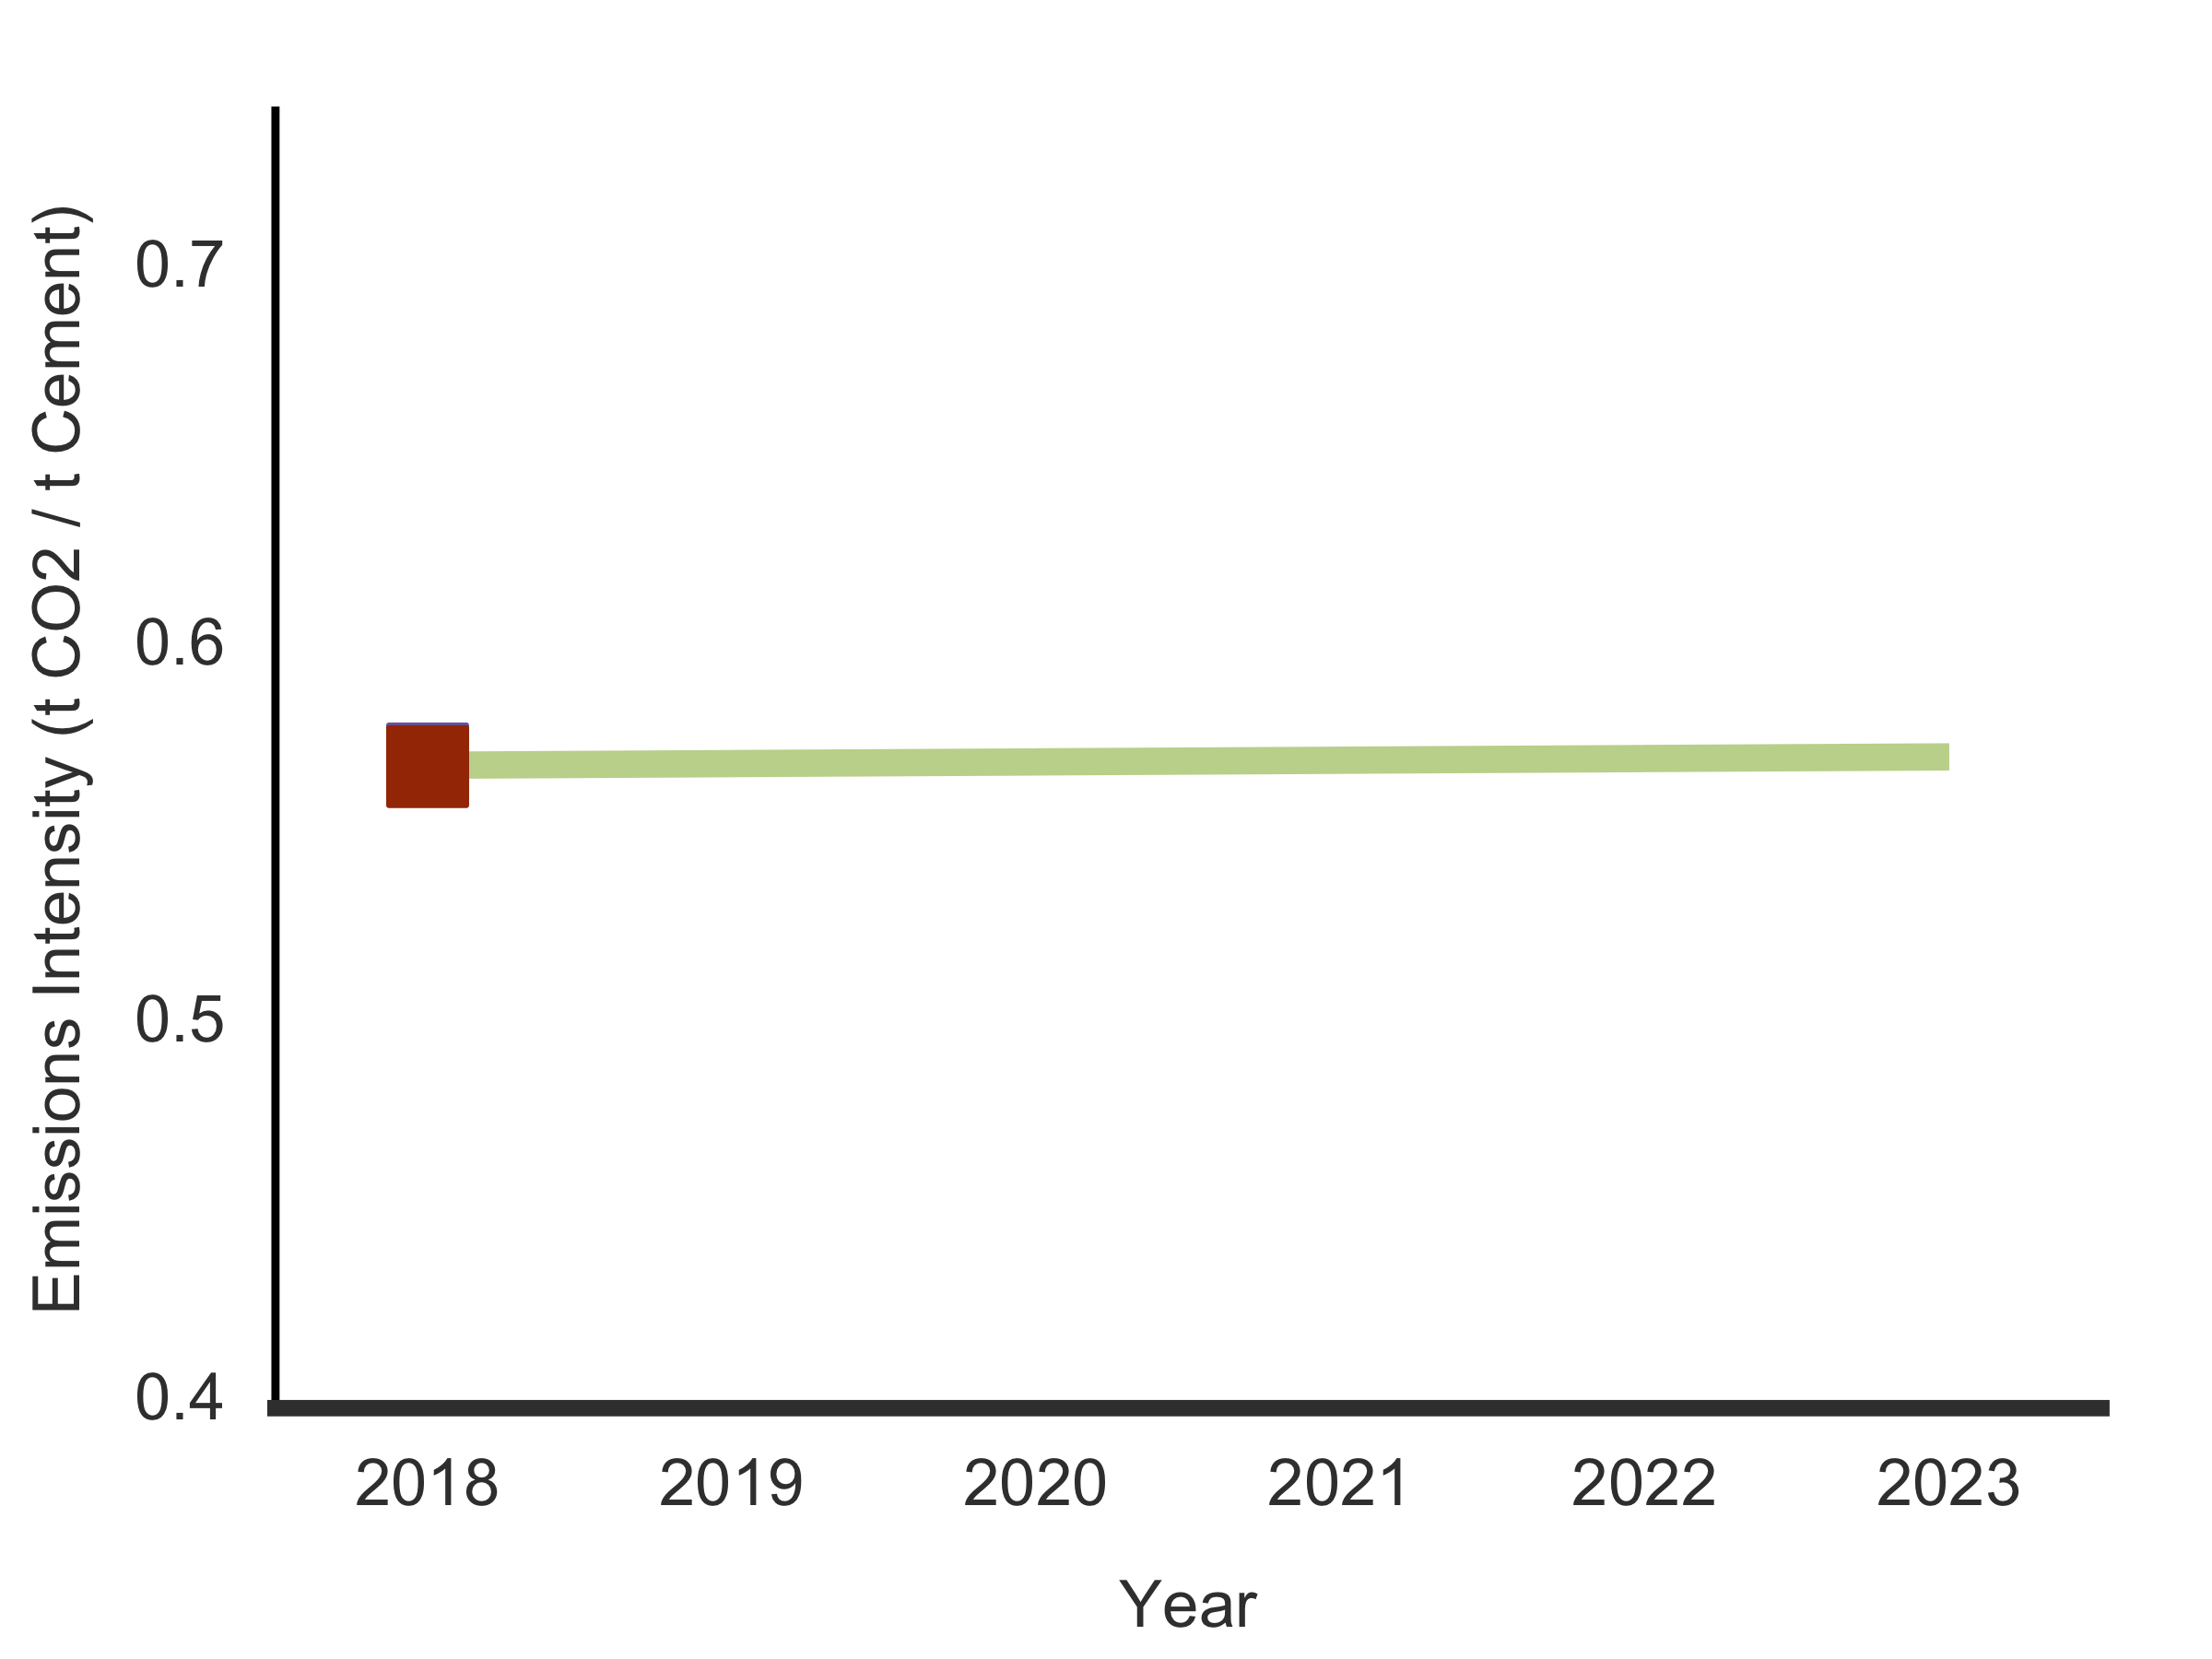
\includegraphics[trim = {0 0cm 0 0},width=1\linewidth]{CAFigures/Fig30}
	\end{center}

	\newpage
	\section*{P20} % CONTRIBUTIONS OF SECURITIES TO THE RESULTS - POWER
	\PageHeading{CONTRIBUTIONS OF SECURITIES TO THE RESULTS}
	
	The following chart shows the technology mix of Automotive companies within your portfolio and the stock market. From the accounting principles applied in this test, a portion of production from each company has been allocated to your portfolio based on your ownership. The following lists identify the largest contributors by technology identifying both the absolute production allocated to your portfolio and what percent of the total capacity of your portfolio this accounts for in 2023. 
	
	
	This information is valid for your equity portfolio. 
	
	\begin{center}
		\textbf{AUTOMOTIVE COMPANIES}
		
		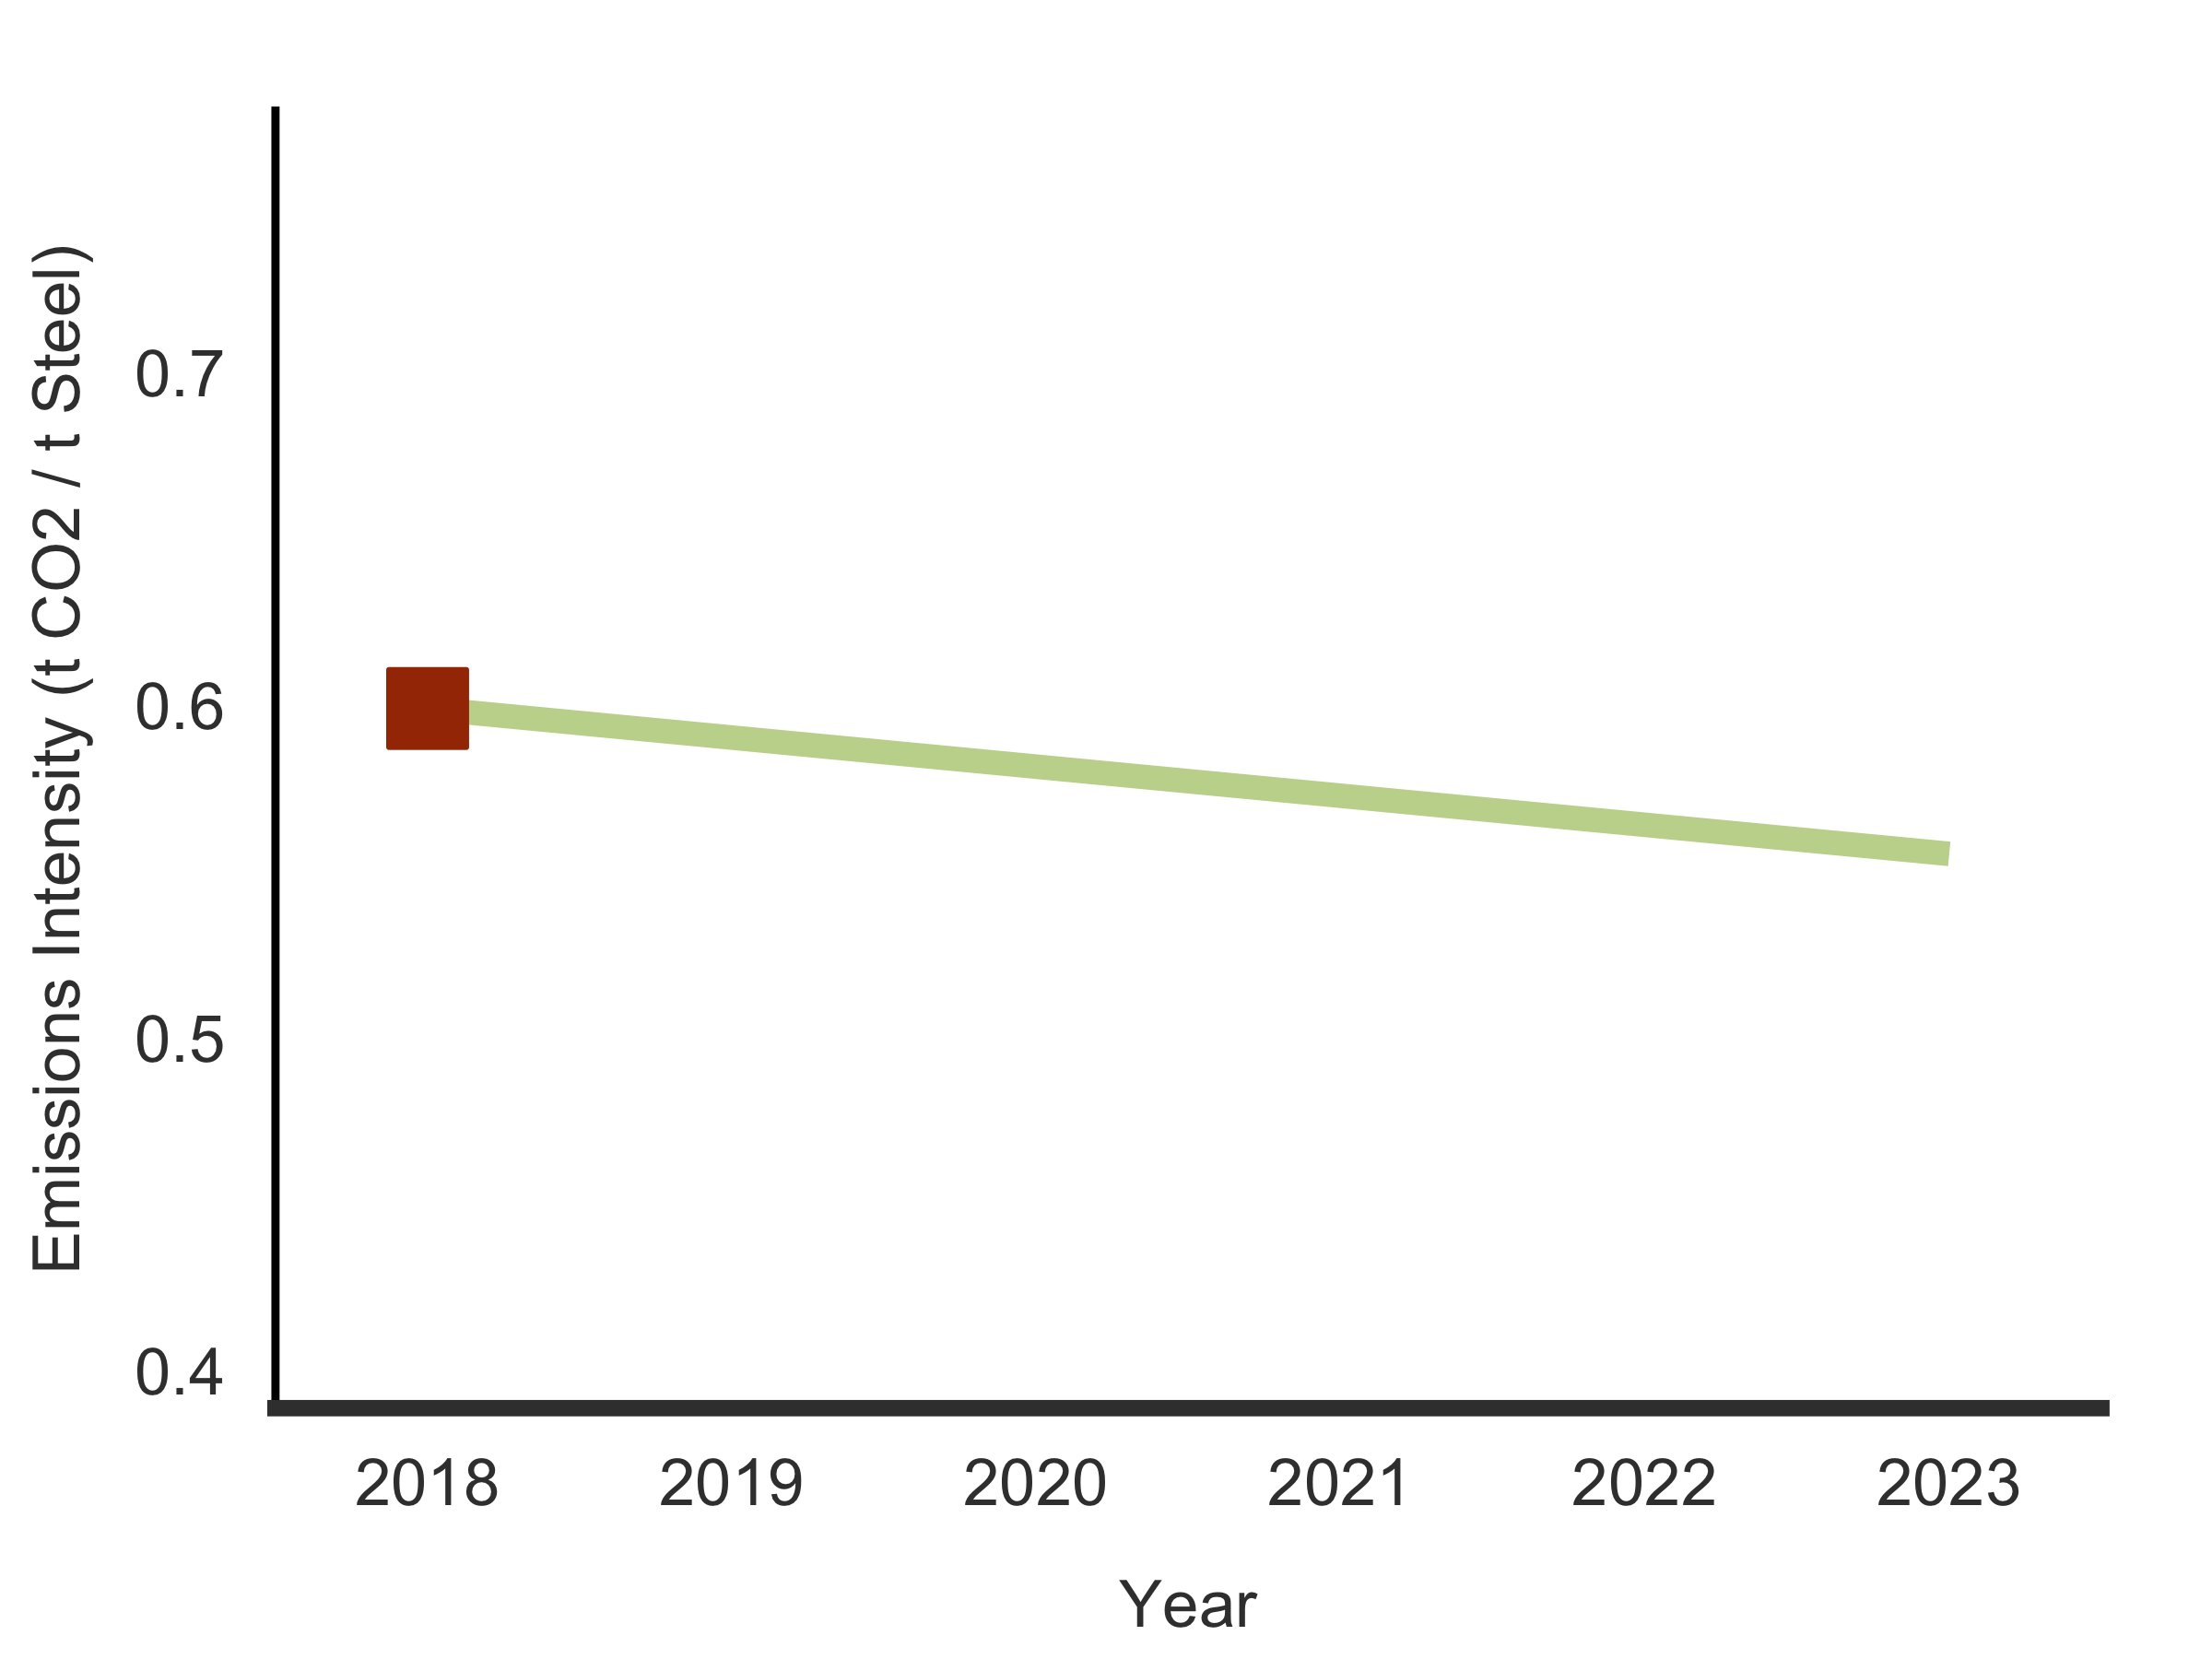
\includegraphics[trim = {0 0cm 0 0},width=1\linewidth]{CAFigures/Fig31}
	\end{center}


	\newpage
\section*{P21} % CONTRIBUTIONS OF SECURITIES TO THE RESULTS - POWER
\PageHeading{CONTRIBUTIONS OF SECURITIES TO THE RESULTS}

On this basis, the share of reserves/future production which is outside the 2°C path is determined. This share is the sum of the future oil production that is above the 2°C price limit, where existing reserves are exhausted. The approach thus distributes the future production according to the ‘least-cost principle’. The graph below shows the results for the largest oil and gas companies in your portfolio (across asset classes).

\begin{center}
	\textbf{OIL AND GAS COMPANIES}
	
	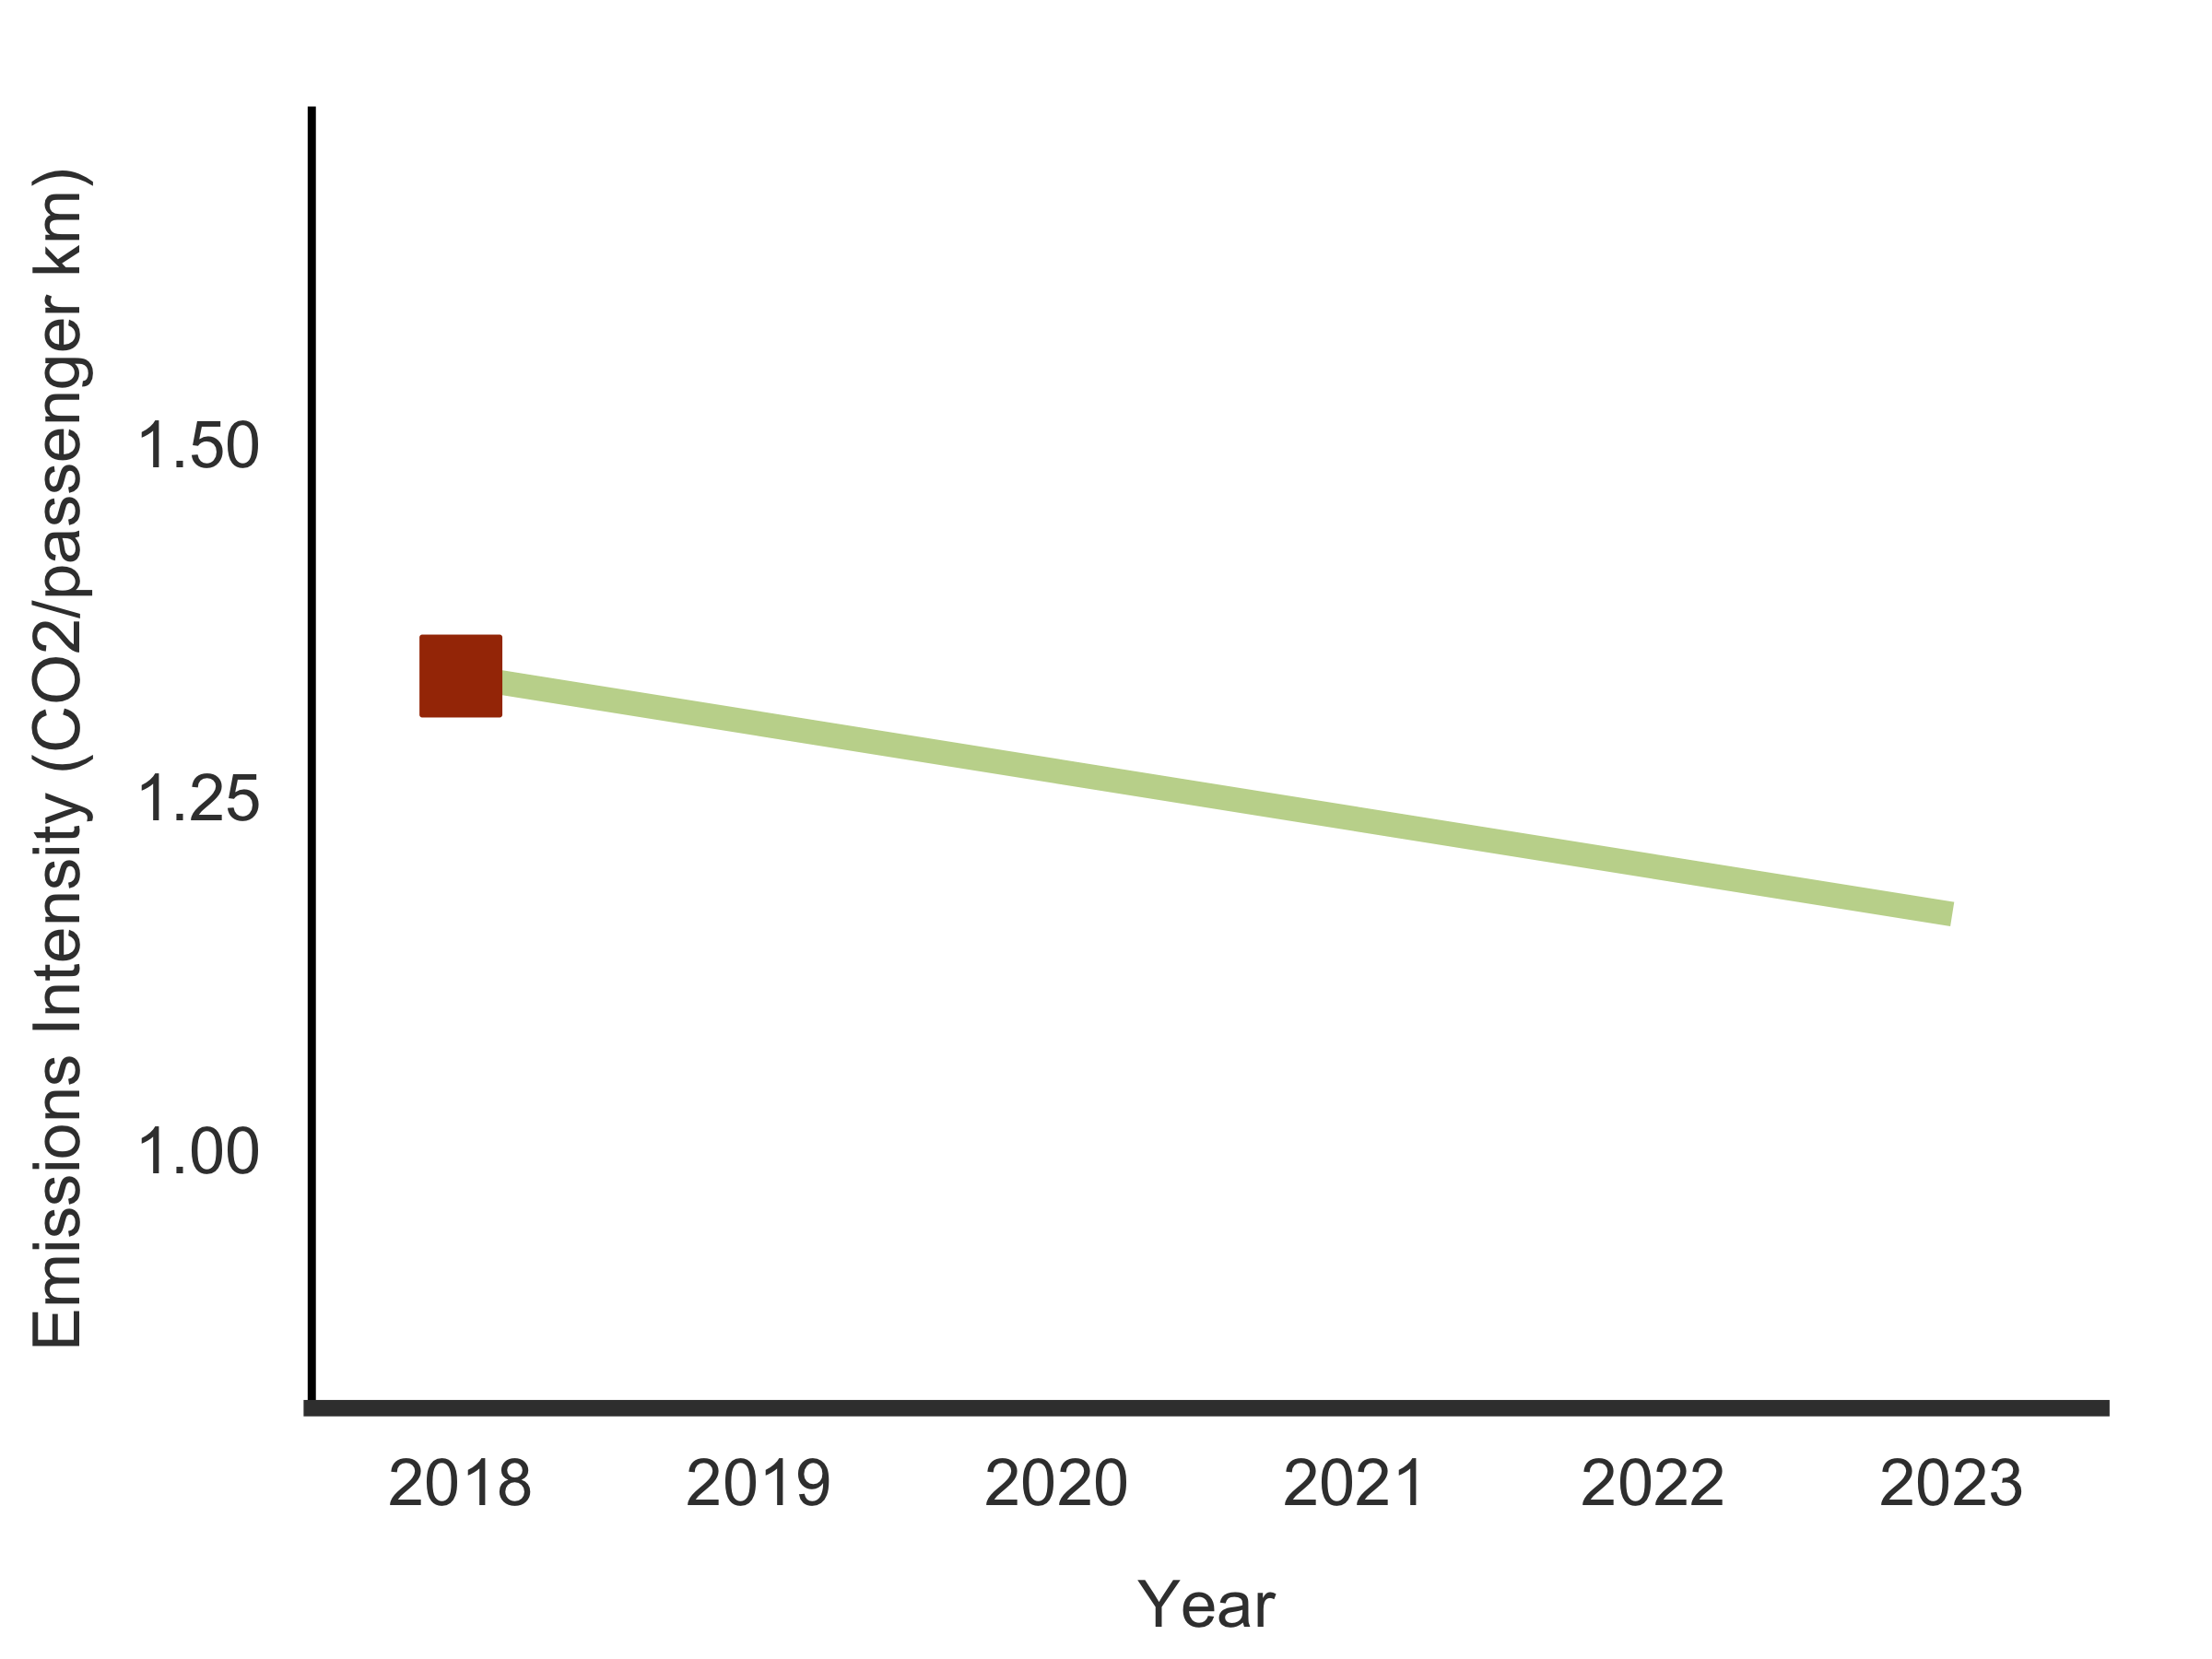
\includegraphics[trim = {0 0cm 0 0},width=1\linewidth]{CAFigures/Fig32}
\end{center}

Wood Mackenzie propose that while shifting away from high-carbon fuels towards low carbon is necessary, within the oil and gas industry, shifting away from particular extraction methods is a transitional alternative. This report does not comment on the emissions by extraction type however data is available on this. Companies need to look beyond resource themes and review the variations in upstream emissions intensity to see how companies can reduce their  CO2 footprints. Even assets of the same theme can have significantly different emissions intensity based upon maturity, location and other unique factors.


\begin{center}
	
	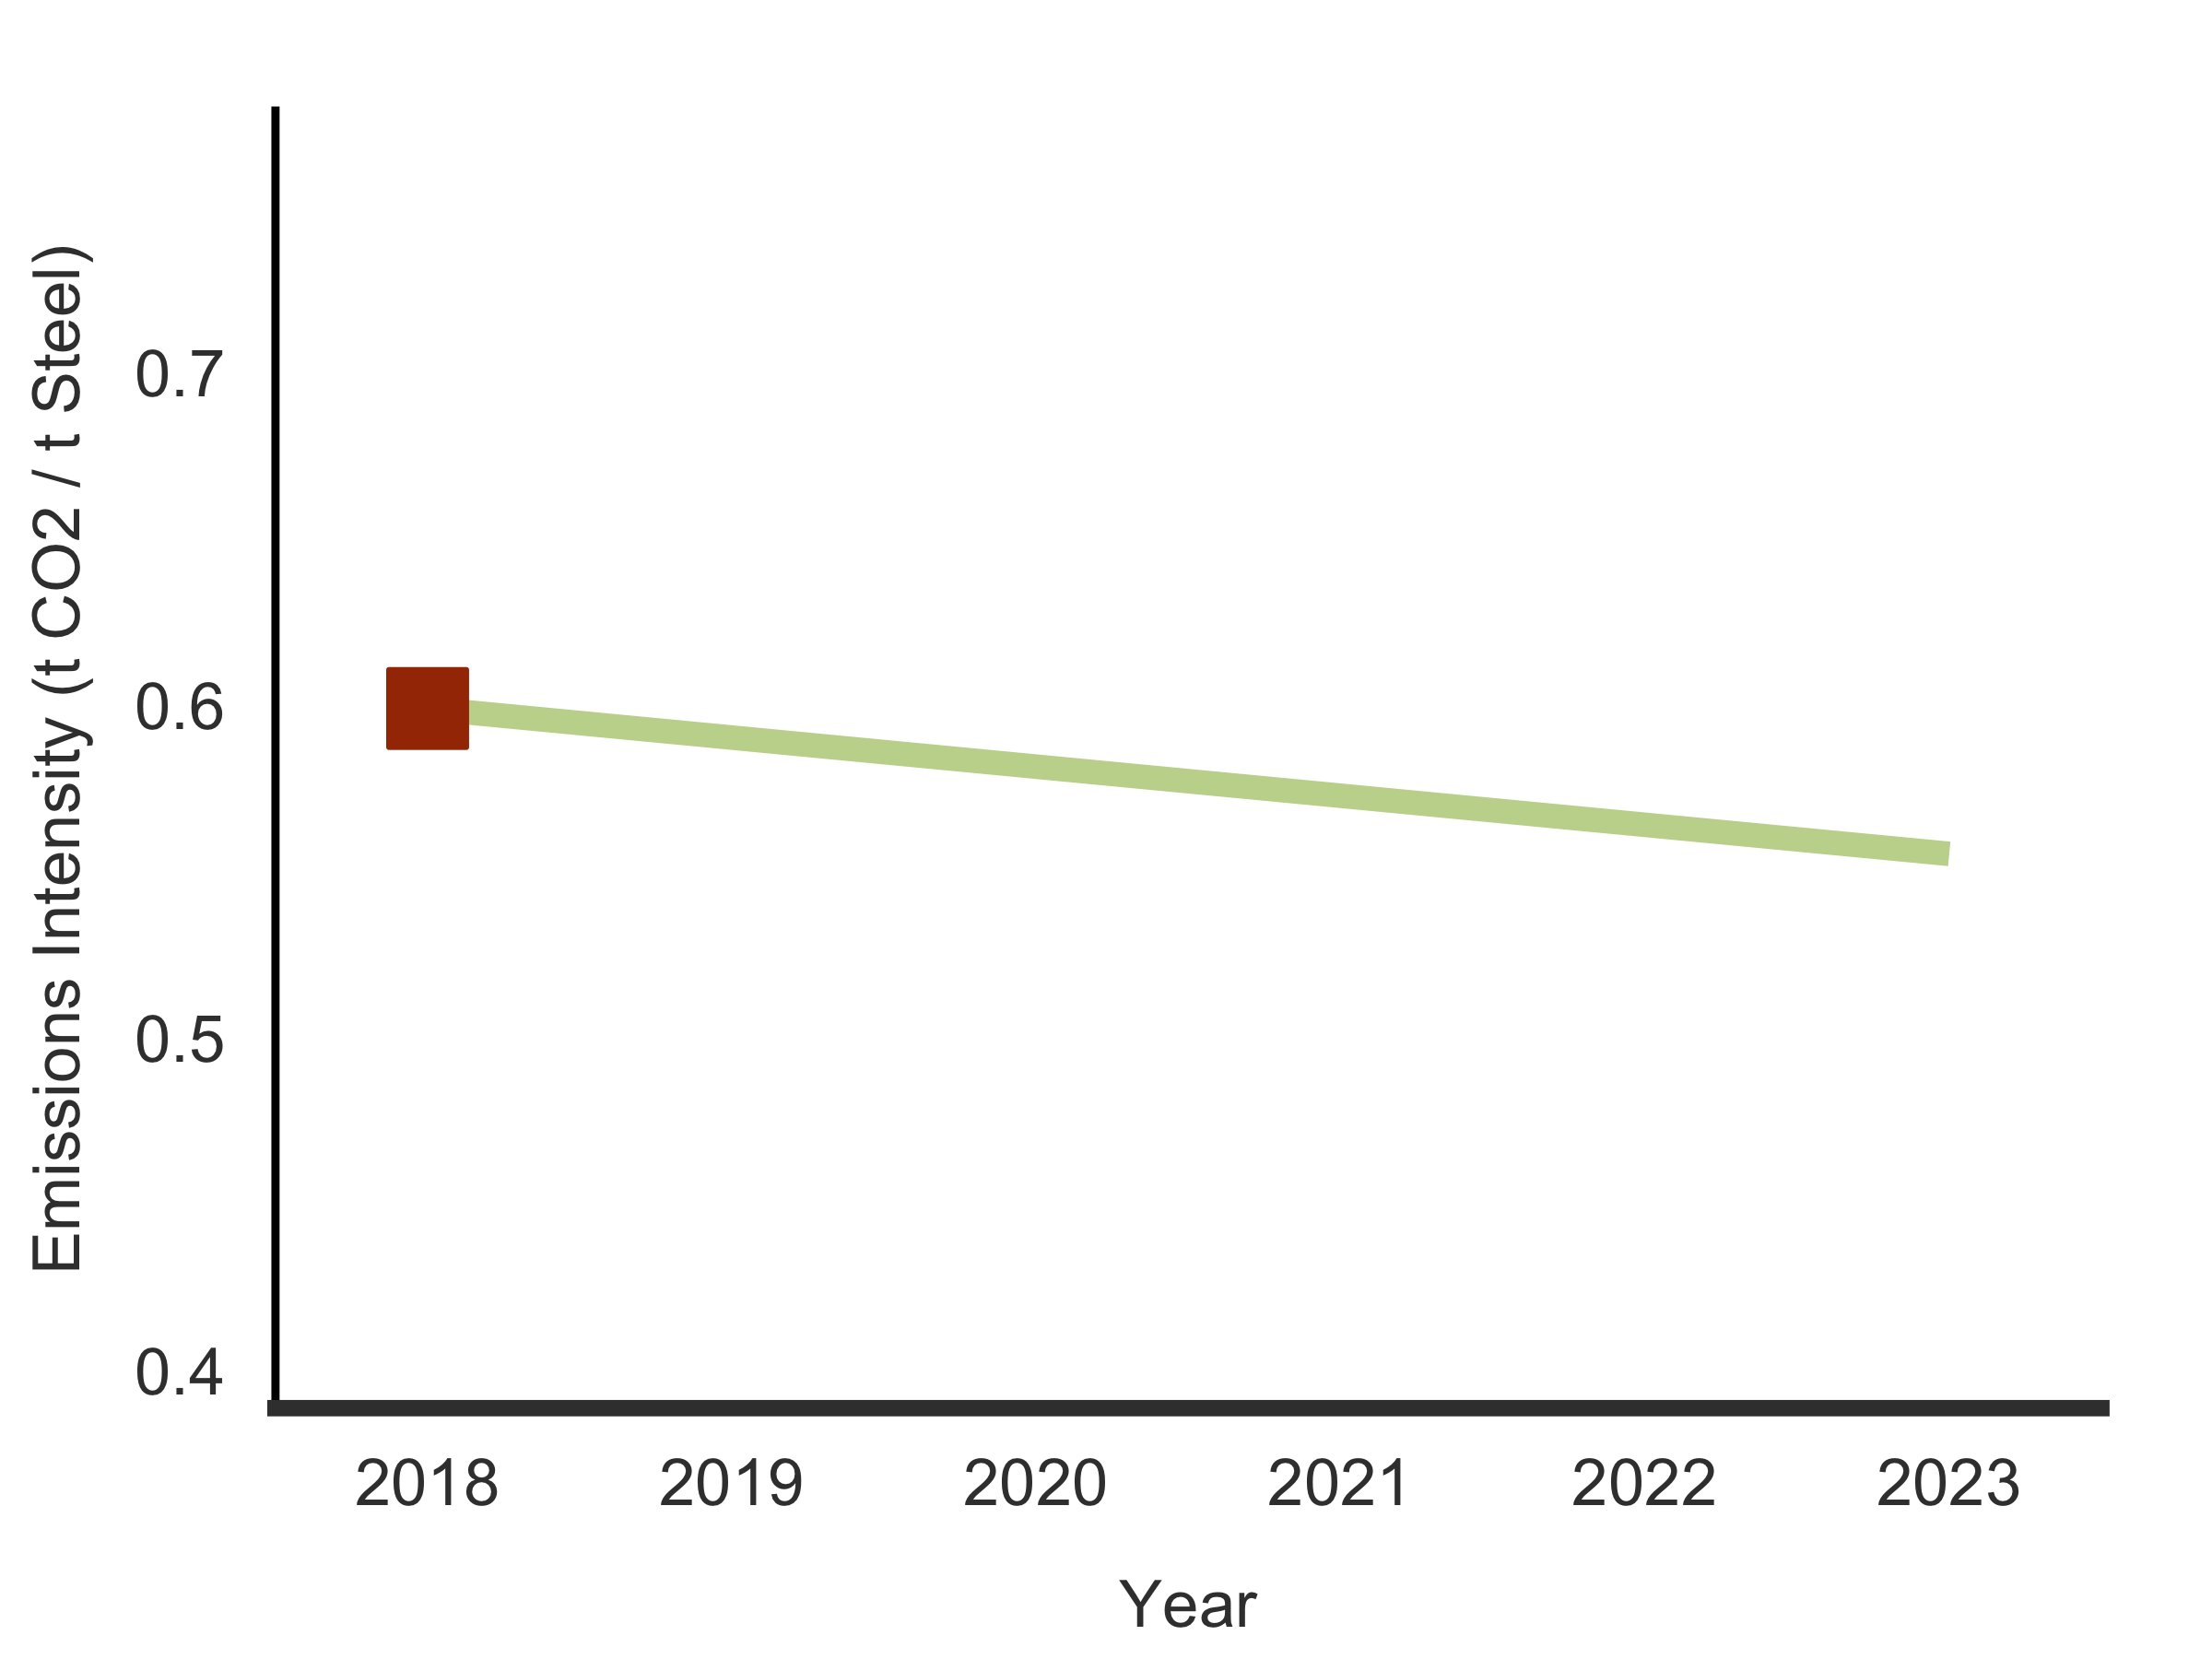
\includegraphics[trim = {0 0cm 0 0},width=1\linewidth]{CAFigures/Fig31}
\end{center}


	\newpage	
\section*{P22} % BACKGROUND
\thispagestyle{empty}
\vspace{17cm}
\SectionHeading{Section 5:}{BACKGROUND}


\newpage	
\section*{P23} %BACKGROUND TO THE MODEL
\PageHeading{BACKGROUND TO THE MODEL}

\textbf{The objective of the assessment framework applied in this scenario analysis is to measure the alignment of financial portfolios with 2°C decarbonisation pathways. The model consists of 3 key elements that are detailed in the following pages.}


 \begin{itemize}
 	
\item {Scenarios, notably 2°C scenarios, that form the basis of the analysis and define the benchmark against which portfolio trends are compared. While in theory a range of scenarios can be applied for the model, in the interest of simplification, this analysis will rely on the scenarios of the International Energy Agency. These provide targets for each technology at a regional level. }

\item{Financial portfolios and associated financial data to allow for the portfolio assessment. Within this report, the analysis will be limited to corporate bonds and listed equity portfolio. Funds within your portfolio have been identified and the underlying financial data extracted from Morningstar and included as part of your portfolio. }

\item{Physical / industry ‘asset level data’ (current and forward looking) is mapped to companies, parents, and securities. This allows the link between financial portfolios  and industry and production data (oil and gas production, automotive production, utilities) to be established. Consequently, this allows a comparison to the 2°C scenarios and a corresponding evaluation of the alignment of the portfolio. }

 \end{itemize}

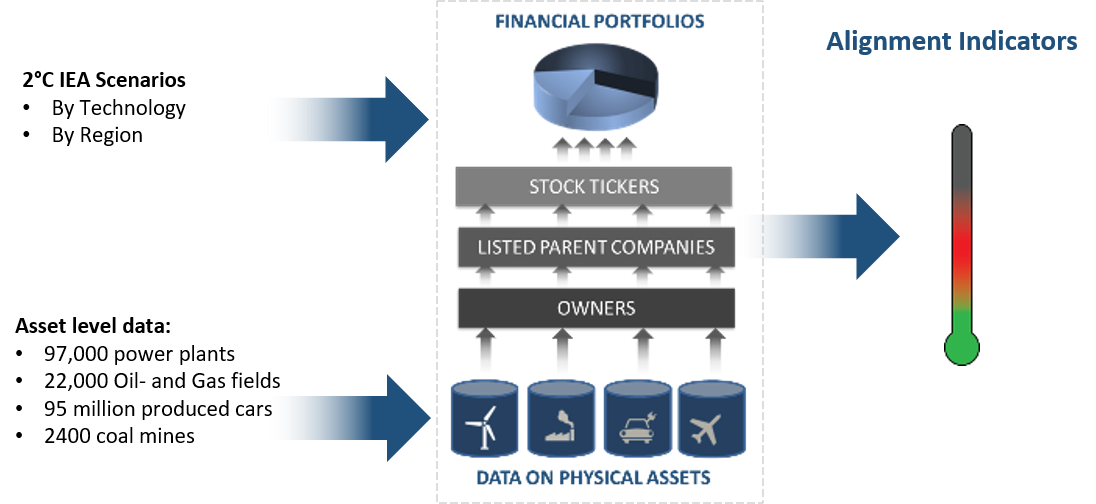
\includegraphics[trim = {0 0cm 0 0},width=1\linewidth]{ReportGraphics/SummaryChart}

\textbf{Allocation Rules}
Based on the financial data, the asset level data is allocated to your portfolio to quantify a representative value of what your portfolio physically owns.  This allocation rules varies between equity and corporate bond portfolios. For equity portfolios, the analysis is based on the ownership percentage of companies and their subsidiaries, with respect to all outstanding shares of the companies. This approach reflects the fact that the shares represent ownership ratios. In the case of bonds, exposure is determined based on the share in the portfolio of the relevant credit instrument. The underlying company exposure is defined by the technology mix (for example, the ratio of renewable to coal power). 

\textbf{Benchmarking}
Using the allocated production or capacity of technologies within your portfolio in as a starting point, an allowance based on the regional scenarios is calculated. This is extrapolated over the next 5 years to create the trajectory and this is compared to your current and future ownership. The variation of your ownership from this benchmark is used as the alignment indicator in the preceding results.  


\newpage	
\section*{P24} %BACKGROUND TO THE MODEL
\PageHeading{BACKGROUND TO THE MODEL}

\textbf{SCENARIOS}

As outlined above, the underlying principle of the model is to compare the portfolio trends with a 2°C scenario. The model for this pilot relies on the International Energy Agency 2°C scenarios (labelled the 450 or 2D Scenario). A common, internationally recognized scenario framework was chosen to ensure comparability across results. The choice of the scenario should not be interpreted however as an endorsement of the underlying assumptions within the model and does not constitute an implicit or explicit assumption around the alignment with long-term climate policy positions. 

The IEA historically has assumed significant amounts of nuclear power and carbon capture and storage in their scenarios. In addition, the international community has accelerated their global target from the 2°C goal to well below 2°C with a target of 1.5°C. It is important to highlight that each investor can and may want to take an individual view on the likely decarbonization scenario that may or may not relate to the scenarios modelled by the International Energy Agency or others.

The model uses the following indicators from the International Energy Agency scenario against which the portfolio is compared:
\begin{itemize}
	\item{Electric capacity by fuel expressed in MW (e.g. renewables, coal, gas, oil, hydropower, nuclear);}
	\item{Oil production expressed in barrels of oil produced / year;}
	\item{Gas production expressed in bcf / year;}
	\item{Coal produced expressed in mtoe / year;}
	\item{GHG emissions pathways in a sample of additional sectors (e.g. aviation, shipping, cement, steel).}
\end{itemize}


\textbf{ASSET LEVEL DATA}

The Asset Level data is sourced from the following data providers: 
\begin{itemize}
	\item{GlobalData (Power plant data, including plants classified as active, announced, financed, partially active, permitting, temporarily shutdown, under construction, under rehabilitation and modernization, and Oil and Gas production data and forecast until 2018-2023, as well as coal mining data); }
	\item{WardsAuto (light passenger duty vehicle, including BAU production forecasts 2018-2023); }
	\item{Bloomberg (financial data);}
	\item{Orbis (database on matching company subsidiary trees);}
	\item{S\&P Cross-Reference Services (database matching securities to parents);}
	\item{Morningstar (database on funds). }
	
\end{itemize}

\textbf{CAVEATS / NOTES ON INTERPRETING THE RESULTS }

The following briefly highlights key caveats to the model and the results:

\begin{itemize}
	\item{The forward-looking data is based on current ‘revealed’ plans from companies and is subject to change. The estimates should thus not be interpreted as final forecasts, but rather the current plans of companies if they don’t change. Another way to interpret the results is the call for action with regard to the required change to align with the 2°C economic trend. Given the 5 year time horizon, there is a high degree of certainty that plans will still change in some way over time. Similarly, the participating financial institutions can of course alter their portfolio exposures over time. The analysis however seeks to be a point in time assessment of future exposures under current conditions.}
	\item{The model takes a diversified ‘market portfolio’ as a basis, focusing on key technologies reflected in the IEA roadmaps. By extension, thematic portfolios invested in breakthrough technologies and / or SRI portfolios with a range of environmental, social, and governmental considerations may not value these elements.}
\end{itemize}

\newpage	
\section*{P24} %INTERPRETATION AND IMPLICATIONS FOR RISK
\PageHeading{INTERPRETATION AND IMPLICATIONS FOR RISK}

 Important in the implementation of different actions based on the 2°C scenario analysis is an understanding of the implications for risk and return of the portfolio. It is important to emphasize here that the results presented in this report are explicitly not a risk analysis. In general, the following findings can be summarized as the interaction between risk, return, and the 2°C scenario analysis. 
 
 \textbf{What is the risk of inaction?}
 Although the analysis focuses on alignment with the Paris Agreement in a way that contributes to the general interest, the issue can also be addressed in terms of the financial risk to the investor if the energy transition is not properly anticipated. 
 
 For investors, the main risk seems to be more pronounced if the 2°C target is not reached. Aviva and the Economist Intelligence Unit analyzed the net impairment loss for financial assets under management at approximately USD60 trillion in a 2°C scenario (Aviva 2015). The TCFD (Task Force on Climate-related Financial Disclosures) initiated by the Financial Stability Committee (FSB) calls these risks ”physical risks”. If the 2°C objective is achieved, these physical risks can be reduced considerably. The cost would be limited to less than USD10 trillion if we remain below 3°C according to the same Aviva / ECIU estimates. 
 
 However, investment portfolios can then be exposed to what the TCFD calls ”transition risks” - the economic and financial risks associated with the transition to a low-carbon economy. These risks are likely to be particularly pronounced for the most CO2-emitting sectors, and thus their investors. Most of these sectors are covered by our analysis in the previous sections. 
 
 Although the 2°C scenario presented in this report is not directly a financial risk assessment, it can help to better understand the exposure to transition risk faced by investors. It makes it possible to understand whether the necessary transition will be gradual (when the production and investment plans are aligned with the 2°C scenario) or is likely to be abrupt (sudden correction linked to the introduction of new technologies or constraints legal proceedings leading to bankruptcies of established companies). All investment strategies are exposed to potential risks. The scenario analysis reveals how each strategy evaluated is an explicit or implicit bet on a 2°C, 4°C or 6°C scenario. Depending on the trajectory that will ultimately prevail, the portfolios will underperform or outperform. From the point of view of the optimization of the risk/return ratio in the long term, it is essential to be aware of the bet made.
 
 From a transition risk perspective, the following three questions are important:
 
 \begin{enumerate}
 	\item{Is my portfolio over-exposed to transition risks by deviating from the 2°C benchmark?}
 	\item{If this is the case, which securities in my portfolio are exposed to these risks?}
 	\item{Should these risks arise, what are possible losses?}
 \end{enumerate}
 
 
 The answer to the first question is provided by the analysis presented in the previous pages. There are different approaches to quantifying exposure:
 
 \begin{itemize}
 	 \item{Based on the method presented in this report, it is possible to isolate the most misaligned sectors and securities with respect to a 2°C trajectory.}
 	
	\item{The rating agency Moody’s developed in 2016 a methodology to classify the different sectors of their corporate bond universe according to the risk of downgrade due to environmental risk.}
 \end{itemize}
 
 
 \textbf{Asset Pricing and Risk} 
 A final question to be considered is: what is the potential value at risk within the climate relevant sectors if a 2° C scenario materializes? This requires additional financial analysis. In particular, assumptions must be made as to how the market has already (or not) integrated these risks into the current price of financial assets. There are several research papers on the subject, published by financial analysts, NGOs and consultants, covering equities and credit (2ii 2018). 
 
 In all this, it is important to emphasize that asset prices - based on market participants’ assumptions about changes in the yield-risk profile of securities - do not necessarily reflect the economic risks faced by a company. Thus, the price of assets , and the risk that their valuation will decrease, does not automatically reflect the underlying risks to which the companies are exposed. On the other hand, it should be noted that the return potential is optimized when the allocation of capital is as efficient as possible. If the capital is not allocated efficiently, the absolute benefit is also reduced. Signals issued by the financial markets in the form of portfolio reallocation choices or via shareholder engagement can thus help optimize the allocation of capital in the real economy, and help maximize long-term returns.
 
\newpage	
\section*{P25} %NOTES AND DISCLAIMER
\PageHeading{NOTES AND DISCLAIMER}

The data and scenario sources for this analysis are shown below. 

\textbf{Published Research}

The methodology behind this scenario analysis, the accounting rules applied, and further information to the scenarios and data can be found in the following published research papers. 

Accounting Principles: http://www.mdpi.com/2071-1050/10/2/328 
Scenario Work: http://et-risk.eu/toolbox/scenarios/ 
Asset Level Data Analysis: http://2degrees-investing.org/IMG/pdf/assetdata\_v0.pdf

\textbf{Sources for the data and scenario analysis}

Automobile data are from July 2018 and is provided by WardsAuto / AutoForecastSolutions. Power data is from July 2018 and is provided by GlobalData. Oil, gas and coal production data is from July 2018 and is provided by GlobalData. When linking asset data with companies, the data is used by the data providers mentioned above and, where possible, enriched with company data from Bloomberg. All financial data, as well as identification numbers for linking company data with financial instruments, come from Bloomberg. The decarbonization pathways for other sectors comes from the Science-Based Targets Initiative, which bases its methodology on the IEA scenarios. The scenarios for the energy and power sector come from the IEA’s World Energy Outlook 2016. Because this report does not include scenario information for the automotive sector, the related data is taken from the sister report of the World Energy Outlook, the Energy Technology Perspective report. Benchmarks for the electricity sector are determined regionally and applied in relation to the regional exposure data and then aggregated, weighted according to the regional exposure of the portfolio. All other results are global.

\textbf{Sources}

IPCC (2018) https://www.ipcc.ch/report/ar5/
FSB (2018) https://www.fsb-tcfd.org/publications/final-recommendations-report/
Aviva / ECIU (2015) https://www.aviva.com/media/thought-leadership/climate-change-value-risk-investment-and-avivas-strategicresponse/
FSB (2018) https://www.fsb-tcfd.org/publications/final-recommendations-report/
WoodMackenzie (2018) https://www.woodmac.com/news/editorial/carbon-intensity-not-all-assets-are-created-equal/ 

\textbf{Disclaimer}

The 2° Investing Initiative’s research is provided free of charge and 2°ii does not seek any direct or indirect financial compensation for its research. 2°ii is not an investment adviser and makes no representation regarding the advisability of investing in any particular company or investment fund or other vehicle. A decision to invest in any such investment fund or other entity should not be made in reliance on any of the statements set forth on this website and the analysis results. The information and analysis contained in this research report does not constitute an offer to sell securities or the solicitation of an offer to buy, or recommendation for investment, in any securities within the United States or any other jurisdiction. The information is not intended as financial advice. The research report and website results provide general information only. The information and opinions constitute a judgment as at the date indicated and are subject to change without notice. No representation or warranty, express or implied, is made by 2°ii as to their accuracy, completeness or correctness. 2°ii does not warrant that the information is up to date, nor does it take liability for errors in third-party sourced data.


\end{document}



